\documentclass[10pt,compress]{beamer}
%\documentclass[fleqn,xcolor=dvipsnames]{beamer}
\usetheme{Madrid}
%\usetheme{Boadilla}
%\usetheme{default}
%\usetheme{Warsaw}
%\usetheme{CambridgeUS}
%\usetheme{Sybila}
%\usetheme[hideothersubsections]{Berkeley}
%\usetheme[hideothersubsections]{PaloAlto}
%%\usetheme[hideothersubsections]{Goettingen}
%\usetheme{CambridgeUS}
%\usetheme{Bergen} % This template has nagivation on the left
%\usetheme{Frankfurt} % Similar to the default with an extra region at the top.

% Uncomment the following line if you want page numbers and using Warsaw theme%
%\setbeamertemplate{footline}[page number]

\definecolor{aggiemaroon}{RGB}{80,0,0} % Official RGB code for aggie maroon
\usecolortheme[named=aggiemaroon]{structure}
\useoutertheme{shadow}
\useinnertheme{rounded}
\setbeamertemplate{navigation symbols}{}
\setbeamerfont{structure}{family=\rmfamily,series=\bfseries}
\usefonttheme[stillsansseriftext]{serif}

\usepackage{amsmath}
\usepackage{caption}
\usepackage{graphicx,comment}
\usepackage[english]{babel}
\usepackage{rotating}
\usepackage{multicol}
\usepackage{enumerate}
\usepackage{tikz}
\usepackage{bm}
\usepackage{listings}
\usepackage{minted}
\usepackage{hyperref} %always the last to avoid problems


\usebackgroundtemplate{
\tikz\node[opacity=0.035, rotate = 0] {
\includegraphics[scale=0.5]{UPM-logo.png}};}
%{
\includegraphics[height=1in,width=1in]{TAM-Logo.png}};}


\title[Universidad Politecnica de Madrid]{Embedded System Design with Raspberry-pi}

\author [M. Ruiz]{Mariano Ruiz}

\date[01/15/2025]{January 15, 2025}

\institute[UPM] % (optional, but mostly needed)
{\emph{Professor}, ETSI Sistemas de Telecomunicación Copiado de Bootlin \\
 
\includegraphics[scale=0.60]{UPM-logo.png} \\ [0.0 cm]
 }



\AtBeginSection[]
{
  \begin{frame}<beamer>
   % \frametitle{Section \thesection} %this add the section number only
   \frametitle{\insertsectionhead}
    \tableofcontents[currentsection, hideallsubsections]
  \end{frame}
}
%\newcommand{\codelink}[1]{\texttt{#1}}

\newcommand{\codecolor}{\usebeamercolor[fg]{code}}
\newcommand{\code}[1]{{\codecolor \path{#1}}}
\newcommand{\codelink}[1]{{\usebeamercolor[fg]{darkblue} \path{#1}}}
\newcommand{\codewithhash}[1]{{\codecolor \tt{#1}}}
%\newcommand{\code}[1] {\path{#1}}

\newcommand\projdir[2]{\href{https://elixir.bootlin.com/#1/latest/source/#2/}{\codelink{#2/}}}
\newcommand\projfile[2]{\href{https://elixir.bootlin.com/#1/latest/source/#2}{\codelink{#2}}}
\newcommand\kconfig[1]{\href{https://elixir.bootlin.com/linux/latest/K/ident/#1}{\codelink{#1}}}
\newcommand\kconfigval[2]{\href{https://elixir.bootlin.com/linux/latest/K/ident/#1}{\codelink{#1=#2}}}
\newcommand\kdir[1]{\projdir{linux}{#1}}
\newcommand\kfile[1]{\projfile{linux}{#1}}
\newcommand\kfileversion[2]{\href{https://elixir.bootlin.com/linux/v#2/source/#1}{\codelink{#1}}}
\newcommand\kstruct[1]{\href{https://elixir.bootlin.com/linux/latest/ident/#1}{\codelink{struct #1}}}
\newcommand\kdochtml[1]{\href{https://www.kernel.org/doc/html/latest/#1.html}{\codelink{#1}}}
\newcommand\kdochtmldir[1]{\href{https://www.kernel.org/doc/html/latest/#1/}{\codelink{#1/}}}

\begin{document}

\begin{frame}
\titlepage
\end{frame}

%\begin{frame}
%\frametitle{Overview} 
%\tableofcontents
%\end{frame}

\newcommand{\training}{linux-kernel}
\graphicspath{{trainingmaterials/}}
\section{Introduction to Embedded Linux}

\begin{frame}
  \frametitle{Birth of Free Software}
  \begin{columns}
    \column{0.75\textwidth}
      \begin{itemize}
      \item 1983, Richard Stallman, {\bf GNU project} and the {\bf free
          software} concept.  Beginning of the development of {\em gcc},
        {\em gdb}, {\em glibc} and other important tools
      \item 1991, Linus Torvalds, {\bf Linux kernel project}, a UNIX-like
        operating system kernel. Together with GNU software and many other
        open-source components: a completely free operating system,
        GNU/Linux
      \item ~1995, Linux is more and more popular on server systems
      \item ~2000, Linux is more and more popular on {\bf embedded
          systems}
      \item ~2008, Linux is more and more popular on mobile devices and phones
      \item ~2012, Linux is available on cheap, extensible hardware:
            Raspberry Pi, BeagleBone Black
      \end{itemize}
    \column{0.25\textwidth}
      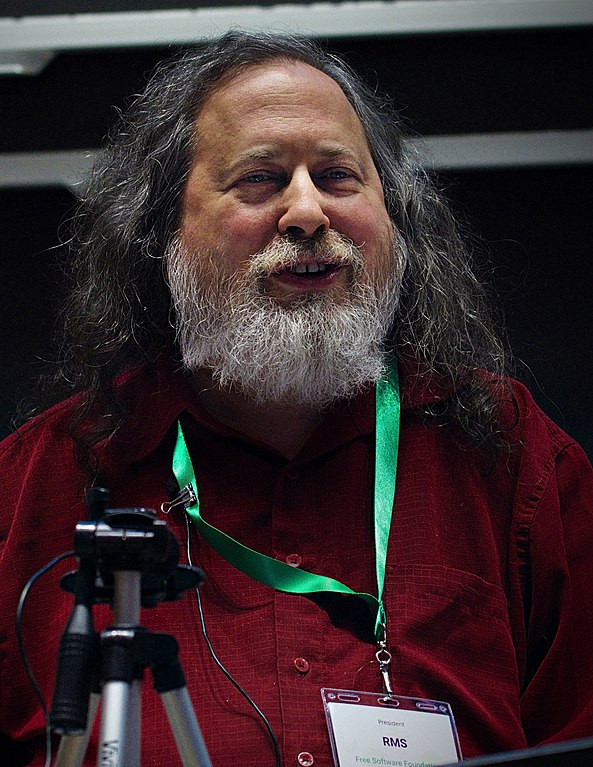
\includegraphics[width=\textwidth]{slides/sysdev-intro/richard-stallman.jpg}
      \scriptsize
      Richard Stallman in 2019\\
      \tiny \url{https://commons.wikimedia.org/wiki/File:Richard_Stallman_at_LibrePlanet_2019.jpg}
    \end{columns}

\end{frame}

\begin{frame}
  \frametitle{Free software?}
  \begin{itemize}
  \item A program is considered {\bf free} when its license offers to
    all its users the following {\bf four} freedoms
    \begin{itemize}
    \item Freedom to run the software for any purpose
    \item Freedom to study the software and to change it
    \item Freedom to redistribute copies
    \item Freedom to distribute copies of modified versions
    \end{itemize}
  \item These freedoms are granted for both commercial and
    non-commercial use
  \item They imply the availability of source code, software can be
    modified and distributed to customers
  \item {\bf Good match for embedded systems!}
  \end{itemize}
\end{frame}

\begin{frame}{What is embedded Linux?}
  \huge
  \begin{center}
    Embedded Linux is the usage of the {\bf Linux kernel} and various
    {\bf open-source} components in embedded systems
  \end{center}
\end{frame}

\begin{frame}
  \frametitle{Advantages of Linux and Open-Source in embedded systems}
  \footnotesize
  \begin{columns}
  \column{0.5\textwidth}
     \begin{itemize}
     \item {\bf Ability to reuse components}\\
           Many features, protocols and hardware are supported.
           Allows to focus on the added value of your product.
     \item {\bf Low cost}\\
           No per-unit royalties. Development tools free
	   too. But of course deploying Linux costs time and effort.
     \item {\bf Full control}\\
           You decide when to update components in your
	   system. No vendor lock-in. This secures your investment.
     \item {\bf Easy testing of new features}\\
           No need to negotiate with third-party vendors. Just explore
	   new solutions released by the community.
     \end{itemize}
  \column{0.5\textwidth}
     \begin{itemize}
     \item {\bf Quality}\\
           Your system is built on high-quality foundations
           (kernel, compiler, C-library, base utilities...). Many
           Open-Source applications have good quality too.
     \item {\bf Security}\\
           You can trace the sources of all system components
           and perform independent vulnerability assessments.
     \item {\bf Community support}\\
           Can get very good support from the
	   community if you approach it with a constructive attitude.
     \item {\bf Participation in community work}\\
	   Possibility to collaborate with peers and get opportunities
           beyond corporate barriers.
     \end{itemize}
  \end{columns}
\end{frame}

\subsection[Systems running Linux]{A few examples of embedded systems
  running Linux}

\begin{frame}
  \frametitle{Wireless routers}
  \begin{center}
    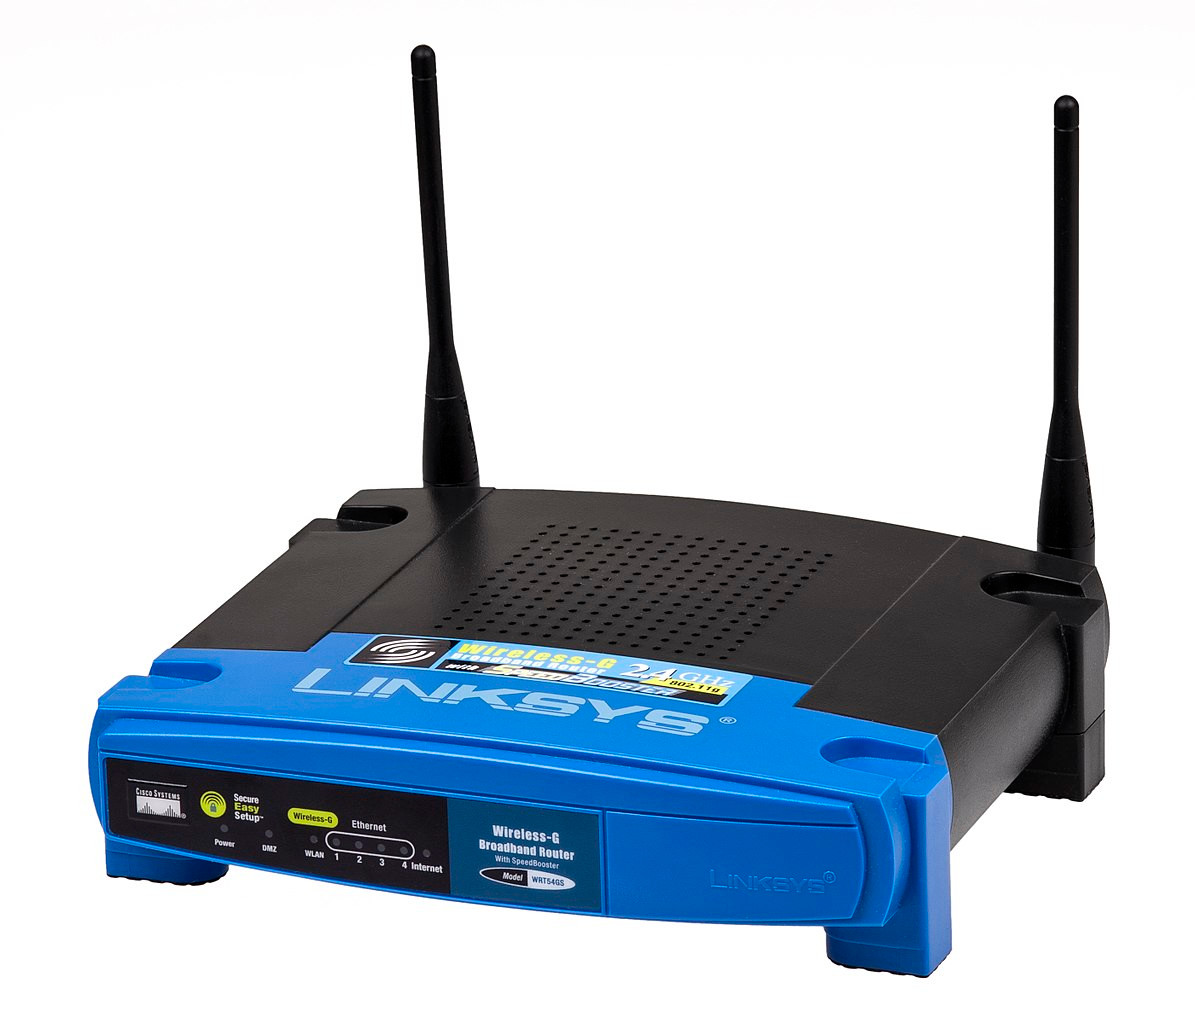
\includegraphics[height=0.8\textheight]{slides/sysdev-intro/linksys-wireless-router.jpg}
  \end{center}
  \tiny
  Image credits: Evan Amos (\url{https://bit.ly/2JzDIkv})
\end{frame}

\begin{frame}
\frametitle{Video systems}
  \begin{center}
    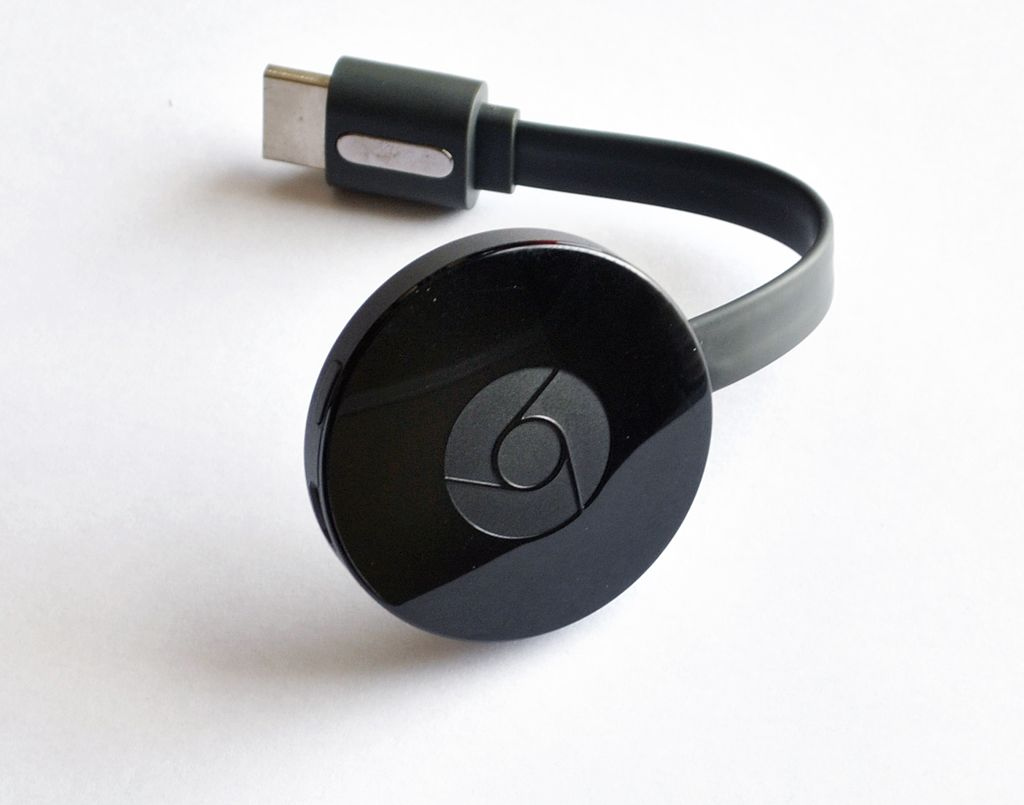
\includegraphics[height=0.8\textheight]{slides/sysdev-intro/chromecast-2015.jpg}
  \end{center}
  \tiny Image credits: \url{https://bit.ly/2HbwyVq}
\end{frame}

\begin{frame}
\frametitle{Bike computers}
  \begin{center}
    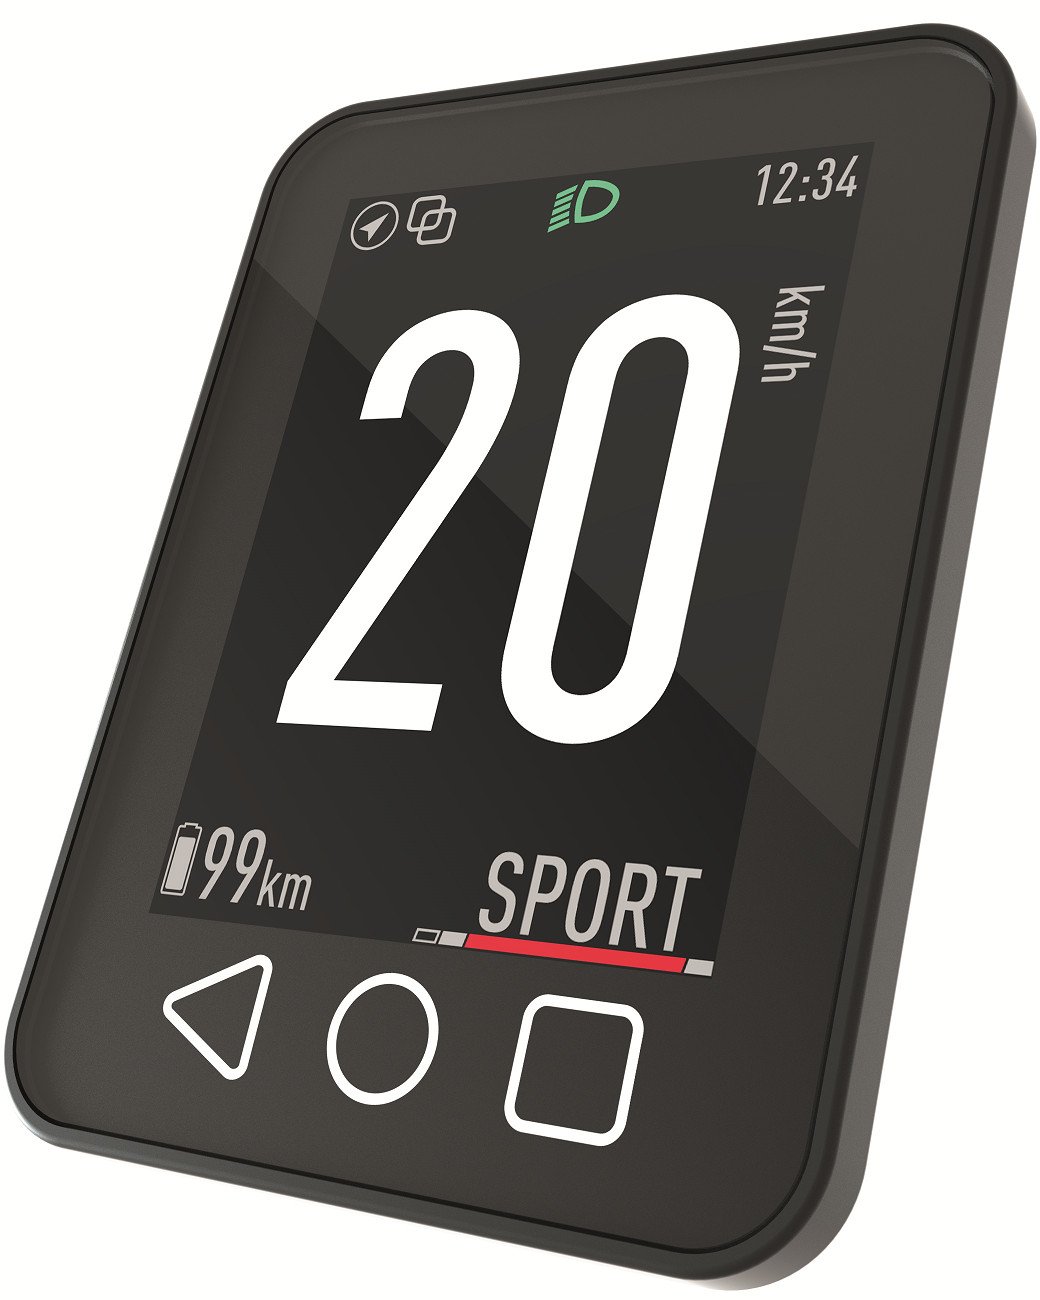
\includegraphics[height=0.8\textheight]{slides/sysdev-intro/bike-computer.jpg}
  \end{center}
  \tiny
  Product from BLOKS (\url{http://bloks.de}).
  Permission to use this picture only in this document, in updates and
  in translations.
\end{frame}

\begin{frame}
\frametitle{Robots}
  \begin{center}
    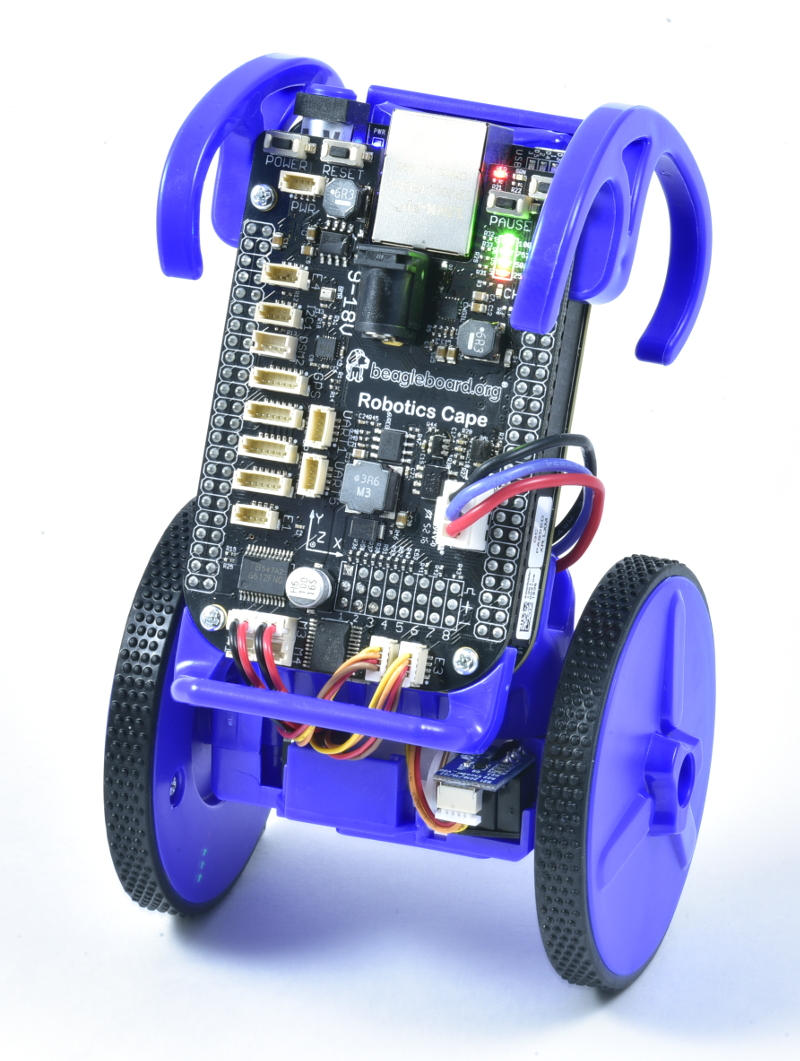
\includegraphics[height=0.75\textheight]{slides/sysdev-intro/beagle-robot.jpg}
  \end{center}
  eduMIP robot (\url{https://www.ucsdrobotics.org/edumip})
\end{frame}

\begin{frame}
\frametitle{In space}
  \begin{columns}
  \column{0.5\textwidth}
  \scriptsize
  SpaceX Starlink satellites\\
  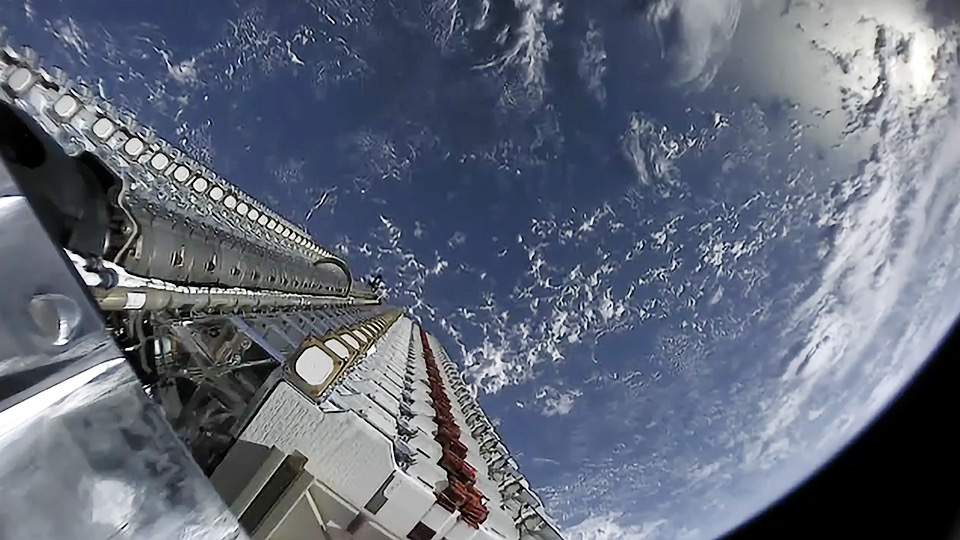
\includegraphics[height=0.3\textheight]{slides/sysdev-intro/starlink.jpg}\\
  SpaceX Falcon 9 and Falcon Heavy rockets\\
  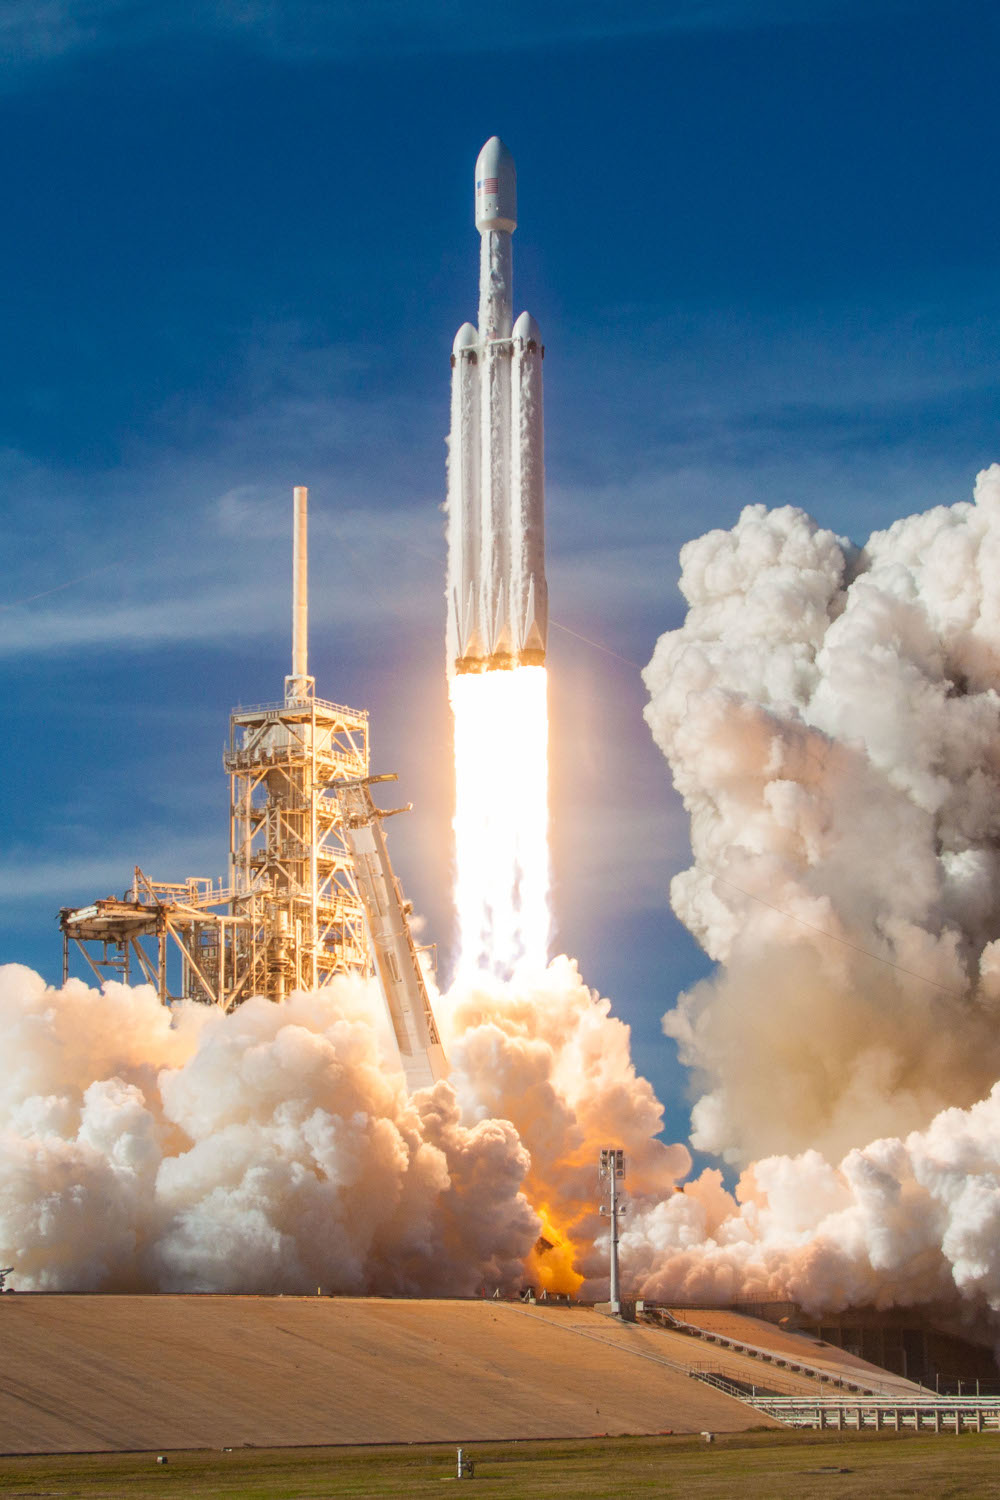
\includegraphics[height=0.3\textheight]{slides/sysdev-intro/falcon-heavy.jpg}\\
  \vspace{0.3cm}
  \tiny Image credits: Wikipedia
  \column{0.5\textwidth}
  \scriptsize
  Mars Ingenuity Helicopter\\
  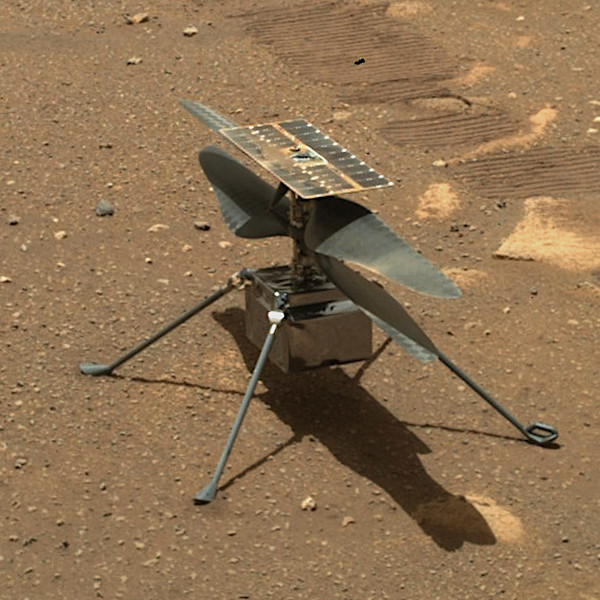
\includegraphics[height=0.3\textheight]{slides/sysdev-intro/mars-helicopter.jpg}\\
  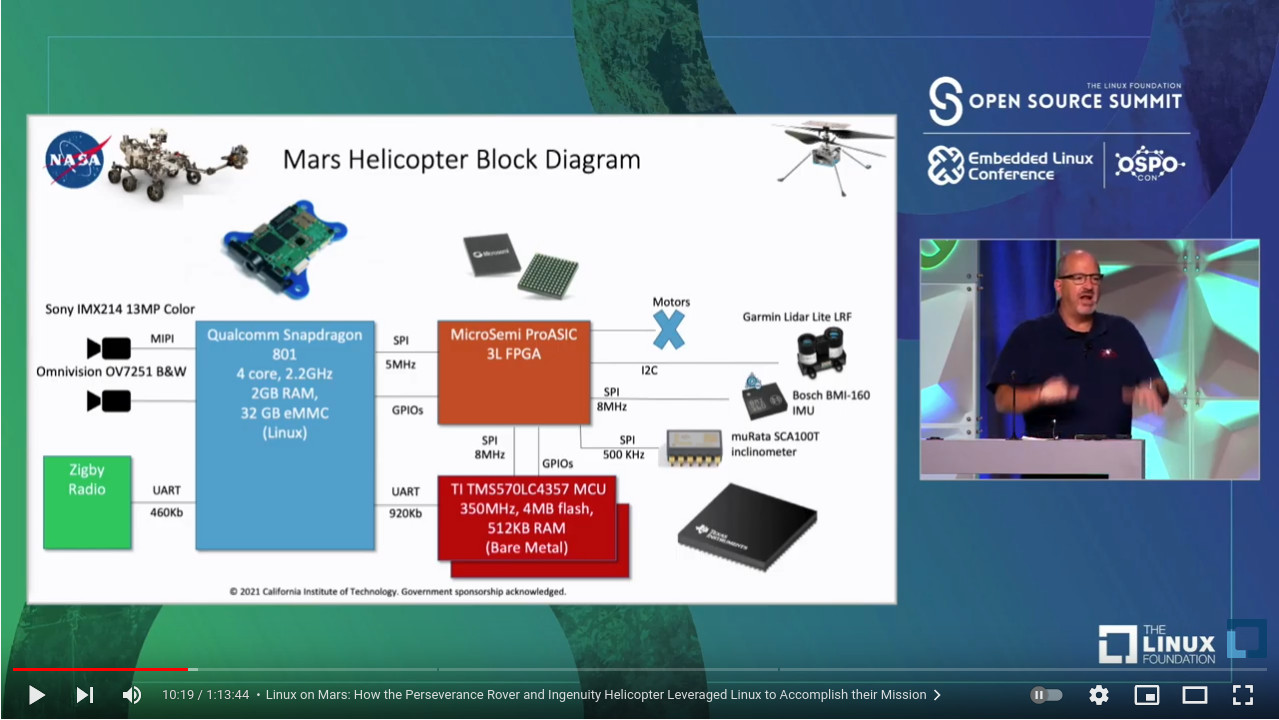
\includegraphics[height=0.3\textheight]{slides/sysdev-intro/mars-helicopter-video.jpg}\\
  \vspace{0.5cm}
  \tiny
  See the {\em Linux on Mars: How the Perseverance Rover and Ingenuity Helicopter Leveraged
  Linux to Accomplish their Mission} presentation from Tim Canham (JPL, NASA):
  \url{https://youtu.be/0_GfMcBmbCg?t=111}
  \end{columns}
\end{frame}

\subsection{Embedded hardware for Linux systems}

\begin{frame}
  \frametitle{Processor and architecture (1)}
  The Linux kernel and most other architecture-dependent
  components support a wide range of 32 and 64 bit architectures
  \begin{itemize}
  \item x86 and x86-64, as found on PC platforms, but also embedded systems
    (multimedia, industrial)
  \item ARM, with hundreds of different {\em System on Chip}s\\
        ({\em SoC}: CPU + on-chip devices, for all sorts of products)
  \item RISC-V, the rising architecture with a free instruction set\\
        (from high-end cloud computing to the smallest embedded systems)
  \item PowerPC (mainly real-time, industrial applications)
  \item MIPS (mainly networking applications)
  \item Microblaze (Xilinx), Nios II (Altera): soft cores on FPGAs
  \item Others: ARC, m68k, Xtensa, SuperH...
  \end{itemize}
\end{frame}

\begin{frame}
  \frametitle{Processor and architecture (2)}
  \begin{itemize}
  \item Both MMU and no-MMU architectures are supported, even though
    no-MMU architectures have a few limitations.
  \item Linux does not support small microcontrollers (8 or 16 bit)
  \item Besides the toolchain, the bootloader and the kernel, all
    other components are generally {\bf architecture-independent}
  \end{itemize}
\end{frame}

\begin{frame}
  \frametitle{RAM and storage}
  \begin{itemize}
  \item {\bf RAM}: a very basic Linux system can work within 8 MB of
    RAM, but a more realistic system will usually require at least 32
    MB of RAM. Depends on the type and size of applications.
  \item {\bf Storage}: a very basic Linux system can work within 4 MB
    of storage, but usually more is needed.
    \begin{itemize}
    \item {\bf Block storage}: SD/MMC/eMMC, USB mass storage, SATA, etc,
    \item {\bf Raw flash storage} is supported too, both NAND and NOR flash, with
      specific filesystems
    \end{itemize}
  \item Not necessarily interesting to be too restrictive on the
    amount of RAM/storage: having flexibility at this level allows to
    increase performance and re-use as many existing components as possible.
  \end{itemize}
\end{frame}

\begin{frame}
  \frametitle{Communication}
  \begin{itemize}
  \item The Linux kernel has support for many common communication
    buses
    \begin{itemize}
    \item I2C
    \item SPI
    \item 1-wire
    \item SDIO
    \item PCI
    \item USB
    \item CAN (mainly used in automotive)
    \end{itemize}
  \item And also extensive networking support
    \begin{itemize}
    \item Ethernet, Wifi, Bluetooth, CAN, etc.
    \item IPv4, IPv6, TCP, UDP, SCTP, DCCP, etc.
    \item Firewalling, advanced routing, multicast
    \end{itemize}
  \end{itemize}
\end{frame}

\begin{frame}
  \frametitle{Types of hardware platforms (1)}
  \begin{columns}
  \column{0.75\textwidth}
  \begin{itemize}
  \item {\bf Evaluation platforms} from the SoC vendor. Usually
    expensive, but many peripherals are built-in. Generally unsuitable
    for real products, but best for product development.
  \item {\bf System on Module} (SoM) or {\bf Component on Module}, a small
    board with only CPU/RAM/flash and a few other core components, with
    connectors to access all other peripherals. Can be used to build end
    products for small to medium quantities.
  \end{itemize}
  \column{0.25\textwidth}
    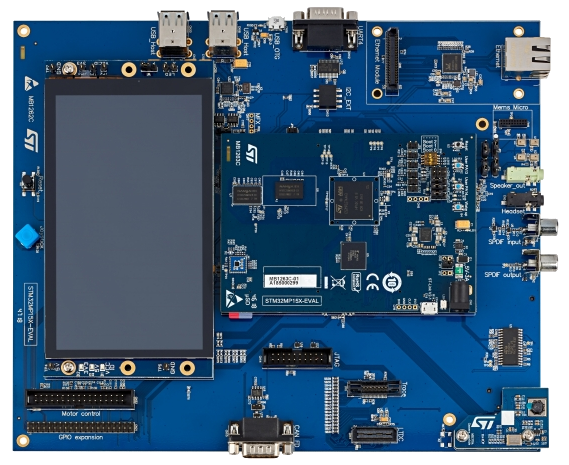
\includegraphics[width=\textwidth]{slides/sysdev-intro/stm32mp157c-ev1.png}
    \scriptsize
    STM32MP157C-EV1 evaluation board\\
    \tiny
    \href{https://www.mouser.fr/ProductDetail/STMicroelectronics/STM32MP157C-EV1?qs=9r4v7xj2LnmHBJ35TLmsRg\%3D\%3D}{Image credits}
    \vspace{0.5cm}
    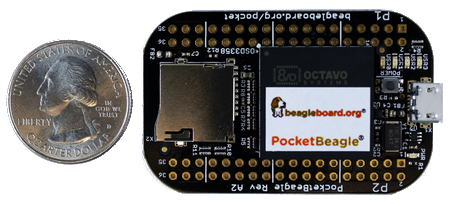
\includegraphics[width=\textwidth]{slides/sysdev-intro/pocketbeagle.png}
    \scriptsize
    PocketBeagle\\
    \tiny
    Image credits (Beagleboard.org):\\
    \url{https://beagleboard.org/pocket}
  \end{columns}
\end{frame}

\begin{frame}
  \frametitle{Types of hardware platforms (2)}
  \begin{columns}
  \column{0.75\textwidth}
  \begin{itemize}
  \item {\bf Community development platforms}, to make a
    particular SoC popular and easily available. These are
    ready-to-use and low cost, but usually have fewer peripherals than
    evaluation platforms. To some extent, can also be used for real
    products.
  \item {\bf Custom platform}. Schematics for evaluation boards or
    development platforms are more and more commonly freely available,
    making it easier to develop custom platforms.
  \end{itemize}
  \column{0.25\textwidth}
    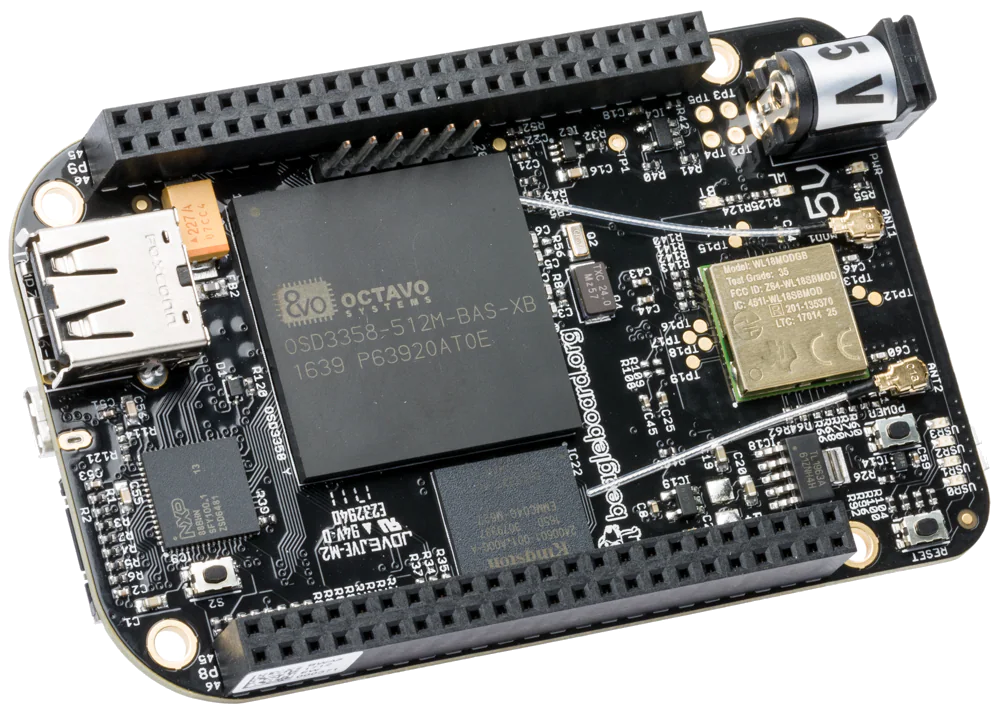
\includegraphics[height=0.3\textheight]{/slides/beagleboneblack-board/beagleboneblack.png}
    \scriptsize
    Beaglebone Black Wireless board\\
    \vspace{0.5cm}
    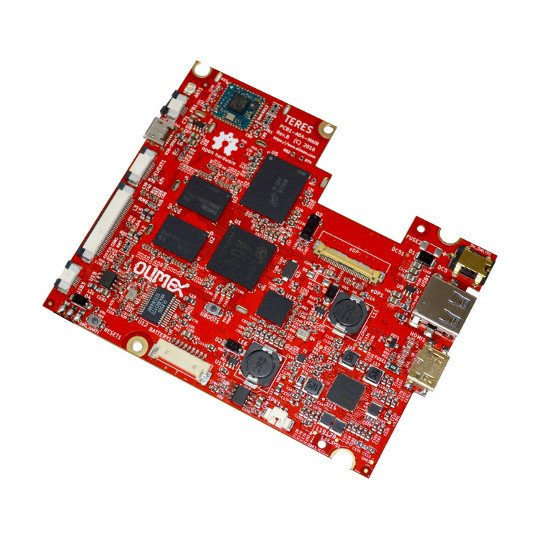
\includegraphics[height=0.3\textheight]{slides/sysdev-intro/teres-pcb1-a64.jpg}
    \scriptsize
    Olimex Open hardware ARM laptop main board\\
    \tiny
    Image credits (Olimex):\\
    \url{https://www.olimex.com/Products/DIY-Laptop/}
  \end{columns}
\end{frame}

\begin{frame}
  \frametitle{Criteria for choosing the hardware}
  \begin{itemize}
  \item Most SoCs are delivered with support for the Linux kernel
    and for an open-source bootloader.
  \item Having support for your SoC in the official versions of the projects
    (kernel, bootloader) is a lot better: quality is better, new
    versions are available, and Long Term Support releases are
    available.
  \item Some SoC vendors and/or board vendors do not contribute their
    changes back to the mainline Linux kernel. Ask them to do so, or
    use another product if you can. A good measurement is to see the
    delta between their kernel and the official one.
  \item {\bf Between properly supported hardware in the official Linux
    kernel and poorly-supported hardware, there will be huge
    differences in development time and cost.}
  \end{itemize}
\end{frame}

\subsection{Embedded Linux system architecture}

\begin{frame}
  \frametitle{Host and target}
  \begin{center}
    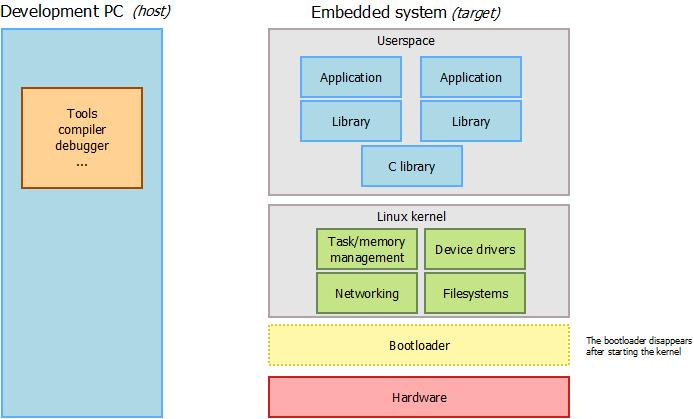
\includegraphics[height=0.8\textheight]{slides/sysdev-intro/host-and-target.jpg}
  \end{center}
\end{frame}

\begin{frame}
  \frametitle{Software components}
  \begin{itemize}
  \item Cross-compilation toolchain
    \begin{itemize}
    \item Compiler that runs on the development machine, but generates
      code for the target
    \end{itemize}
  \item Bootloader
    \begin{itemize}
    \item Started by the hardware, responsible for basic
      initialization, loading and executing the kernel
    \end{itemize}
  \item Linux Kernel
    \begin{itemize}
    \item Contains the process and memory management, network stack,
      device drivers and provides services to user space applications
    \end{itemize}
  \item C library
    \begin{itemize}
    \item Of course, a library of C functions
    \item Also the interface between the kernel and the user space
      applications
    \end{itemize}
  \item Libraries and applications
    \begin{itemize}
    \item Third-party or in-house
    \end{itemize}
  \end{itemize}
\end{frame}

\begin{frame}
  \frametitle{Embedded Linux work}

  Several distinct tasks are needed when deploying embedded Linux in a
  product:

  \begin{itemize}
  \item {\bf Board Support Package development}
    \begin{itemize}
    \item A BSP contains a bootloader and kernel with the suitable
      device drivers for the targeted hardware
    \item Purpose of our \href{https://bootlin.com/training/kernel}
      {\em Kernel Development course}
    \end{itemize}
  \item {\bf System integration}
    \begin{itemize}
    \item Integrate all the components, bootloader, kernel,
      third-party libraries and applications and in-house applications
      into a working system
    \item Purpose of {\em this} course
    \end{itemize}
  \item {\bf Development of applications}
    \begin{itemize}
    \item Normal Linux applications, but using specifically chosen
      libraries
    \end{itemize}
  \end{itemize}
\end{frame}

\section{Embedded Linux development environment}

\begin{frame}
  \frametitle{Embedded Linux solutions}
  \begin{itemize}
  \item Two ways to switch to embedded Linux
    \begin{itemize}
    \item Use {\bf solutions provided and supported by vendors} like
      MontaVista, Wind River or TimeSys. These solutions come with
      their own development tools and environment. They use a mix of
      open-source components and proprietary tools.
    \item Use {\bf community solutions}. They are completely open,
      supported by the community.
    \end{itemize}
  \item In Bootlin training sessions, we do not promote a particular
    vendor, and therefore use community solutions
    \begin{itemize}
    \item However, knowing the concepts, switching to vendor solutions will be easy
    \end{itemize}
  \end{itemize}
\end{frame}

\begin{frame}
  \frametitle{OS for Linux development}
  We strongly recommend to use GNU/Linux as the desktop operating
  system to embedded Linux developers, for multiple reasons.
  \begin{itemize}
  \item All community tools are developed and designed to run on
    Linux. Trying to use them on other operating systems (Windows,
    macOS) will lead to trouble.
  \item As Linux also runs on the embedded device, all the knowledge
    gained from using Linux on the desktop will apply similarly to the
    embedded device.
  \item If you are stuck with a Windows desktop, at least you should
    use GNU/Linux in a virtual machine (such as VirtualBox which is open
    source), though there could be a small performance penalty.
    With Windows 10/11, you can also run your favorite native Linux distro through
    Windows Subsystem for Linux (WSL2)
  \end{itemize}
  \begin{center}
    
\includegraphics[width=0.5\textwidth]{slides/sysdev-dev-environment/linux-as-development-os.pdf}
  \end{center}
\end{frame}

\begin{frame}
  \frametitle{Desktop Linux distribution}
  \begin{columns}
    \begin{column}{0.7\textwidth}
    \begin{itemize}
    \item {\bf Any good and sufficiently recent Linux desktop
        distribution} can be used for the development workstation
      \begin{itemize}
      \item Ubuntu, Debian, Fedora, openSUSE, Arch Linux, etc.
      \end{itemize}
    \item We have chosen Ubuntu, derived from Debian, as it is a
      {\bf widely used and easy to use} desktop Linux distribution.
    \item The Ubuntu setup on the training laptops has intentionally
      been left untouched after the normal installation
      process. Learning embedded Linux is also about learning the tools
      needed on the development workstation!
    \end{itemize}
    \end{column}
    \begin{column}[t]{0.3\textwidth}
      
\includegraphics[width=0.9\textwidth]{common/ubuntu.pdf}\\
      \tiny Image credits: \url{https://tinyurl.com/f4zxj5kw}
    \end{column}
  \end{columns}
\end{frame}

\begin{frame}
  \frametitle{Host vs. target}
  \begin{itemize}
  \item When doing embedded development, there is always a split between
    \begin{itemize}
    \item The {\em host}, the development workstation, which is
      typically a powerful PC
    \item The {\em target}, which is the embedded system under
      development
    \end{itemize}
  \item They are connected by various means: almost always a serial
    line for debugging purposes, frequently a networking connection,
    sometimes a JTAG interface for low-level debugging
  \end{itemize}
  \begin{center}
    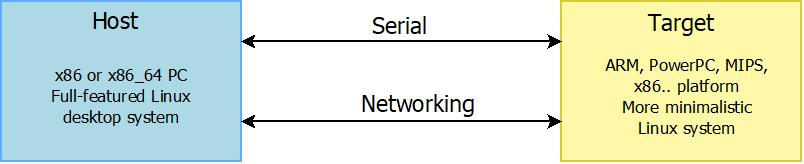
\includegraphics[width=0.7\textwidth]{slides/sysdev-dev-environment/host-vs-target.jpg}
  \end{center}
\end{frame}

\begin{frame}
  \frametitle{Serial line communication program}
  \begin{itemize}
  \item An essential tool for embedded development is a serial line
    communication program, like {\em HyperTerminal} in Windows.
  \item There are multiple options available in Linux: {\em Minicom},
    {\em Picocom}, {\em Gtkterm}, {\em Putty}, {\em screen}, {\em tmux}
    and the new {\em tio} (\url{https://github.com/tio/tio}).
  \item In this training session, we recommend using the simplest of
    them: {\em Picocom}
    \begin{itemize}
    \item Installation with \code{sudo apt install picocom}
    \item Run with \code{picocom -b BAUD_RATE /dev/SERIAL_DEVICE}.
    \item Exit with \code{[Ctrl][a] [Ctrl][x]}
    \end{itemize}
  \item \code{SERIAL_DEVICE} is typically
    \begin{itemize}
    \item \code{ttyUSBx} for USB to serial converters
    \item \code{ttySx} for real serial ports
    \end{itemize}
  \item Most frequent command: \code{picocom -b 115200 /dev/ttyUSB0}
  \end{itemize}
\end{frame}

\section{Cross-compiling toolchains}
\subsection{Definition and Components}

\begin{frame}
  \frametitle{Toolchain definition (1)}
  \begin{itemize}
  \item The usual development tools available on a GNU/Linux
    workstation is a {\bf native toolchain}
  \item This toolchain runs on your workstation and generates code for
    your workstation, usually x86
  \item For embedded system development, it is usually impossible or not
    interesting to use a native toolchain
    \begin{itemize}
    \item The target is too restricted in terms of storage and/or memory
    \item The target is very slow compared to your workstation
    \item You may not want to install all development tools on your target.
    \end{itemize}
  \item Therefore, {\bf cross-compiling toolchains} are generally
    used. They run on your workstation but generate code for your
    target.
  \end{itemize}
\end{frame}

\begin{frame}
  \frametitle{Toolchain definition (2)}
  \begin{center}
    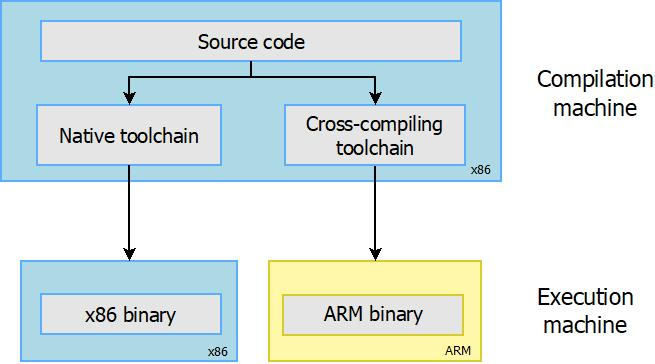
\includegraphics[width=0.8\textwidth]{slides/sysdev-toolchains-definition/cross-toolchain.jpg}
  \end{center}
\end{frame}

\begin{frame}{Architecture tuple and toolchain prefix}
  \begin{itemize}
  \item Many UNIX/Linux build mechanisms rely on {\em architecture
      tuple} names to identify machines.
  \item Examples: \code{arm-linux-gnueabihf},
    \code{mips64el-linux-gnu}, \code{arm-vendor-none-eabihf}
  \item These tuples are 3 or 4 parts:
    \begin{enumerate}
    \item The architecture name: \code{arm}, \code{riscv},
      \code{mips64el}, etc.
    \item Optionally, a vendor name, which is a free-form string
    \item An operating system name, or \code{none} when not targeting
      an operating system
    \item The ABI/C library (see later)
    \end{enumerate}
  \item This tuple is used to:
    \begin{itemize}
    \item configure/build software for a given platform
    \item as a prefix of cross-compilation tools, to differentiate
      them from the native toolchain
      \begin{itemize}
      \item \code{gcc} $\rightarrow$ native compiler
      \item \code{arm-linux-gnueabihf-gcc} $\rightarrow$ cross-compiler
      \end{itemize}
    \end{itemize}
  \end{itemize}
\end{frame}

\begin{frame}
  \frametitle{Components of gcc toolchains}
  \begin{center}
    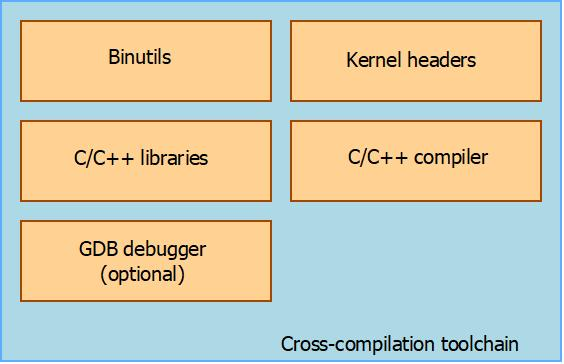
\includegraphics[width=0.8\textwidth]{slides/sysdev-toolchains-definition/components.jpg}
  \end{center}
\end{frame}

\begin{frame}
  \frametitle{Binutils}
  \begin{itemize}
  \item {\bf Binutils} is a set of tools to generate and manipulate
    binaries (usually with the ELF format) for a given CPU architecture
    \begin{itemize}
    \item \code{as}, the assembler, that generates binary code from
      assembler source code
    \item \code{ld}, the linker
    \item \code{ar}, \code{ranlib}, to generate \code{.a} archives
     (static libraries)
    \item \code{objdump}, \code{readelf}, \code{size}, \code{nm},
      \code{strings}, to inspect binaries. Very useful analysis tools!
    \item \code{objcopy}, to modify binaries
    \item \code{strip}, to strip parts of binaries that are just needed
      for debugging (reducing their size).
    \end{itemize}
  \item GNU Binutils: \url{https://www.gnu.org/software/binutils/}, GPL license
  \end{itemize}
\end{frame}

\begin{frame}
  \frametitle{C/C++ compiler}
  \begin{columns}
    \column{0.8\textwidth}
    \begin{itemize}
    \item GCC: GNU Compiler Collection, the famous free software compiler
    \item \url{https://gcc.gnu.org/}
    \item Can compile C, C++, Ada, Fortran, Java, Objective-C,
      Objective-C++, Go, etc. Can generate code for a large number of CPU
      architectures, including x86, ARM, RISC-V, and many others.
    \item Available under the GPL license, libraries under the GPL with
      linking exception.
    \end{itemize}
    \column{0.2\textwidth}
    
\includegraphics[width=0.7\textwidth]{slides/sysdev-toolchains-definition/gcc.png}
  \end{columns}
\end{frame}

\begin{frame}
  \frametitle{Kernel headers (1)}
  \begin{columns}
    \column{0.7\textwidth}
    \begin{itemize}
    \item The C standard library and compiled programs need to interact with the kernel
      \begin{itemize}
      \item Available system calls and their numbers
      \item Constant definitions
      \item Data structures, etc.
      \end{itemize}
    \item Therefore, compiling the C standard library requires kernel headers, and many
      applications also require them.
    \item Available in \code{<linux/...>} and \code{<asm/...>} and a few
      other directories corresponding to the ones visible in
      \kdir{include/uapi} and in \code{arch/<arch>/include/uapi} in the kernel sources
    \item The kernel headers are extracted from the kernel sources using
      the \code{headers_install} kernel Makefile target.
    \end{itemize}
    \column[c]{0.3\textwidth}
    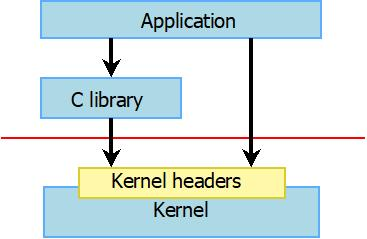
\includegraphics[width=\textwidth]{slides/sysdev-toolchains-definition/kernel-headers.jpg}
  \end{columns}
\end{frame}

\begin{frame}[fragile]
  \frametitle{Kernel headers (2)}
  \begin{itemize}
  \item System call numbers, in \code{<asm/unistd.h>}
\begin{verbatim}
#define __NR_exit         1
#define __NR_fork         2
#define __NR_read         3
\end{verbatim}
  \item Constant definitions, here in \code{<asm-generic/fcntl.h>},
    included from \code{<asm/fcntl.h>}, included from
    \code{<linux/fcntl.h>}
\begin{verbatim}
#define O_RDWR 00000002
\end{verbatim}
\item Data structures, here in \code{<asm/stat.h>} (used by the
\code{stat} command)
\begin{verbatim}
struct stat {
    unsigned long st_dev;
    unsigned long st_ino;
    [...]
};
\end{verbatim}
\end{itemize}
\end{frame}

\begin{frame}[fragile]
  \frametitle{Kernel headers (3)}
  The kernel to user space interface is {\bf backward compatible}
  \begin{itemize}
  \item Kernel developers are doing their best to {\bf never}
        break existing programs when the kernel is upgraded.
        Otherwise, users would stick to older kernels, which
        would be bad for everyone.
  \item Hence, binaries generated with a toolchain using kernel headers
        older than the running kernel will work without problem, but
        won't be able to use the new system calls, data structures, etc.
  \item Binaries generated with a toolchain using kernel headers
        newer than the running kernel might work only if they don't use
        the recent features, otherwise they will break.
  \end{itemize}
  What to remember: updating your kernel shouldn't break your programs;
  it's usually fine to keep an old toolchain as long is it works fine
  for your project.
\end{frame}

\begin{frame}
  \frametitle{C standard library}
  \begin{columns}
    \column{0.6\textwidth}
    \begin{itemize}
    \item The C standard library is an essential component of a Linux
          system.
      \begin{itemize}
      \item Interface between the applications and the kernel
      \item Provides the well-known standard C API to ease application
        development
      \end{itemize}
    \item Several C standard libraries are available:
      {\em glibc}, {\em uClibc}, {\em musl}, {\em klibc}, {\em
        newlib}...
    \item The choice of the C standard library must be made at
      cross-compiling toolchain generation time, as the GCC compiler is
      compiled against a specific C standard library.
    \end{itemize}
    \column{0.4\textwidth}
    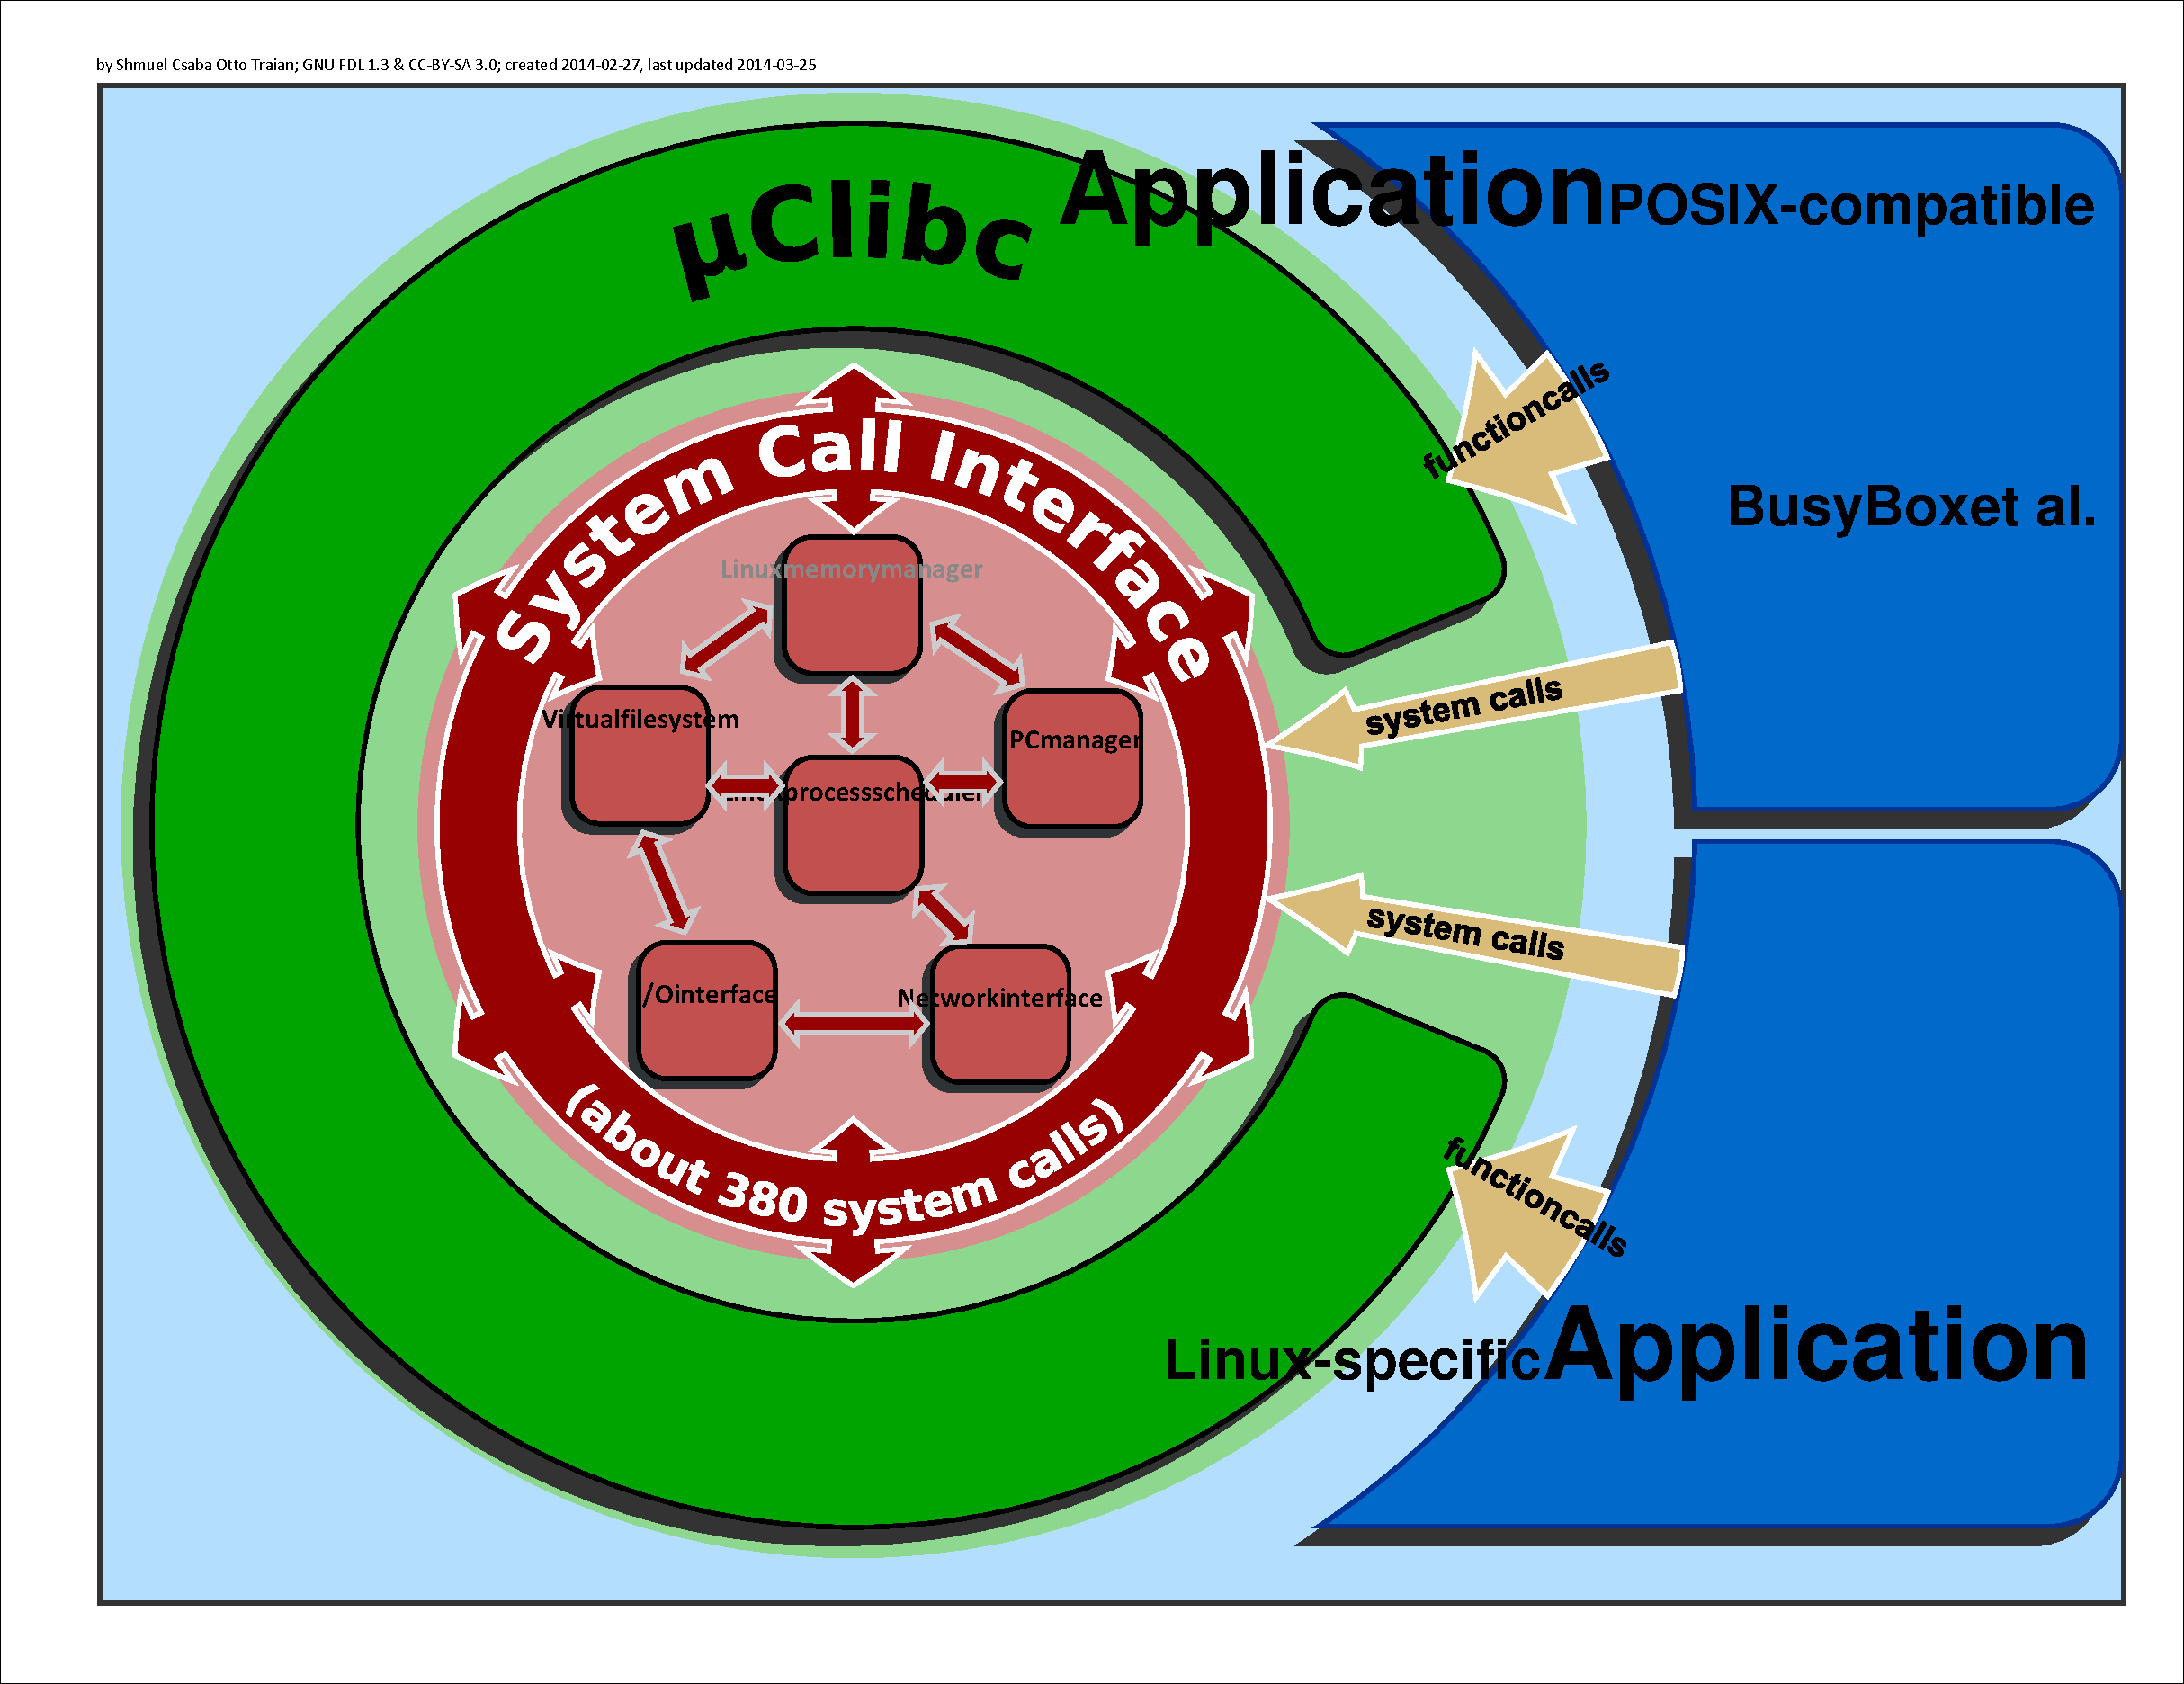
\includegraphics[width=\textwidth]{slides/sysdev-toolchains-definition/Linux_kernel_System_Call_Interface_and_uClibc.pdf}\\
    {\tiny Source: Wikipedia (\url{https://bit.ly/2zrGve2})}
  \end{columns}
\end{frame}

\begin{frame}
  \frametitle{glibc}
  \begin{columns}
    \column{0.7\textwidth}
    \begin{itemize}
    \item License: LGPL
    \item C standard library from the GNU project
    \item Designed for performance, standards compliance and portability
    \item Found on all GNU / Linux host systems
    \item Of course, actively maintained
    \item By default, quite big for small embedded systems.
      On armv7hf, version 2.31: \code{libc}: 1.5 MB, \code{libm}: 432
      KB, source: \url{https://toolchains.bootlin.com}
    \item \url{https://www.gnu.org/software/libc/}
    \end{itemize}
    \vfill
    \column{0.3\textwidth}
    \minipage[c][0.8\textheight][s]{\columnwidth}
    
\includegraphics[width=\textwidth]{slides/sysdev-toolchains-definition/heckert_gnu_white.pdf}
    \vfill
    \tiny \href{https://en.wikipedia.org/wiki/File:Heckert_GNU_white.svg}{Image source}
    \endminipage
  \end{columns}
\end{frame}

\begin{frame}
  \frametitle{uClibc-ng}
  \begin{itemize}
  \item \url{https://uclibc-ng.org/}
  \item A continuation of the old uClibc project, license: LGPL
  \item Lightweight C standard library for small embedded systems
    \begin{itemize}
    \item High configurability: many features can be enabled or
      disabled through a menuconfig interface.
    \item Supports most embedded architectures, including MMU-less
          ones (ARM Cortex-M, Blackfin, etc.). The only standard library
          supporting ARM noMMU.
    \item No guaranteed binary compatibility. May need to
      recompile applications when the library configuration changes.
    \item Some features may be implemented later than on glibc (real-time,
          floating-point operations...)
    \item Focus on size (RAM and storage) rather than performance
    \item Size on armv7hf, version 1.0.34:
      \code{libc}: 712 KB, source: \url{https://toolchains.bootlin.com}
    \end{itemize}
    \item Actively supported, supported by Buildroot but not by Yocto Project.
  \end{itemize}
\end{frame}

\begin{frame}
  \frametitle{musl C standard library}
  \begin{columns}
    \column{0.85\textwidth}
      \url{https://www.musl-libc.org/}
      \begin{itemize}
      \item A lightweight, fast and simple standard library for embedded systems
      \item Created while uClibc's development was stalled
      \item In particular, great at making small static executables,
	    which can run anywhere, even on a system built
            from another C standard library.
      \item More permissive license (MIT), making it easier to release
            static executables. We will talk about the requirements
            of the LGPL license (glibc, uClibc) later.
      \item Supported by build systems such as Buildroot and Yocto
        Project.
      \item Used by the Alpine Linux lightweight distribution
        (\url{https://www.alpinelinux.org/})
      \item Size on armv7hf, version 1.2.0:
        \code{libc}: 748 KB, source: \url{https://toolchains.bootlin.com}
      \end{itemize}
    \column{0.15\textwidth}
    
\includegraphics[width=\textwidth]{slides/sysdev-toolchains-definition/musl.png}
  \end{columns}
\end{frame}

\begin{frame}
  \frametitle{Other smaller C libraries}
  \begin{itemize}
  \item Several other smaller C libraries exist, but they do not
    implement the full POSIX interface required by most Linux
    applications
  \item They can run only relatively simple programs, typically to
    make very small static executables and run in very small root
    filesystems.
  \item Therefore not commonly used in most embedded Linux systems
  \item Choices:
    \begin{itemize}
    \item Newlib, \url{https://sourceware.org/newlib/}, maintained by
      Red Hat, used mostly in Cygwin, in bare metal and in small POSIX
      RTOS.
    \item Klibc, \url{https://en.wikipedia.org/wiki/Klibc}, from the
      kernel community, designed to implement small executables for
      use in an {\em initramfs} at boot time.
    \end{itemize}
  \end{itemize}
\end{frame}

\begin{frame}
  \frametitle{Advice for choosing the C standard library}
  \begin{itemize}
  \item Advice to start developing and debugging your applications
    with {\em glibc}, which is the most standard solution
  \item If you have size constraints, try to compile your app and then
    the entire filesystem with {\em uClibc} or {\em musl}
    \begin{itemize}
    \item The size advantage of {\em uClibc} or {\em musl}, which used
      to be a significant argument, is less relevant with today's
      storage capacities.
    \item Smaller binaries and filesystems remain useful when optimizing
      boot time, though, typically booting on a filesystem loaded in
      RAM, and to reduce the size of container and virtual machine images
      (one of the use cases of Alpine Linux).
    \end{itemize}
  \item If you run into trouble, it could be because of missing
    features in the C standard library.
  \item In case you wish to make static executables, {\em musl} will
    be an easier choice in terms of licensing constraints.
  \end{itemize}
\end{frame}

\begin{frame}{Linux vs. bare-metal toolchain}
  \begin{itemize}
  \item A {\bf Linux toolchain}
    \begin{itemize}
    \item is a toolchain that includes a Linux-ready C standard library, which
      uses the Linux system calls to implement system services
    \item can be used to build Linux user-space applications, but also
      bare-metal code (firmware, bootloader, Linux kernel)
    \item is identified by the \code{linux} OS identifier in the
      toolchain tuple: \code{arm-linux},
      \code{arm-none-linux-gnueabihf}
    \end{itemize}
  \item A {\bf bare metal toolchain}
    \begin{itemize}
    \item is a toolchain that does not include a C standard library, or a very
      minimal one that isn't tied to a particular operating
      system
    \item can be used to build only bare-metal code (firmware,
      bootloader, Linux kernel)
    \item is identified by the \code{none} OS identifier in the
      toolchain tuple: \code{arm-none-eabi}, \code{arm-none-none-eabi}
      (vendor is \code{none}, OS is \code{none})
    \end{itemize}
  \end{itemize}
\end{frame}

\begin{frame}{An alternate compiler suite: LLVM}
  \begin{itemize}
  \item Most Embedded Linux projects use toolchains based on GNU
    project: GCC compiler, binutils, GDB debugger
  \item The LLVM project has been developing an alternative compiler
    suite:
    \begin{itemize}
    \item Clang, C/C++ compiler, \url{https://clang.llvm.org/}
    \item LLDB, debugger, \url{https://lldb.llvm.org/}
    \item LLD, linker, \url{https://lld.llvm.org/}
    \item and more, see \url{https://llvm.org/}
    \end{itemize}
  \item While they are used by several high-profile projects, they are
    not yet in widespread use in most Embedded Linux projects.
  \item Initially had better code optimization and diagnostics than
    GCC, but thanks to having competition, GCC has improved
    significantly in this area.
  \item Available under MIT/BSD licenses
  \item \url{https://en.wikipedia.org/wiki/LLVM}
  \end{itemize}
\end{frame}

\subsection{Toolchain Options}
\begin{frame}
  \frametitle{ABI}
  \begin{itemize}
  \item When building a toolchain, the ABI used to generate binaries
    needs to be defined
  \item ABI, for {\em Application Binary Interface}, defines the
    calling conventions (how function arguments are passed, how the
    return value is passed, how system calls are made) and the
    organization of structures (alignment, etc.)
  \item All binaries in a system are typically compiled with the same ABI,
    and the kernel must understand this ABI.
  \item On ARM 32-bit, two main ABIs: {\em EABI} and {\em EABIhf}
    \begin{itemize}
    \item {\em EABIhf} passes floating-point arguments in
      floating-point registers $\rightarrow$ needs an ARM processor
      with a FPU
    \end{itemize}
  \item On RISC-V, several ABIs: {\em ilp32}, {\em ilp32f}, {\em ilp32d},
        {\em lp64}, {\em lp64f}, and {\em lp64d}
  \item {\fontsize{10}{15} \url{https://en.wikipedia.org/wiki/Application_Binary_Interface}}
  \end{itemize}
\end{frame}

\begin{frame}{Floating point support}
  \begin{itemize}
  \item All ARMv7-A (32-bit) and ARMv8-A (64-bit) processors have a
    floating point unit
  \item RISC-V cores with the \code{F} extension have a floating point
    unit
  \item Some older ARM cores (ARMv4/ARMv5) or some RISC-V cores may
    not have a floating point unit
  \item For processors without a floating point unit, two solutions
    for floating point computation:
    \begin{itemize}
    \item Generate {\em hard float code} and rely on the kernel to
      emulate the floating point instructions. This is very slow.
    \item Generate {\em soft float code}, so that instead of
      generating floating point instructions, calls to a user space
      library are generated
    \end{itemize}
  \item Decision taken at toolchain configuration time
  \item For processors with a floating point unit, sometimes different
    FPU are possible. For example on ARM: VFPv3, VFPv3-D16, VFPv4,
    VFPv4-D16, etc.
  \end{itemize}
\end{frame}

\begin{frame}
  \frametitle{CPU optimization flags}
  \begin{itemize}
  \item GNU tools (gcc, binutils) can only be compiled for a specific
        target architecture at a time (ARM, x86, RISC-V...)
  \item gcc offers further options:
    \begin{itemize}
    \item \code{-march} allows to select a specific target instruction set
    \item \code{-mtune} allows to optimize code for a specific CPU
    \item For example: \code{-march=armv7 -mtune=cortex-a8}
    \item \code{-mcpu=cortex-a8} can be used instead to allow gcc to infer the target
      instruction set (\code{-march=armv7}) and cpu optimizations (\code{-mtune=cortex-a8})
    \item \url{https://gcc.gnu.org/onlinedocs/gcc/ARM-Options.html}
    \end{itemize}
  \item At the GNU toolchain compilation time, values can be chosen. They are used:
    \begin{itemize}
    \item As the default values for the cross-compiling tools, when no
      other \code{-march}, \code{-mtune}, \code{-mcpu} options are
      passed
    \item To compile the C library
    \end{itemize}
  \item Note: LLVM (Clang, LLD...) utilities support multiple target architectures at once.
  \end{itemize}
\end{frame}

\subsection{Obtaining a Toolchain}

\begin{frame}
  \frametitle{Building a toolchain manually}

  \begin{itemize}
  \item Building a cross-compiling toolchain manually is a fairly
    difficult process
  \item Lots of details to learn: many components to build with
    complicated configuration
  \item Typical process is:
    \begin{itemize}
    \item Build dependencies of binutils/gcc (GMP, MPFR, ISL, etc.)
    \item Build {\em binutils}
    \item Build a baremetal, first stage {\em GCC}
    \item Extract kernel headers from the Linux source code
    \item Build the C library using the first stage GCC
    \item Build the second stage and final {\em GCC} supporting the Linux
          OS and the C library.
    \end{itemize}
  \item Many decisions to make about the components: C library, gcc
    and binutils versions, ABI, floating point mechanisms, etc. Not
    trivial to find correct combinations of these possibilities
  \item See the
    \href{https://crosstool-ng.github.io/docs/toolchain-construction/}{Crosstool-NG
      documentation} for details on how toolchains are built.
  \item Talk: {\em Anatomy of Cross-Compilation Toolchains}, by Thomas
    Petazzoni, ELCE 2017, \href{https://youtu.be/Pbt330zuNPc}{video} and
    \href{https://elinux.org/images/1/15/Anatomy_of_Cross-Compilation_Toolchains.pdf}{slides}
\end{itemize}
\end{frame}

\begin{frame}
  \frametitle{Get a pre-compiled toolchain}
  \begin{itemize}
  \item Solution that many people choose
    \begin{itemize}
    \item Advantage: it is the simplest and most convenient solution
    \item Drawback: you can't fine tune the toolchain to your needs
    \end{itemize}
  \item Make sure the toolchain you find meets your requirements: CPU,
    endianness, C library, component versions, version of the kernel
    headers, ABI, soft float or hard float, etc.
  \item Some possibilities:
    \begin{itemize}
    \item Toolchains packaged by your distribution, for example Ubuntu
      package
      \href{https://packages.ubuntu.com/gcc-arm-linux-gnueabihf}{gcc-arm-linux-gnueabihf}
      or Fedora
      \href{https://packages.fedoraproject.org/pkgs/cross-gcc/gcc-arm-linux-gnu/}{gcc-arm-linux-gnu}. Often
      limited to ARM/ARM64 with glibc.
    \item Bootlin's GNU toolchains, most CPU architectures, with
      glibc/uClibc/musl, \url{https://toolchains.bootlin.com}
    \item \href{https://developer.arm.com/tools-and-software/open-source-software/developer-tools/gnu-toolchain/downloads}
      {ARM and ARM64 toolchains released by ARM}
    \end{itemize}
  \end{itemize}
\end{frame}

\begin{frame}{Example of toolchains from ARM: downloading}
  \begin{columns}
    \column{0.6\textwidth}
    \begin{center}
      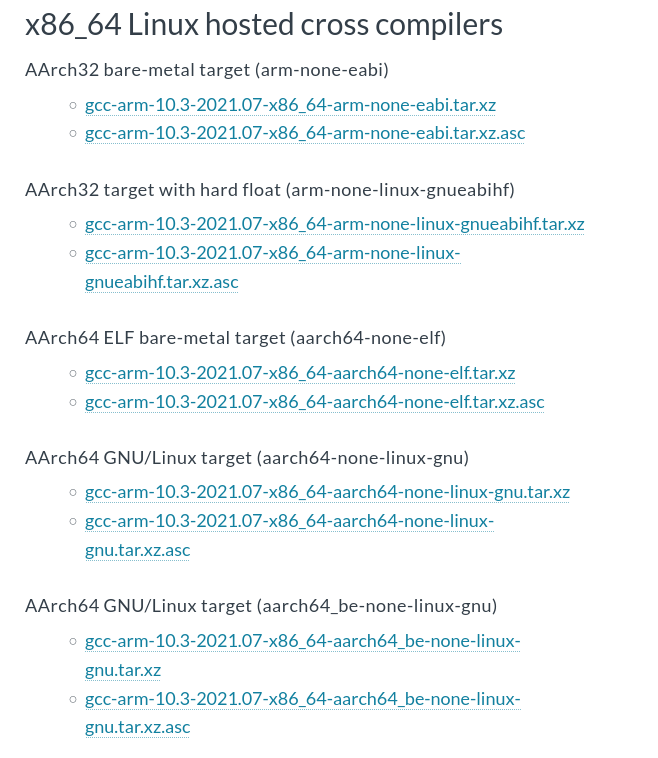
\includegraphics[height=0.8\textheight]{slides/sysdev-toolchains-obtaining/arm-toolchain.png}
    \end{center}
    \column{0.4\textwidth}
    From \href{https://developer.arm.com/tools-and-software/open-source-software/developer-tools/gnu-toolchain/downloads}
    {Arm GNU Toolchains}
  \end{columns}
\end{frame}

\begin{frame}[fragile]{Example of toolchains from ARM: using}
  \begin{block}{}
    {\tiny
\begin{verbatim}
$ wget https://developer.arm.com/-/media/Files/downloads/gnu-a/10.3-2021.07/binrel/[...]
    [...]gcc-arm-10.3-2021.07-x86_64-arm-none-linux-gnueabihf.tar.xz

$ tar xf gcc-arm-10.3-2021.07-x86_64-arm-none-linux-gnueabihf.tar.xz

$ cd gcc-arm-10.3-2021.07-x86_64-arm-none-linux-gnueabihf/

$ ./bin/arm-none-linux-gnueabihf-gcc -o test test.c

$ file test
test: ELF 32-bit LSB executable, ARM, EABI5 version 1 (SYSV), dynamically linked, interpreter /lib/ld-linux-armhf.so.3, [...]
   for GNU/Linux 3.2.0, with debug_info, not stripped
\end{verbatim}
    }
  \end{block}
\end{frame}

\begin{frame}
  \frametitle{Toolchain building utilities}
  Another solution is to use utilities that {\bf automate the process of
  building the toolchain}
  \begin{itemize}
  \item Same advantage as the pre-compiled toolchains: you don't need
    to mess up with all the details of the build process
  \item But also offers more flexibility in terms of toolchain
    configuration, component version selection, etc.
  \item Allows to rebuild the toolchain if needed to fix a bug or
    security issue.
  \item They also usually contain several patches that fix known
    issues with the different components on some architectures
  \item Multiple tools with identical principle: shell scripts or
    Makefile that automatically fetch, extract, configure, compile and
    install the different components
\end{itemize}
\end{frame}

\begin{frame}
  \frametitle{Toolchain building utilities (2)}
  \begin{columns}
  \column{0.6\textwidth}
    {\bf Crosstool-ng}
    \begin{itemize}
      \item Rewrite of the older Crosstool, with a menuconfig-like configuration
	system
      \item Feature-full: supports uClibc, glibc and musl,
            hard and soft float, many architectures
      \item Actively maintained
      \item \url{https://crosstool-ng.github.io/}
    \end{itemize}
  \column{0.4\textwidth}
    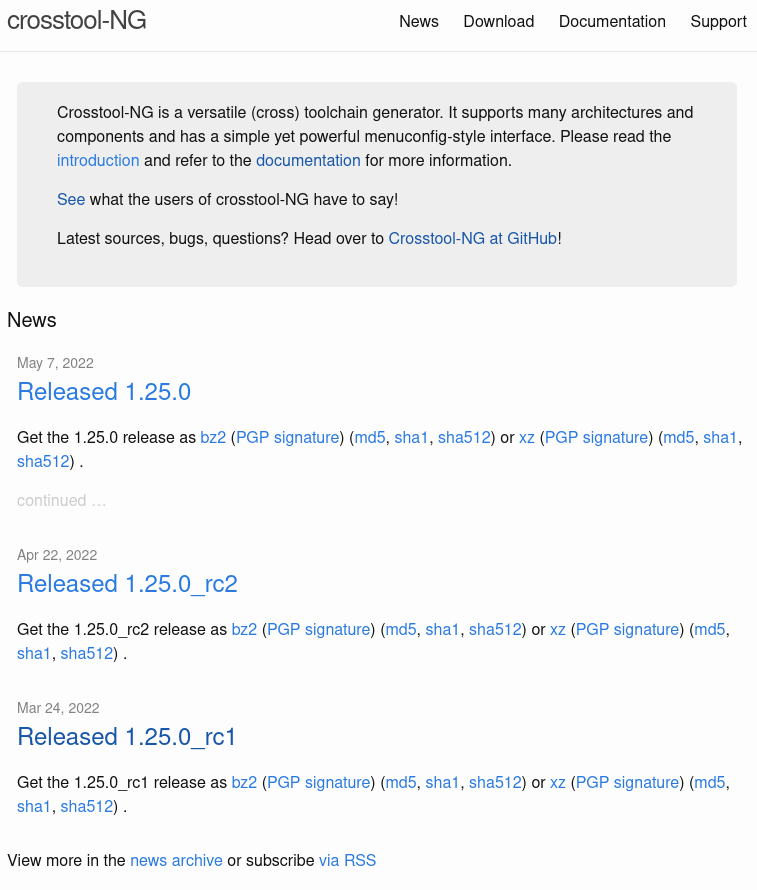
\includegraphics[width=\textwidth]{slides/sysdev-toolchains-obtaining/crosstool-ng.png}
  \end{columns}
\end{frame}

\begin{frame}
\frametitle{Toolchain building utilities (3)}
Many root filesystem build systems also allow the construction of
a cross-compiling toolchain
\begin{itemize}
\item {\bf Buildroot}
  \begin{itemize}
  \item Makefile-based. Can build glibc, uClibc and musl based
    toolchains, for a wide range of architectures. Use \code{make sdk}
    to only generate a toolchain.
  \item \url{https://buildroot.org}
  \end{itemize}
\item {\bf PTXdist}
  \begin{itemize}
  \item Makefile-based, maintained mainly by {\em Pengutronix},
        supporting only glibc and uClibc (version 2023.01 status)
  \item \url{https://www.ptxdist.org/}
  \end{itemize}
\item {\bf OpenEmbedded / Yocto Project}
  \begin{itemize}
  \item A featureful, but more complicated build system, supporting only
        glibc and musl.
  \item \url{https://www.openembedded.org/}
  \item \url{https://www.yoctoproject.org/}
  \end{itemize}
\end{itemize}
\end{frame}

\begin{frame}[fragile]{Crosstool-NG: download}
  \begin{itemize}
  \item Getting Crosstool-NG
\begin{verbatim}
$ git clone https://github.com/crosstool-ng/crosstool-ng.git
\end{verbatim}
  \item Using a well-known stable version
\begin{verbatim}
$ cd crosstool-ng
$ git checkout crosstool-ng-1.26.0
\end{verbatim}
  \item As we're fetching from Git, the \code{configure} script needs
    to be generated:
\begin{verbatim}
$ ./bootstrap
\end{verbatim}
  \end{itemize}
\end{frame}

\begin{frame}[fragile]{Crosstool-NG: installation}
  \begin{itemize}
  \item Installation can be done:
    \begin{itemize}
    \item system-wide, for example in \code{/usr/local}, the
      \code{ct-ng} command is then available globally
\begin{verbatim}
$ ./configure
$ make
$ sudo make install
\end{verbatim}
    \item or just locally in the source directory, the \code{ct-ng}
      command will be invoked from this directory
\begin{verbatim}
$ ./configure --enable-local
$ make
\end{verbatim}
    \end{itemize}
  \item In our labs, we will use the second method
  \item Note: the \code{make} invocation doesn't build any toolchain,
    it builds the \code{ct-ng} executable.
  \end{itemize}
\end{frame}

\begin{frame}{Crosstool-NG: toolchain configuration}
  \begin{itemize}
  \item Once installed, the \code{ct-ng} tool allows to configure and
    build an arbitrary number of toolchains
  \item Its configuration system is based on {\em kconfig}, like the
    Linux kernel configuration system
  \item Configuration of the toolchain to build stored in a
    \code{.config} file
  \item Example configurations provided with Crosstool-NG
    \begin{itemize}
    \item List: \code{./ct-ng list-samples}
    \item Load an example: \code{./ct-ng <sample-name>}, replaces \code{.config}
    \item For example \code{./ct-ng aarch64-unknown-linux-gnu}
    \item No sample loaded
      $\rightarrow$ default Crosstool-NG configuration is a bare-metal
      toolchain for the {\em Alpha} CPU architecture!
    \end{itemize}
  \item The configuration can then be refined using either:
    \begin{itemize}
    \item \code{./ct-ng menuconfig}
    \item \code{./ct-ng nconfig}
    \end{itemize}
  \end{itemize}
\end{frame}

\begin{frame}{Crosstool-NG: toolchain configuration}
  \begin{center}
    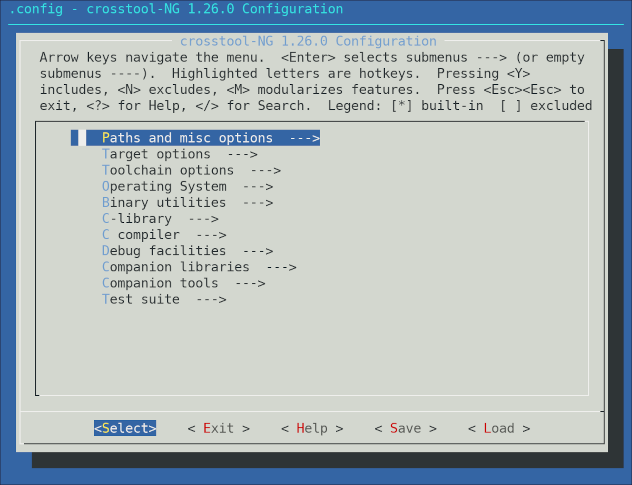
\includegraphics[height=0.7\textheight]{slides/sysdev-toolchains-obtaining/ct-ng-menu.png}
    \vspace{0.1cm}\\
    \code{./ct-ng menuconfig}
  \end{center}
\end{frame}

\begin{frame}[fragile]{Crosstool-NG: toolchain building}
  \begin{itemize}
  \item To build the toolchain
\begin{verbatim}
./ct-ng build
\end{verbatim}
    This will automatically download all the needed dependencies, and
    build all toolchain components in the right order, with the
    specified configuration.
  \item By default the results go in
    \code{$HOME/x-tools/<architecture-tuple>}, as defined by the
    option \code{CT_PREFIX_DIR} in {\em Paths and misc options}
  \end{itemize}
\end{frame}

\begin{frame}[fragile]{Important toolchain contents}
  \begin{itemize}
  \item \code{bin/}: cross compilation tool binaries
    \begin{itemize}
    \item This directory can be added to your \code{PATH} to ease
      usage of the toolchain
    \item Sometimes with symlinks for shorter names
\begin{verbatim}
arm-linux-gcc -> arm-cortexa7-linux-uclibcgnueabihf-gcc
\end{verbatim}
    \end{itemize}
  \item \code{<arch-tuple>/sysroot}: {\em sysroot} directory
    \begin{itemize}
    \item \code{<arch-tuple>/sysroot/lib}: C library, GCC runtime, C++
      standard library compiled for the target
    \item \code{<arch-tuple>/sysroot/usr/include}: C library headers
      and kernel headers
    \end{itemize}
  \end{itemize}
\end{frame}

\section{Bootloaders and firmware}
\subsection{Introduction}

\begin{frame}{Bootloader role}
  \begin{itemize}
  \item The bootloader is a piece of code responsible for
    \begin{itemize}
    \item Basic hardware initialization
    \item Loading of an application binary, usually an operating
      system kernel, from flash storage, from the network, or from
      another type of non-volatile storage.
    \item Possibly decompression of the application binary
    \item Execution of the application
    \end{itemize}
  \item Besides these basic functions, most bootloaders provide a
    shell or menu
    \begin{itemize}
    \item Menu to select the operating system to load
    \item Shell with commands to load data from storage or network,
      inspect memory, perform hardware testing/diagnostics
    \end{itemize}
  \item The first piece of code running by the processor that can be
    modified by us developers.
  \end{itemize}
\end{frame}

\subsection{Booting on x86 platforms}

\begin{frame}{Legacy BIOS booting (1)}
  \begin{itemize}
  \item x86 platforms shipped before 2005-2006 include a firmware
    called {\em BIOS}
    \begin{itemize}
    \item BIOS = Basic Input Output System
    \item Part of the hardware platform, closed-source, rarely
      modifiable
    \item Implements the booting process
    \item Provides runtime services that can be invoked - not commonly
      used
    \item Stored in some flash memory, outside of regular
      user-accessible storage devices
    \end{itemize}
  \item To be bootable, the first sector of a storage device is
    ``special''
    \begin{itemize}
    \item MBR = Master Boot Record
    \item Contains the partition table
    \item Contains up to 446 bytes of bootloader code, loaded into RAM
      and executed
    \item The BIOS is responsible for the RAM initialization
    \end{itemize}
  \item \url{https://en.wikipedia.org/wiki/BIOS}
  \end{itemize}
\end{frame}

\begin{frame}{Legacy BIOS booting (2)}
  \begin{itemize}
  \item Due to the limitation in size of the bootloader, bootloaders
    are split into two stages
    \begin{itemize}
    \item Stage 1, which fits within the 446 bytes constraint
    \item Stage 2, which is loaded by stage 1, and can therefore be
      bigger
    \end{itemize}
  \item Stage 2 is typically stored outside of any filesystem, at a
    fixed offset $\rightarrow$ simpler to load by stage 1
  \item Stage 2 generally has filesystem support, so it can load the
    kernel image from a filesystem
  \end{itemize}
\end{frame}

\begin{frame}{Legacy BIOS booting: sequence and storage}
  \begin{center}
    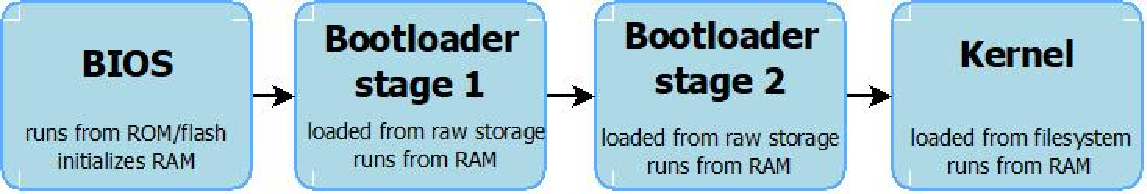
\includegraphics[width=0.7\textwidth]{slides/sysdev-bootloaders-sequence/legacy-bios-sequence.pdf}\\
    \vspace{0.5cm}
    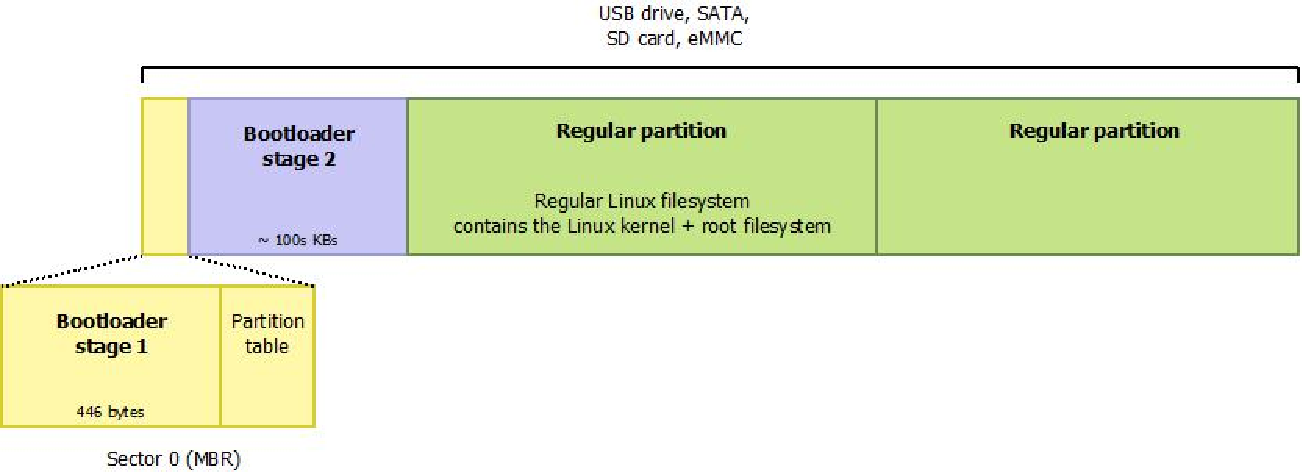
\includegraphics[width=0.9\textwidth]{slides/sysdev-bootloaders-sequence/legacy-bios-storage.pdf}
  \end{center}
\end{frame}

\begin{frame}{UEFI booting}
  \begin{itemize}
  \item Starting from 2005-2006, UEFI is the new firmware interface on
    x86 platforms
    \begin{itemize}
    \item Unified Extensible Firmware Interface
    \item Describes the interface between the operating system and the
      firmware
    \item Firmware in charge of booting
    \item Firmware also provides runtime services to the operating
      system
    \item Stored in some flash memory, outside of regular
      user-accessible storage devices
    \end{itemize}
  \item Loads EFI binaries from the {\em EFI System Partition}
    \begin{itemize}
    \item Generally a bootloader
    \item Can also be directly the Linux kernel, with an {\em EFI Boot
        Stub}
    \end{itemize}
  \item Special partition, formatted with the {\em FAT} filesystem
    \begin{itemize}
    \item MBR: identified by type \code{0xEF}
    \item GPT: identified with a specific {\em globally unique identifier}
    \end{itemize}
  \item File \code{/efi/boot/bootx32.efi}, \code{/efi/boot/bootx64.efi}
  \item \url{https://en.wikipedia.org/wiki/UEFI}
  \end{itemize}
\end{frame}

\begin{frame}{UEFI booting: sequence and storage}
  \begin{center}
    \vspace{0.5cm}
    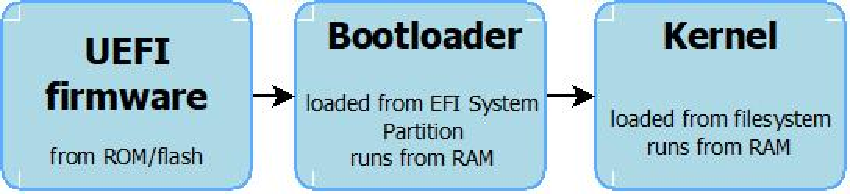
\includegraphics[width=0.7\textwidth]{slides/sysdev-bootloaders-sequence/uefi-sequence.pdf}\\
    \vspace{0.5cm}
    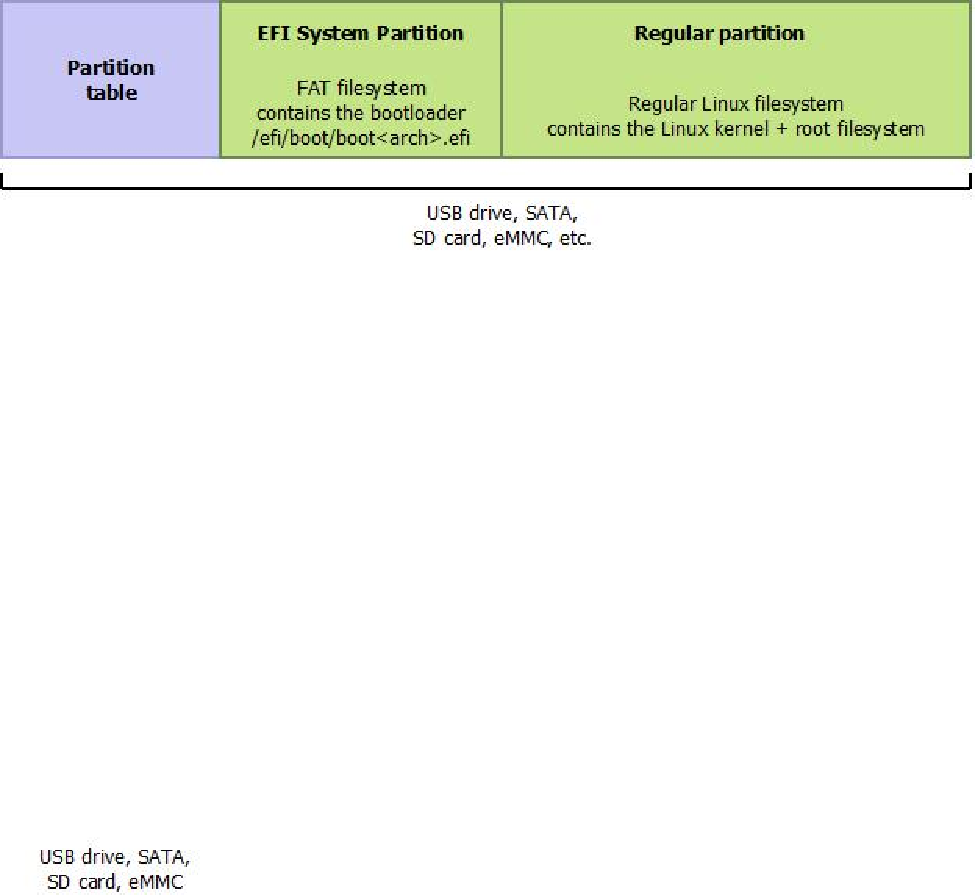
\includegraphics[width=0.9\textwidth]{slides/sysdev-bootloaders-sequence/uefi-storage.pdf}\\
  \end{center}
\end{frame}

\begin{frame}{ACPI}
  \begin{itemize}
  \item Advanced Configuration and Power Interface
  \item {\em Open standard that operating systems can use to discover
      and configure computer hardware components, to perform power
      management, to perform auto configuration, and to perform status
      monitoring}
  \item {\em Tables} with descriptions of the hardware that cannot be
    dynamically discovered at runtime
  \item Tables provided by the firmware (UEFI or legacy) and used by
    the operating system (Linux kernel in our case)
  \item \small \url{https://en.wikipedia.org/wiki/Advanced_Configuration_and_Power_Interface}
  \end{itemize}
\end{frame}

\begin{frame}{UEFI and ACPI on ARM}
  \begin{itemize}
  \item Historically UEFI and ACPI are technologies coming from the
    Intel/x86 world
  \item ARM is also pushing for the adoption of UEFI and ACPI as part
    of its {\em ARM System Ready} certification
    \begin{itemize}
    \item Mainly for servers/workstations SoCs
    \item Does not impact embedded SoCs
    \item Currently not common in embedded Linux projects on ARM
    \item \url{https://www.arm.com/architecture/system-architectures/systemready-certification-program}
    \end{itemize}
  \item Also some on-going effort to use UEFI on RISC-V, but not the
    de-facto standard
  \item When an embedded platform uses UEFI $\rightarrow$ its booting
    process is similar to an {\em x86} platform
  \end{itemize}
\end{frame}

\subsection{Booting on embedded platforms}

\begin{frame}{Booting on embedded platforms: ROM code}
  \begin{itemize}
  \item Most embedded processors include a {\bf ROM code} that
    implements the initial step of the boot process
  \item The ROM code is written by the processor vendor and directly
    built into the processor
    \begin{itemize}
    \item Cannot be changed or updated
    \item Its behavior is described in the processor datasheet
    \end{itemize}
  \item Responsible for finding a suitable bootloader, loading it and
    running it
    \begin{itemize}
    \item From NAND/NOR flash, from USB, from SD card, from eMMC, etc.
    \item Well defined location/format
    \end{itemize}
  \item {\em Generally} runs with the external RAM not initialized, so
    it can only load the bootloader into an internal SRAM
    \begin{itemize}
    \item Limited size of the bootloader, due to the size of the SRAM
    \item Forces the boot process to be split in two steps: first
      stage bootloader (small, runs from SRAM, initializes external DRAM),
      second stage bootloader (larger, runs from external DRAM)
    \end{itemize}
  \end{itemize}
\end{frame}

\begin{frame}{Booting on STM32MP1: datasheet}
  \begin{columns}
    \column{0.7\textwidth}
    \begin{center}
      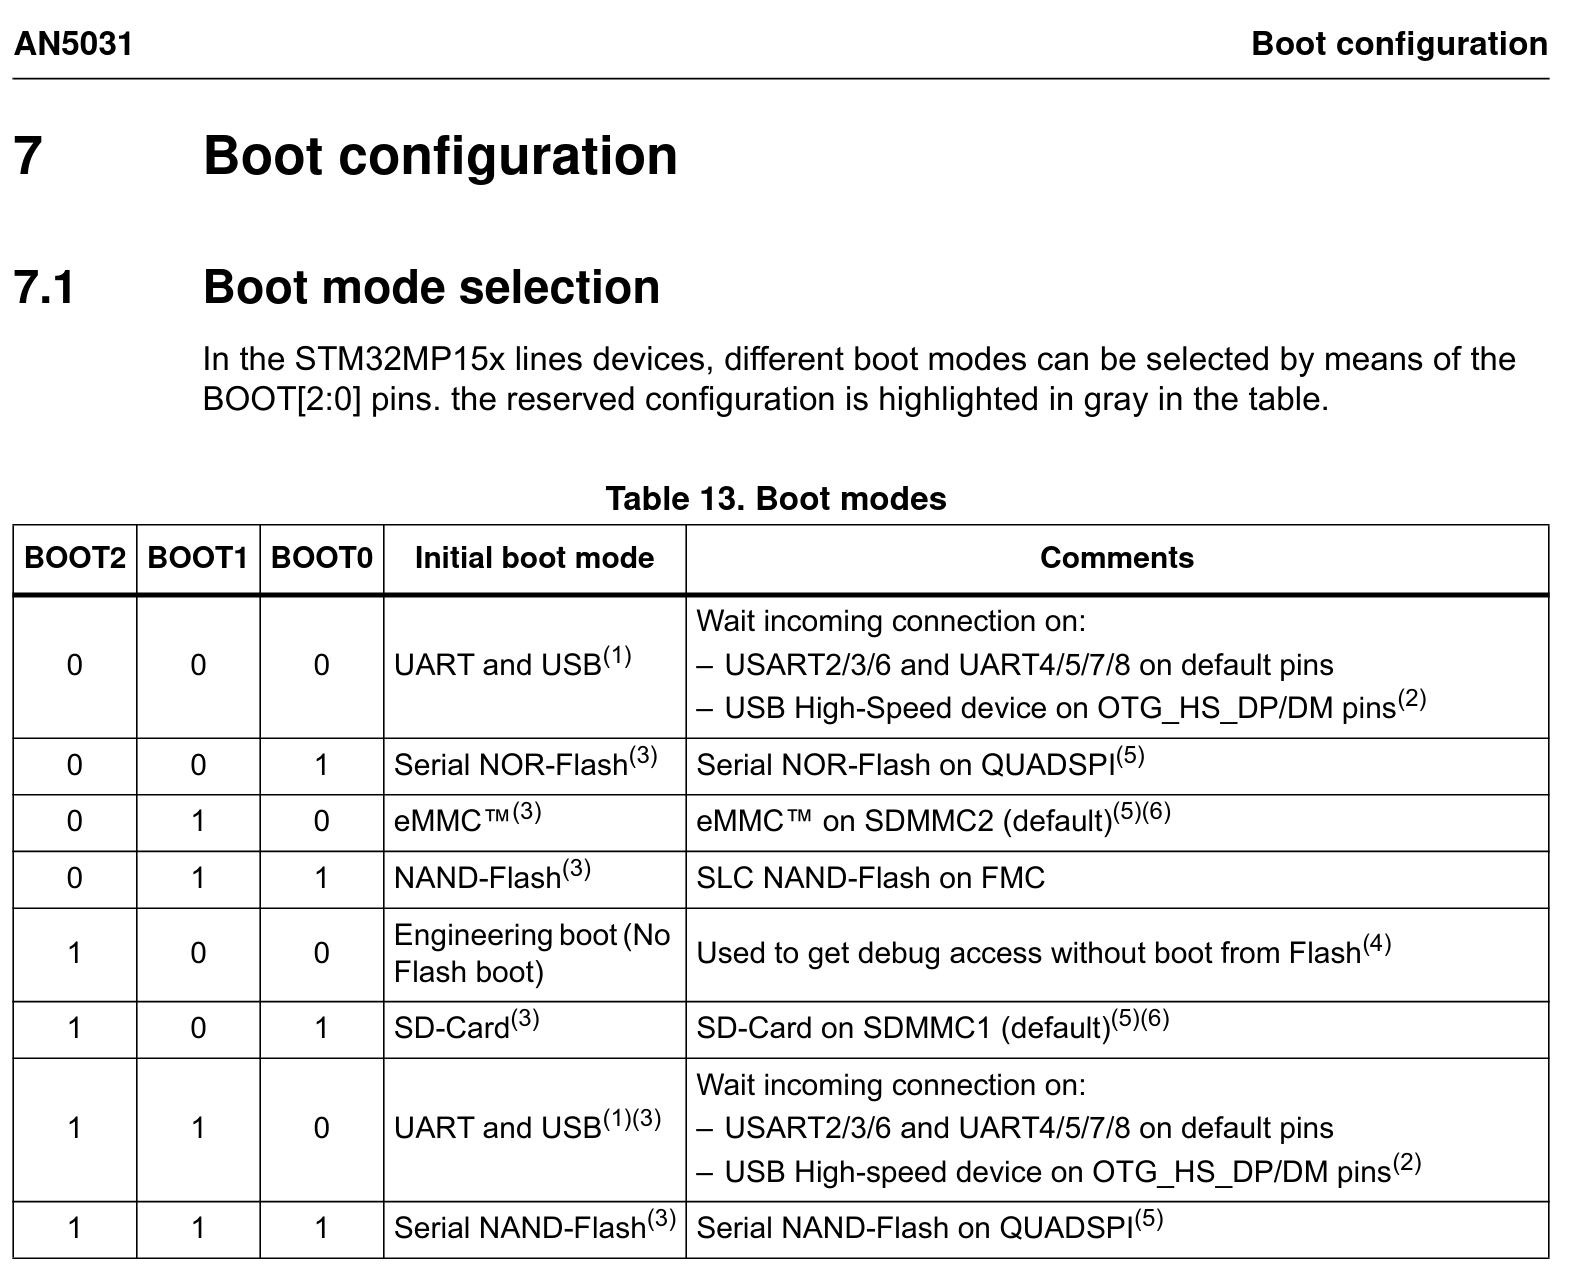
\includegraphics[height=0.85\textheight]{slides/sysdev-bootloaders-sequence/stm32mp1-rom-code.png}
    \end{center}
    \column{0.3\textwidth}
    {\tiny
      Source: \url{https://www.st.com/resource/en/application_note/dm00389996-getting-started-with-stm32mp151-stm32mp153-and-stm32mp157-line-hardware-development-stmicroelectronics.pdf}\\
      Useful details: \url{https://wiki.st.com/stm32mpu/wiki/STM32_MPU_ROM_code_overview}
    }
  \end{columns}
\end{frame}

\begin{frame}{Booting on AM335x (32 bit BeagleBone): datasheet}
  \begin{columns}
      \column{0.6\textwidth}
      \begin{center}
        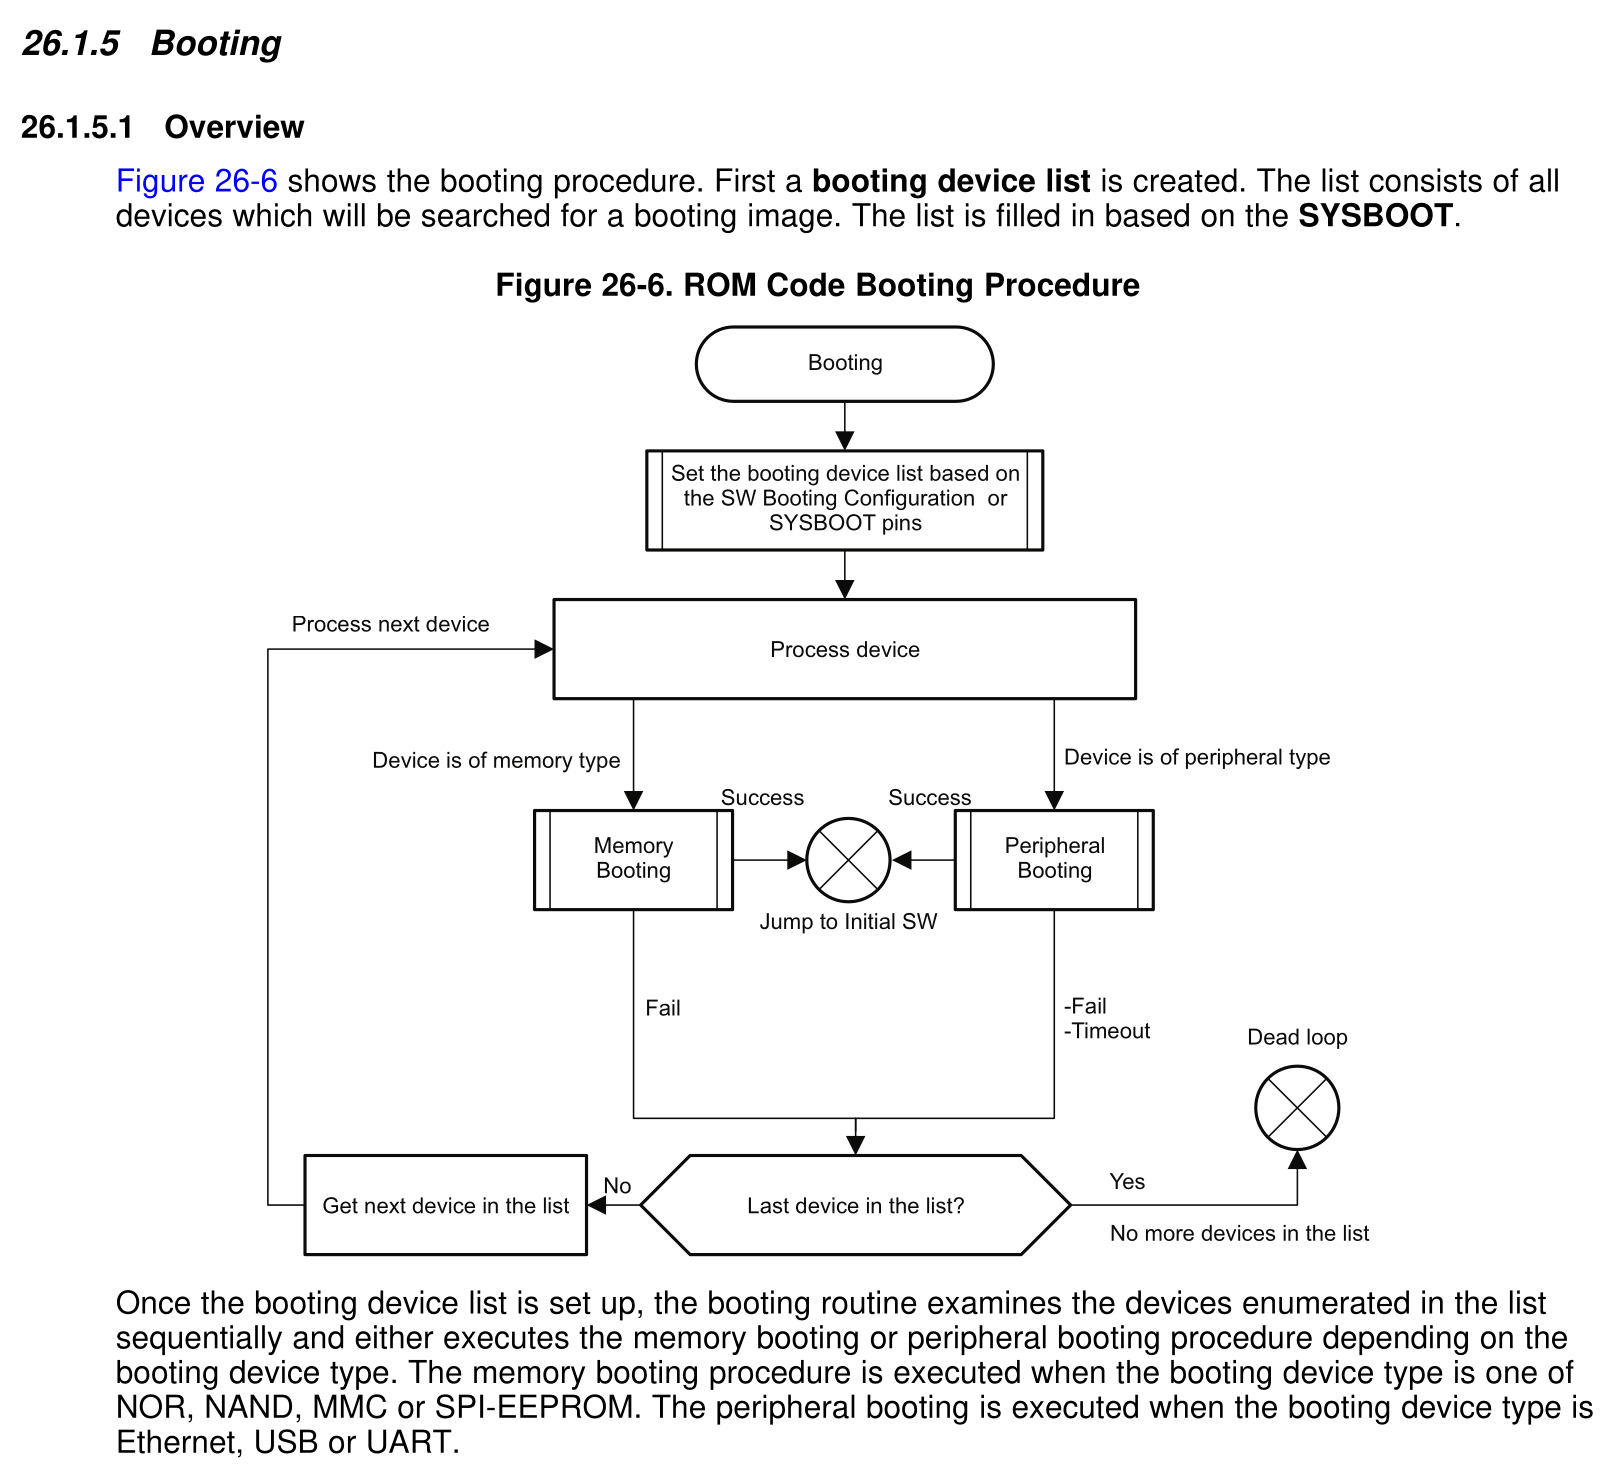
\includegraphics[height=0.85\textheight]{slides/sysdev-bootloaders-sequence/am335x-rom-code.png}
      \end{center}
      \column{0.4\textwidth}
      {\tiny
        Source:\\
        \url{https://www.mouser.com/pdfdocs/spruh73h.pdf},\\
	chapter 26
      }
    \end{columns}
\end{frame}

\begin{frame}{Two stage booting sequence}
  \begin{center}
    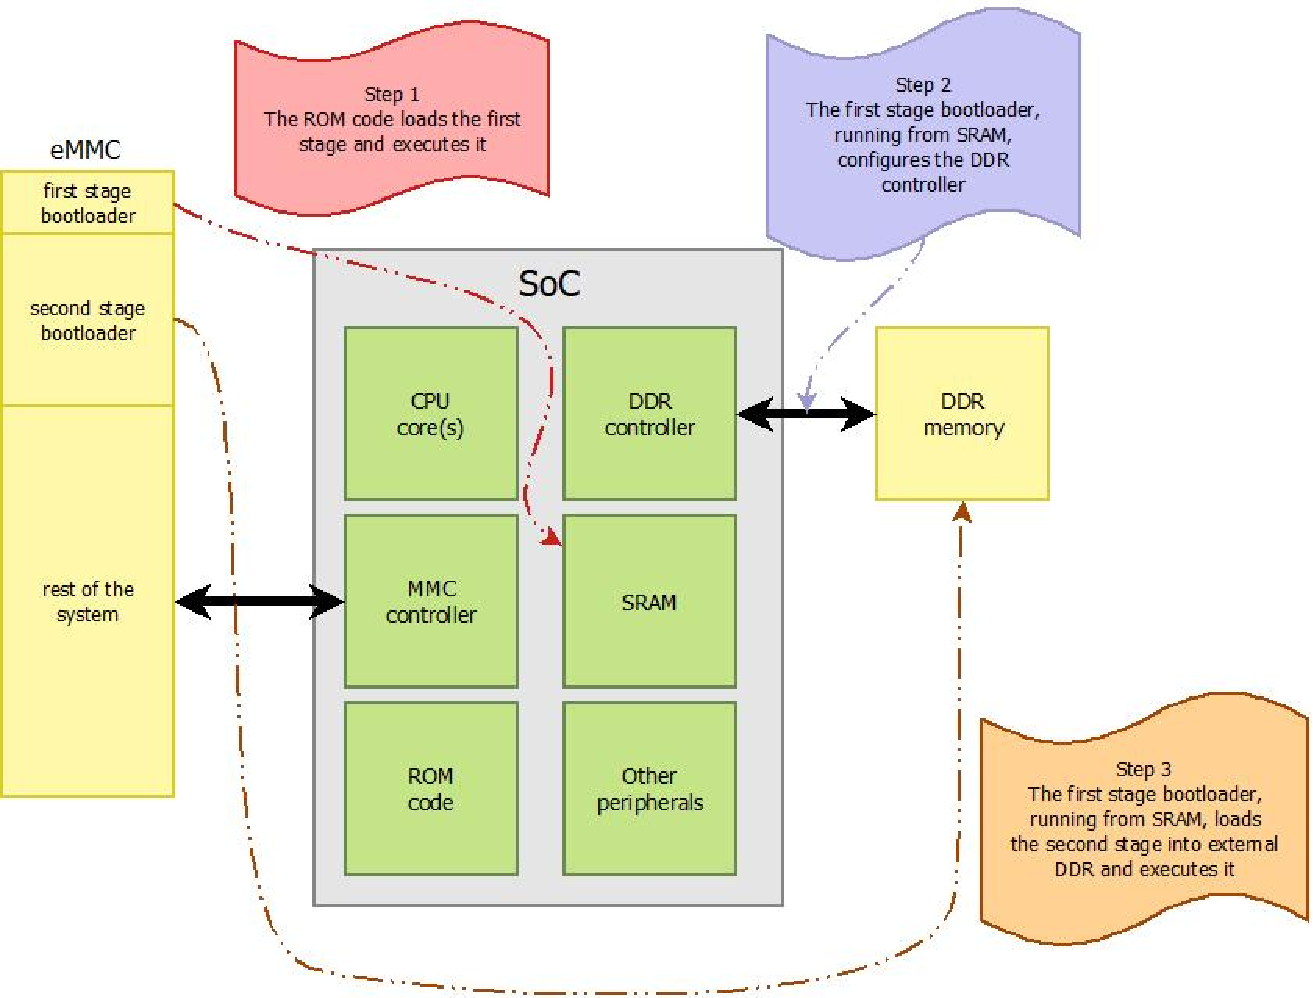
\includegraphics[height=0.85\textheight]{slides/sysdev-bootloaders-sequence/two-step-boot-process.pdf}
  \end{center}
\end{frame}

\begin{frame}{ROM code recovery mechanism}
  \begin{columns}
    \footnotesize
    \column{0.6\textwidth}
    \begin{itemize}
    \item Most ROM code also provide some sort of {\em recovery}
      mechanism, allowing to flash a board with no bootloader or a broken
      one, usually with a vendor-specific protocol over UART or USB.
    \item Often allows to push a new bootloader into RAM, making it
      possible to reflash the bootloader.
    \item Vendor-specific tools to run on the workstation
      \begin{itemize}
      \item STM32MP1: \href{https://www.st.com/en/development-tools/stm32cubeprog.html}{STM32 Cube Programmer}
      \item NXP i.MX: \href{https://github.com/NXPmicro/mfgtools}{uuu}
      \item Microchip AT91/SAM: \href{https://www.microchip.com/en-us/development-tool/SAM-BA-In-system-Programmer}{SAM-BA}
      \item Allwinner: \href{https://github.com/linux-sunxi/sunxi-tools}{sunxi-fel}
      \item Some open-source, some proprietary
      \end{itemize}
    \item Snagboot: new vendor agnostic tool replacing the above ones:
          \url{https://github.com/bootlin/snagboot}
    \end{itemize}
    \column{0.4\textwidth}
    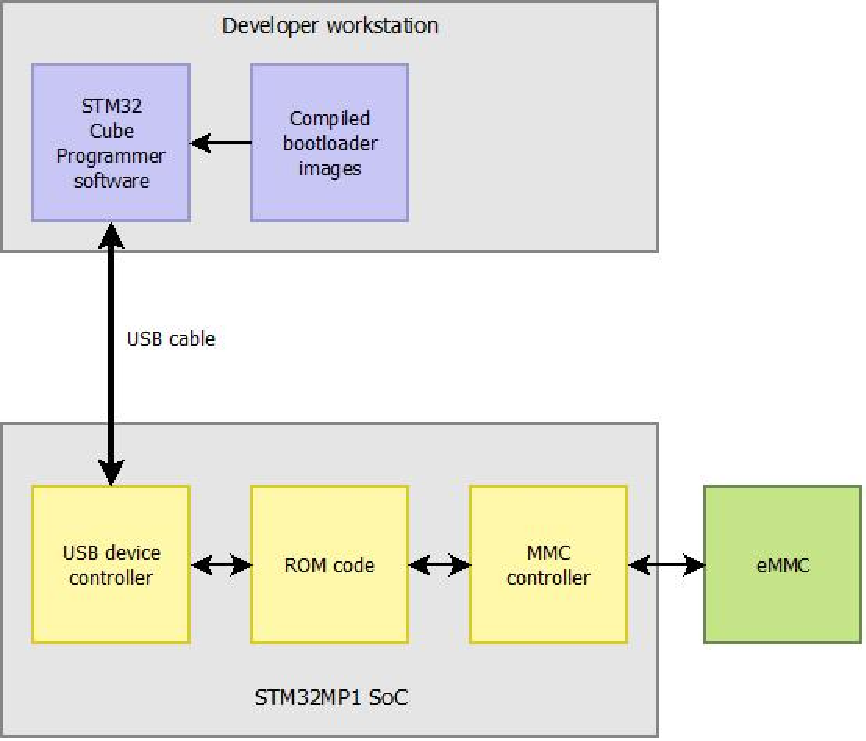
\includegraphics[width=\textwidth]{slides/sysdev-bootloaders-sequence/stm32mp1-rom-code-recovery.pdf}
  \end{columns}
\end{frame}

\subsection{Bootloaders}

\begin{frame}{GRUB}
  \begin{columns}
    \column{0.6\textwidth}
    \begin{itemize}
    \item {\em Grand Unified Bootloader}, from the GNU project
    \item De-facto standard in most Linux distributions for x86
      platforms
    \item Supports x86 legacy and UEFI systems
    \item Can read many filesystem formats to load the kernel image,
      modules and configuration
    \item Provides a menu and powerful shell with various commands
    \item Can load kernel images over the network
    \item Also supports ARM, ARM64, RISC-V, PowerPC, but less popular
      than other bootloaders on those platforms
    \item \url{https://www.gnu.org/software/grub/}
    \item \url{https://en.wikipedia.org/wiki/GNU_GRUB}
    \end{itemize}
    \column{0.4\textwidth}
    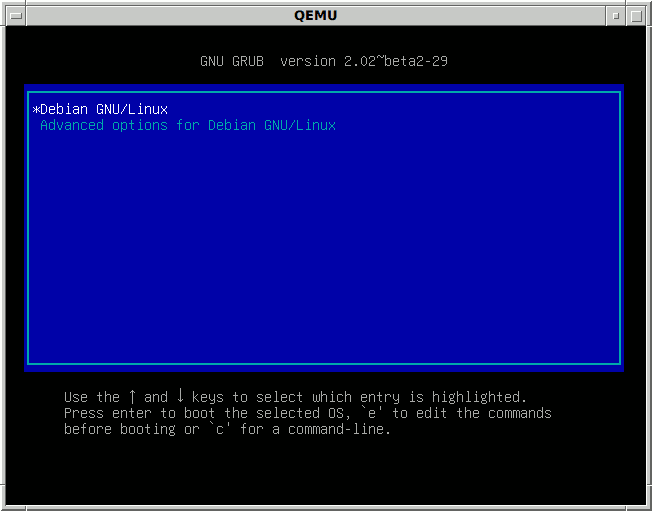
\includegraphics[width=\textwidth]{slides/sysdev-bootloaders-sequence/grub2.png}
  \end{columns}
\end{frame}

\begin{frame}{Syslinux}
  \begin{columns}
    \column{0.8\textwidth}
    \begin{itemize}
    \item For network and removable media booting (USB key, SD card, CD-ROM)
    \item \code{syslinux}: booting from FAT filesystem
    \item \code{pxelinux}: booting from the network
    \item \code{isolinux}: booting from CD-ROM
    \item \code{extlinux}: booting from numerous filesystem types
    \item A bit rustic to build and configure, not very actively
      maintained, but still useful for specific use-cases
    \item \url{https://wiki.syslinux.org/}
    \item \url{https://kernel.org/pub/linux/utils/boot/syslinux/}
    \end{itemize}
    \column{0.2\textwidth}
    
\includegraphics[width=\textwidth]{slides/sysdev-bootloaders-sequence/syslinux.png}
  \end{columns}
\end{frame}

\begin{frame}{systemd-boot}
  \begin{columns}
    \column{0.7\textwidth}
    \begin{itemize}
    \item Simple UEFI boot manager
    \item Useful alternative to GRUB for UEFI systems: simpler than GRUB
    \item Configured using files stored in the {\em EFI System
        Partition}
    \item Part of the {\em systemd} project, even though obviously
      distinct from {\em systemd} itself
      \begin{itemize}
      \item See our slides later in this course for more details on {\em
          systemd}
      \end{itemize}
    \item \url{https://www.freedesktop.org/wiki/Software/systemd/systemd-boot/}
    \end{itemize}
    \column{0.3\textwidth}
    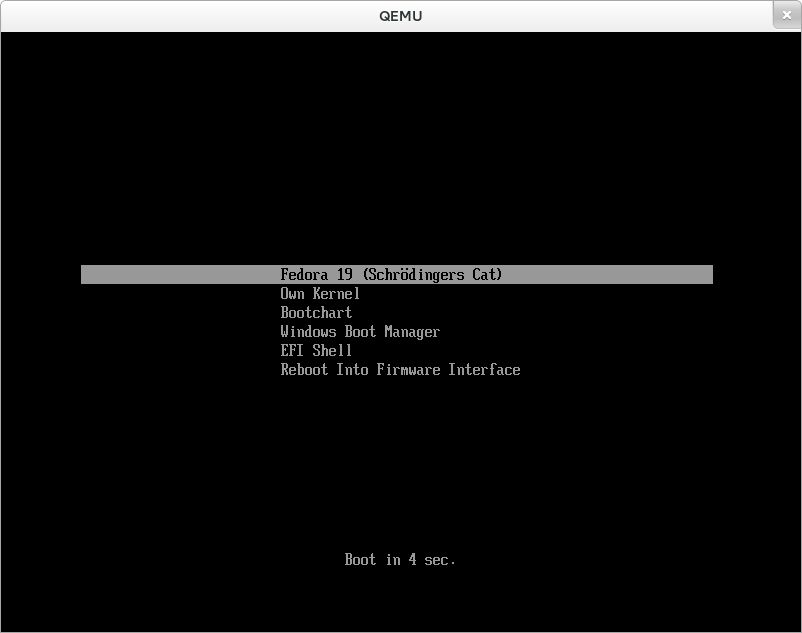
\includegraphics[width=\textwidth]{slides/sysdev-bootloaders-sequence/systemd-boot.png}
  \end{columns}
\end{frame}

\begin{frame}{shim}
  \begin{itemize}
  \item Minimal UEFI bootloader
  \item Mainly used in secure boot scenario: it is signed by Microsoft
    and therefore successfully verified by UEFI firmware in the field
  \item Allows to chainload another bootloader (GRUB) or directly
    the Linux kernel, with signature checking
  \item \url{https://github.com/rhboot/shim}
  \end{itemize}
\end{frame}

\begin{frame}{U-Boot}
  \begin{columns}
    \column{0.7\textwidth}
    \begin{itemize}
    \item The de-facto standard and most widely used bootloader on
      embedded architectures: ARM, ARM64, RISC-V, PowerPC, MIPS, and
      more.
    \item Also supports x86 with UEFI firmware.
    \item Very likely the one provided by your SoC vendor, SoM vendor
      or board vendor for your hardware.
    \item We will study it in detail in the next section, and use it in
      all practical labs of this course.
    \item \url{https://www.denx.de/wiki/U-Boot}
    \end{itemize}
    \column{0.3\textwidth}
    
\includegraphics[width=\textwidth]{slides/sysdev-bootloaders-sequence/u-boot.png}
  \end{columns}
\end{frame}

\begin{frame}{Barebox}
  \begin{columns}
    \column{0.7\textwidth}
    \begin{itemize}
    \item Another bootloader for most embedded CPU architectures:
      ARM/ARM64, MIPS, PowerPC, RISC-V, x86, etc.
    \item Initially developed as an alternative to U-Boot to address
      some U-Boot shortcomings
      \begin{itemize}
      \item {\em kconfig} for the configuration like the Linux kernel
      \item well-defined {\em device model} internally
      \item More Linux-style shell interface
      \item Cleaner code base
      \end{itemize}
    \item Actively maintained and developed, but
      \begin{itemize}
      \item Less widely used than U-Boot
      \item Less platform support than in U-Boot
      \end{itemize}
    \item \url{https://www.barebox.org/}
    \item Talk {\em barebox Bells and Whistles}, by Ahmad Fatoum, ELCE
      2020, \href{https://youtu.be/Oj7lKbFtyM0}{video} and
      \href{https://elinux.org/images/9/9d/Barebox-bells-n-whistles.pdf}{slides}
    \end{itemize}
    \column{0.3\textwidth}
    
\includegraphics[width=\textwidth]{slides/sysdev-bootloaders-sequence/barebox.png}
  \end{columns}
\end{frame}

\subsection{Trusted firmware}

\begin{frame}{Concept}
  \begin{itemize}
  \item Traditionally, bootloaders are only used during the booting
    process
    \begin{itemize}
    \item Bootloader loads operating system, jumps to it, and is
      discarded
    \end{itemize}
  \item Modern SoCs have advanced security mechanisms that require
    running some sort of {\em trusted firmware}
  \item This firmware is loaded by the bootloader, or part of the boot
    chain itself
  \item This {\em trusted firmware} {\bf stays resident} after control
    has been passed to the OS
    \begin{itemize}
    \item It is stored in a dedicated portion of the DDR, or some
      specific SRAM, inaccessible from the OS
    \item It provides services to the OS, which the OS cannot perform
      directly
    \item Can also be responsible for running a secure OS alongside the
      regular OS (Linux in our case)
    \end{itemize}
  \end{itemize}
\end{frame}

\begin{frame}{ARM}
  \begin{itemize}
  \item Modern ARMv7 and ARMv8 processors have
    \begin{itemize}
    \item 4 privilege levels ({\em Exception Levels})
      \begin{itemize}
      \item EL3, the most priviledged, runs secure firmware
      \item EL2, typically used by hypervisors, for virtualization
      \item EL1, used to run the Linux kernel
      \item EL0, used to run Linux user-space applications
      \end{itemize}
    \item 2 {\em worlds}
      \begin{itemize}
      \item Normal world, used to run a general purpose OS, like Linux
      \item Secure world, to run a separate, isolated, secure
        operating system and applications. Also called {\em TrustZone}
        by ARM.
      \end{itemize}
    \end{itemize}
  \item EL3 only exists in the secure world
  \item EL2 exists in both secure and normal worlds since ARMv8.4,
    before that EL2 was only in the normal world
  \item EL1 and EL0 exist in both secure and normal worlds
  \end{itemize}
\end{frame}

\begin{frame}{ARM exception levels and worlds}
  \begin{center}
    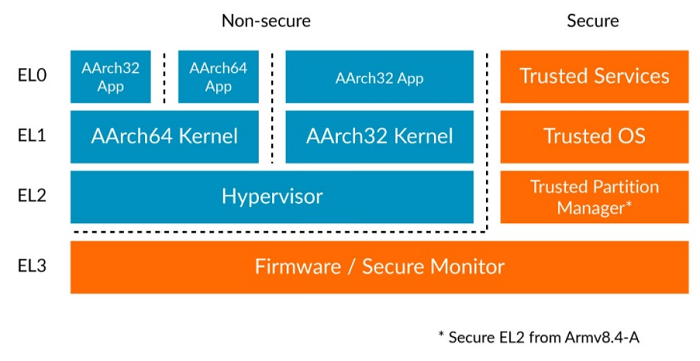
\includegraphics[height=0.75\textheight]{slides/sysdev-bootloaders-sequence/arm-exception-levels.png}
  \end{center}
  Source: \href{https://developer.arm.com/documentation/102412/0102/Execution-and-Security-states}{ARM documentation}
\end{frame}

\begin{frame}{Interfaces with secure firmware}
  \begin{columns}
    \column{0.8\textwidth}
    \begin{itemize}
    \item Standardized by ARM
    \item Services
      \begin{itemize}
      \item implemented by the secure firmware
      \item called by the operating system
      \end{itemize}
    \item Prevents the operating system running in normal world from
      directly accessing critical hardware resources
    \item
      \href{http://infocenter.arm.com/help/topic/com.arm.doc.den0022d/Power_State_Coordination_Interface_PDD_v1_1_DEN0022D.pdf}{PSCI},
      Power State Coordination Interface
      \begin{itemize}
      \item Power management related: turn CPUs on/off, CPU idle state,
        platform shutdown/reset
      \end{itemize}
    \item
      \href{http://infocenter.arm.com/help/topic/com.arm.doc.den0056a/DEN0056A_System_Control_and_Management_Interface.pdf}{SCMI},
      System Control and Management Interface
      \begin{itemize}
      \item Power domain, clocks, sensor, performance
      \end{itemize}
    \item Secure firmware implementing these interfaces is
      \begin{itemize}
      \item Mandatory to run Linux on ARMv8
      \item Mandatory to run Linux on some ARMv7 platforms, but not all
      \end{itemize}
    \end{itemize}
    \column{0.2\textwidth}
    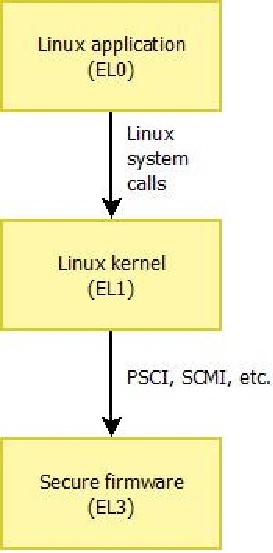
\includegraphics[width=\textwidth]{slides/sysdev-bootloaders-sequence/arm-interfaces.pdf}
  \end{columns}
\end{frame}

\begin{frame}{TF-A}
  \begin{itemize}
  \item {\em Trusted Firmware-A (TF-A) provides a reference
      implementation of secure world software for Armv7-A and Armv8-A,
      including a Secure Monitor executing at Exception Level 3 (EL3)}
  \item Formerly known as {\em ATF}, for ARM Trusted Firmware
  \item Implements the various standard interfaces that operating
    systems need from the secure firmware
  \item Has drivers for the hardware blocks that are not accessed
    directly by Linux
  \item Needs to be ported for each SoC
  \item Depending on the platform, may also need to be ported per
    board: DDR initialization
  \item Used on the vast majority of ARMv8 platforms, and on a few
    recent ARMv7 platforms
  \item \url{https://www.trustedfirmware.org/projects/tf-a/}
  \end{itemize}
\end{frame}

\begin{frame}{Trusted OS, OP-TEE}
  \begin{itemize}
  \item A trusted operating system can run in the {\em secure world},
    also called {\em Trusted Execution Environment} or {\em TEE}
  \item Hardware partitioning between {\em secure world} and {\em
      normal world}
    \begin{itemize}
    \item Some hardware resources only available in the {\em secure
        world}, by the trusted OS
    \end{itemize}
  \item Allows to run trusted applications/services
    \begin{itemize}
    \item isolated from Linux
    \item can provide services to Linux applications
    \end{itemize}
  \item Most common open-source implementation: {\em OP-TEE}
    \begin{itemize}
    \item Supported by most silicon vendors
    \item \url{https://www.op-tee.org/}
    \end{itemize}
  \end{itemize}
\end{frame}

\begin{frame}{ARM: summary}
  \begin{center}
    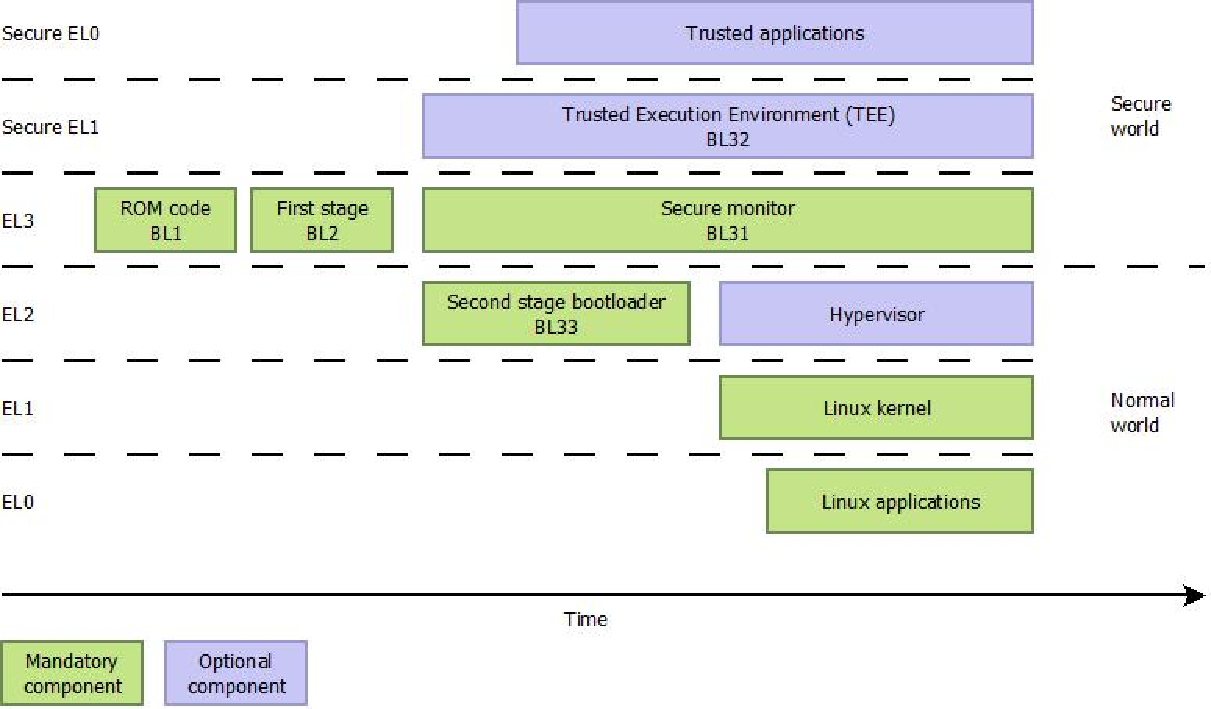
\includegraphics[height=0.70\textheight]{slides/sysdev-bootloaders-sequence/arm-nomenclature.pdf}
  \end{center}
  {\small Largely inspired from {\em Ahmad Fatoum} presentation
    {\em From Reset Vector to Kernel},
    \href{https://archive.fosdem.org/2021/schedule/event/from_reset_vector_to_kernel/attachments/slides/4632/export/events/attachments/from_reset_vector_to_kernel/slides/4632/from_reset_vector_to_kernel.pdf}{slides},
    \href{https://www.youtube.com/watch?v=-Ak9MWGxd7M}{video}}\\
    See also
    \href{https://trustedfirmware-a.readthedocs.io/en/latest/design/firmware-design.html}
    {details about the ARM terms: BL1, BL2...}
\end{frame}

\begin{frame}{RISC-V}
  \begin{columns}
    \column{0.7\textwidth}
    \begin{itemize}
    \item Linux-class RISC-V processors have several privilege levels
      \begin{itemize}
      \item M-mode: machine mode
      \item S-mode: level at which the Linux kernel runs
      \item U-mode: level at which Linux user-space
        applications run
      \end{itemize}
    \item Some specific HW resources are not accessible in S-mode
    \item A more priviledged firmware runs in M-mode
    \item RISC-V has defined SBI, {\em Supervisor Binary Interface}
      \begin{itemize}
      \item Standardized interface between the OS and the firmware
      \item \url{https://github.com/riscv-non-isa/riscv-sbi-doc}
      \end{itemize}
    \item OpenSBI is a reference, open-source implementation of SBI
      \begin{itemize}
      \item \url{https://github.com/riscv-software-src/opensbi}
      \end{itemize}
    \end{itemize}
    \column{0.3\textwidth}
    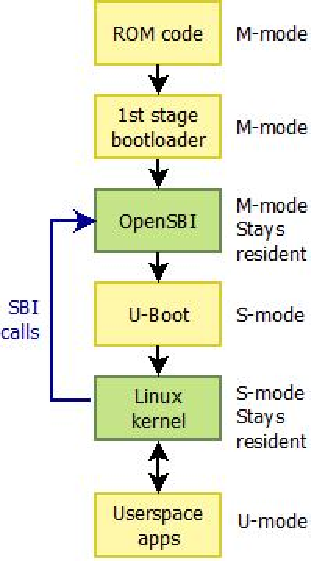
\includegraphics[width=\textwidth]{slides/sysdev-bootloaders-sequence/riscv-boot.pdf}
  \end{columns}
\end{frame}

\subsection{Example boot sequences on ARM}

\begin{frame}{TI AM335x (32 bit BeagleBone): ARMv7}
  \begin{center}
    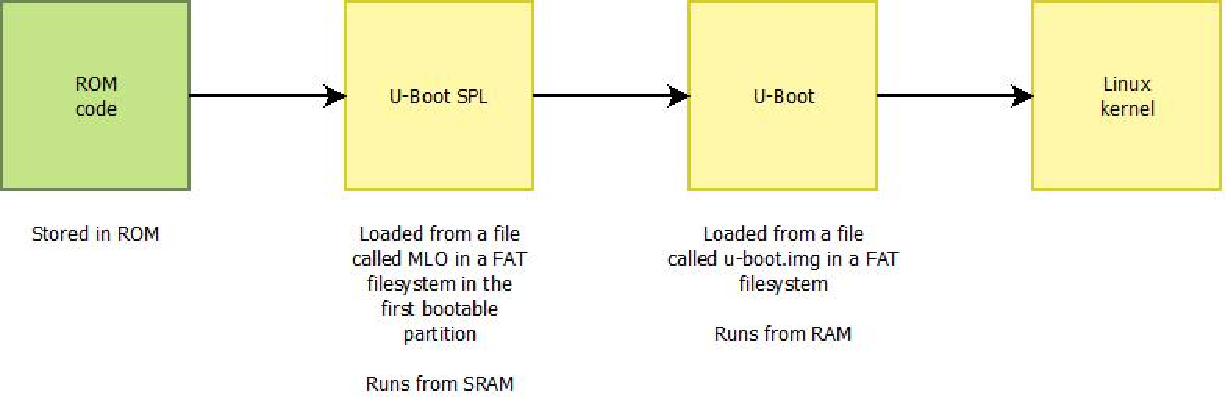
\includegraphics[width=\textwidth]{slides/sysdev-bootloaders-sequence/sequence-am335x.pdf}
  \end{center}
\end{frame}

\begin{frame}{NXP i.MX6: ARMv7}
  \begin{center}
    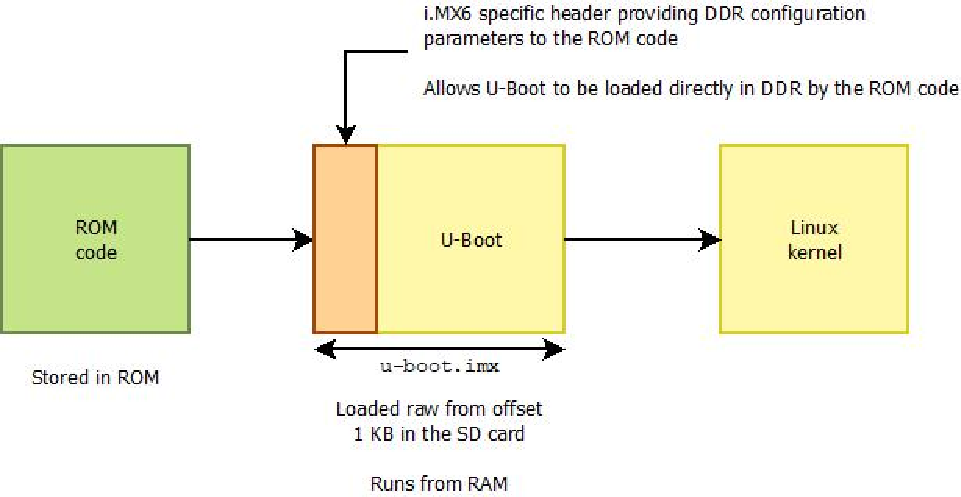
\includegraphics[height=0.7\textheight]{slides/sysdev-bootloaders-sequence/sequence-imx.pdf}
  \end{center}
  \vspace{0.1cm}
  Note: this diagram shows one possible boot flow on NXP i.MX6, but it
  is also possible to use the U-Boot SPL $\rightarrow$ U-Boot boot
  flow on i.MX6.
\end{frame}

\begin{frame}{STM32MP1: ARMv7}
  \begin{center}
    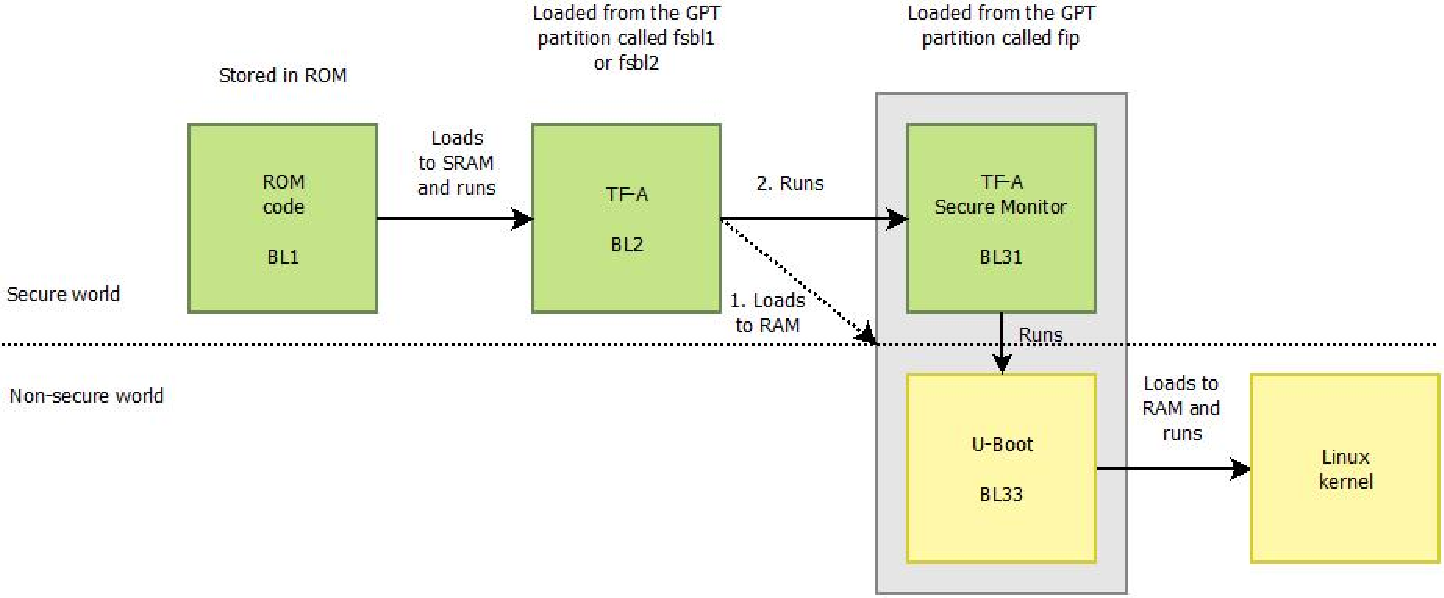
\includegraphics[width=\textwidth]{common/sequence-stm32mp1.pdf}
  \end{center}
  \vspace{0.3cm}
  Note: booting with U-Boot SPL and U-Boot is also possible.
\end{frame}

\begin{frame}{Allwinner ARMv8 cores}
  \begin{center}
    \includegraphics[height=0.8\textheight]{slides/sysdev-bootloaders-sequence/sequence-allwinner-64-bit.pdf}
  \end{center}
\end{frame}

\begin{frame}{TI AM62x (BeaglePlay): ARMv7 and ARMv8 cores}
  \begin{center}
    \includegraphics[height=0.8\textheight]{slides/sysdev-bootloaders-sequence/sequence-am62x.pdf}\\
    \footnotesize See \url{https://u-boot.readthedocs.io/en/latest/board/ti/am62x_sk.html} for details.
  \end{center}
\end{frame}

\section[Kernel]{Linux kernel introduction}

\ifthenelse{\equal{\training}{linux-kernel}}{
  \begin{frame}
  \frametitle{Origin}
  \begin{columns}
    \column{0.8\textwidth}
    \begin{itemize}
    \item The Linux kernel was created as a hobby in 1991 by a Finnish
      student, Linus Torvalds.
      \begin{itemize}
      \item Linux quickly started to be used as the kernel for free
        software operating systems
      \end{itemize}
    \item Linus Torvalds has been able to create a large and dynamic
      developer and user community around Linux.
    \item As of today, about 2,000+ people contribute to each kernel
      release, individuals or companies big and small.
    \end{itemize}
    \column{0.2\textwidth}
      \includegraphics[width=\textwidth]{slides/sysdev-linux-intro-features/linus-torvalds.jpg}
      \scriptsize
      Linus Torvalds in 2014\\
      \tiny
      Image credits (Wikipedia):\\
      \url{https://bit.ly/2UIa1TD}
    \end{columns}
\end{frame}
}{}

\begin{frame}
  \frametitle{Linux kernel in the system}
  \begin{center}
    \includegraphics[height=0.8\textheight]{slides/sysdev-linux-intro-features/linux-kernel-in-system.pdf}
  \end{center}
\end{frame}

\begin{frame}{Linux kernel main roles}
  \begin{itemize}
  \item {\bf Manage all the hardware resources}: CPU, memory, I/O.
  \item Provide a {\bf set of portable, architecture and hardware
      independent APIs} to allow user space applications and libraries
    to use the hardware resources.
  \item {\bf Handle concurrent accesses and usage} of hardware
    resources from different applications.
    \begin{itemize}
    \item Example: a single network interface is used by multiple
      user space applications through various network connections. The
      kernel is responsible for ``multiplexing'' the hardware resource.
    \end{itemize}
  \end{itemize}
\end{frame}

\begin{frame}
  \frametitle{System calls}
  \begin{columns}
    \column{0.7\textwidth}
    \begin{itemize}
    \item The main interface between the kernel and user space is the set
      of system calls
    \item About 400 system calls that provide the main kernel services
      \begin{itemize}
      \item File and device operations, networking operations,
        inter-process communication, process management, memory mapping,
        timers, threads, synchronization primitives, etc.
      \end{itemize}
      \ifthenelse{\equal{\training}{linux-kernel}}{}{
      \item This interface is stable over time: only new system calls can
        be added by the kernel developers
      }
    \item This system call interface is wrapped by the C library, and
      user space applications usually never make a system call directly
      but rather use the corresponding C library function
    \end{itemize}
    \column{0.3\textwidth}
      \includegraphics[width=\textwidth]{slides/sysdev-linux-intro-features/system-calls.pdf}
      \scriptsize
      Image credits (Wikipedia):\\
      \url{https://bit.ly/2U2rdGB}
    \end{columns}
\end{frame}

\begin{frame}
  \frametitle{Pseudo filesystems}
  \begin{itemize}
  \item Linux makes system and kernel information available in user
    space through {\bf pseudo filesystems}, sometimes also called {\bf
      virtual filesystems}
  \item Pseudo filesystems allow applications to see directories and
    files that do not exist on any real storage: they are created and
    updated on the fly by the kernel
  \item The two most important pseudo filesystems are
    \begin{itemize}
    \item \code{proc}, usually mounted on \code{/proc}: \\
      Operating system related information (processes, memory
      management parameters...)
    \item \code{sysfs}, usually mounted on \code{/sys}: \\
       Representation of the system as a tree of
       devices connected by buses. Information
       gathered by the kernel frameworks managing these devices.
    \end{itemize}
  \end{itemize}
\end{frame}

\subsection{Linux versioning scheme and development process}

\begin{frame}
  \frametitle{Linux versioning scheme}
  \begin{itemize}
  \item Until 2003, there was a new ``stabilized'' release branch of Linux every
        2 or 3 years (2.0, 2.2, 2.4). Development branches took 2-3
        years to be merged (too slow!).
  \item Since 2003, there is a new official release of Linux about every
	10 weeks:
  \begin{itemize}
	\item Versions \code{2.6} (Dec. 2003) to \code{2.6.39} (May 2011)
	\item Versions \code{3.0} (Jul. 2011) to \code{3.19} (Feb. 2015)
	\item Versions \code{4.0} (Apr. 2015) to \code{4.20} (Dec. 2018)
	\item Versions \code{5.0} (Mar. 2019) to \code{5.19} (July 2022)
	\item Version \code{6.0} was released in Oct. 2022.
  \end{itemize}
  \item Features are added to the kernel in a progressive way. Since
        2003, kernel developers have managed to do so without having
        to introduce a massively incompatible development branch.
  \item For each release, there are bugfix and security updates called
    stable releases: 6.0.1, 6.0.2, etc.
  \end{itemize}
\end{frame}

\begin{frame}
  \frametitle{Linux development model}
  Using merge and bug fixing windows
  \begin{center}
    \includegraphics[width=\textwidth]{slides/sysdev-linux-intro-versioning/development-process.pdf}
  \end{center}
\end{frame}

\begin{frame}[fragile]
  \frametitle{Need for long term support (1)}
  \begin{itemize}
  \item Issue: bug and security fixes only released for most recent
    kernel versions.
  \item Solution: the last release of each year is made an LTS {\em (Long Term
     Support)} release, and is supposed to be supported (and receive bug
    and security fixes) for at least 2 years.
  \begin{columns}
  \column{0.6\textwidth}
  \includegraphics[width=\textwidth]{common/long-term-support-kernels.png}\\
  \column{0.4\textwidth}
  \scriptsize
   Captured on \url{https://kernel.org} in Nov. 2023, following the
   \href{https://www.kernel.org/category/releases.html}{\em Releases} link.
  \end{columns}
  \item Example at Google: starting from {\em Android O (2017)}, all new Android devices
    have to run such an LTS kernel.
  \end{itemize}
\end{frame}

\begin{frame}[fragile]
  \frametitle{Need for long term support (2)}
  \begin{itemize}
  \item You could also get long term support from a commercial embedded
    Linux provider.
    \begin{itemize}
	\item Wind River Linux can be supported for up to 15 years.
	\item Ubuntu Core can be supported for up to 10 years.
    \end{itemize}
  \item {\em "If you are not using a supported distribution kernel, or a stable / longterm
    kernel, you have an insecure kernel"} - Greg KH, 2019\\
    Some vulnerabilities are fixed in stable without ever getting a CVE.
  \item The {\em Civil Infrastructure Platform} project is an industry /
    Linux Foundation effort to support much longer (at least 10 years)
    selected LTS versions (currently 4.4, 4.19, 5.10 and 6.1) on selected architectures.
    See \url{https://wiki.linuxfoundation.org/civilinfrastructureplatform/start}.
  \end{itemize}
\end{frame}

\subsection{Linux kernel sources}

\begin{frame}
  \frametitle{Location of official kernel sources}
  \begin{itemize}
  \item The mainline versions of the Linux kernel, as released by Torvalds
    \begin{itemize}
    \item These versions follow the development model of the kernel
          (\code{master} branch)
    \item They may not contain the latest developments from a specific
      area yet
    \item A good pick for products development phase
    \item \url{https://git.kernel.org/pub/scm/linux/kernel/git/torvalds/linux.git}
    \end{itemize}
    \item The stable versions of the Linux kernel, as maintained by a
      maintainers group
    \begin{itemize}
    \item These versions do not bring new features compared to Linus'
      tree
    \item Only bug fixes and security fixes are pulled there
    \item Each version is stabilized during the development period of
      the next mainline kernel
    \item Certain versions can be maintained for much longer, 2$+$ years
    \item A good pick for products commercialization phase
    \item \url{https://git.kernel.org/pub/scm/linux/kernel/git/stable/linux.git}
    \end{itemize}
  \end{itemize}
\end{frame}

\begin{frame}
  \frametitle{Location of non-official kernel sources}
  \begin{itemize}
  \item Many chip vendors supply their own kernel sources
    \begin{itemize}
    \item Focusing on hardware support first
    \item Can have a very important delta with mainline Linux
    \item Sometimes they break support for other platforms/devices
      without caring
    \item Useful in early phases only when mainline hasn't caught up yet
      (many vendors invest in the mainline kernel at the same time)
    \item Suitable for PoC, not suitable for products on the long term
      as usually no updates are provided to these kernels
    \item Getting stuck with a deprecated system with broken software
      that cannot be updated has a real cost in the end
    \end{itemize}
  \item Many kernel sub-communities maintain their own kernel, with
    usually newer but fewer stable features, only for cutting-edge
    development
    \begin{itemize}
    \item Architecture communities (ARM, MIPS, PowerPC, etc)
    \item Device drivers communities (I2C, SPI, USB, PCI, network, etc)
    \item Other communities (real-time, etc)
    \item Not suitable to be used in products
    \end{itemize}
  \end{itemize}
\end{frame}

\begin{frame}
  \frametitle{Getting Linux sources}
  \begin{itemize}
  \item The kernel sources are available from
    \url{https://kernel.org/pub/linux/kernel} as {\bf full tarballs}
    (complete kernel sources) and {\bf patches} (differences between
    two kernel versions).
  \item But today the entire open source community has settled in favor
    of Git
    \begin{itemize}
    \item Fast, efficient with huge code bases, reliable, open source
    \item Incidentally written by Torvalds
    \end{itemize}
  \end{itemize}
\end{frame}

\begin{frame}
  \frametitle{Going through Linux sources}
  \begin{columns}
    \column[t]{0.4\textwidth}
    \begin{itemize}
    \item Development tools:
      \begin{itemize}
      \item Any text editor will work
      \item Vim and Emacs support ctags and cscope and therefore can help
        with symbol lookup and auto-completion.
      \item It's also possible to use more elaborate IDEs to develop
        kernel code, like Visual Studio Code.
      \end{itemize}
    \end{itemize}
    \column[t]{0.6\textwidth}
    \begin{itemize}
    \item Powerful web browsing: Elixir
      \begin{itemize}
      \item Generic source indexing tool and code browser for C and C++.
      \item Very easy to find symbols declaration/implementation/usage
      \item Try out \url{https://elixir.bootlin.com}!
      \end{itemize}
    \end{itemize}
    \begin{center}
      \includegraphics[height=0.5\textheight]{slides/sysdev-linux-intro-sources/elixir.pdf}
    \end{center}
  \end{columns}
\end{frame}

\begin{frame}
  \frametitle{Linux kernel size and structure}
  \begin{itemize}
  \item Linux v5.18 sources: close to 80k files, 35M lines, 1.3GiB
    % files: git ls-files | wc -l
    % lines: git ls-files | xargs cat | wc -l
    % bytes: git ls-files | xargs cat | wc -c
  \item But a compressed Linux kernel just sizes a few megabytes.
  \item So, why are these sources so big?\\
    Because they include numerous device drivers, network protocols,
    architectures, filesystems... The core is pretty small!
  \item As of kernel version v5.18 (in percentage of total number of lines):
  % Update the data by running utils/source-code-line-statistics
  % in the Linux kernel source directory
  \end{itemize}
  {\small
  \begin{columns}
    \column[t]{0.24\textwidth}
    \begin{itemize}
    \item \kdir{drivers}: 61.1\%
    \item \kdir{arch}: 11.6\%
    \item \kdir{fs}: 4.4\%
    \item \kdir{sound}: 4.1\%
    \item \kdir{tools}: 3.9\%
    \item \kdir{net}: 3.7\%
    \end{itemize}
    \column[t]{0.30\textwidth}
    \begin{itemize}
    \item \kdir{include}: 3.5\%
    \item \kdir{Documentation}: 3.4\%
    \item \kdir{kernel}: 1.3\%
    \item \kdir{lib}: 0.7\%
    \item \kdir{usr}: 0.6\%
    \item \kdir{mm}: 0.5\%
    \end{itemize}
    \column[t]{0.40\textwidth}
    \begin{itemize}
    \item \kdir{scripts}, \kdir{security}, \kdir{crypto}, \kdir{block},
      \kdir{samples}, \kdir{ipc}, \kdir{virt}, \kdir{init}, \kdir{certs}: <0.5\%
    \item Build system files: \kfile{Kbuild}, \kfile{Kconfig}, \kfile{Makefile}
    \item Other files: \kfile{COPYING}, \kfile{CREDITS},
      \kfile{MAINTAINERS}, \kfile{README}
    \end{itemize}
  \end{columns}
  }
\end{frame}

\subsection{Kernel configuration}

\begin{frame}
  \frametitle{Kernel configuration}
  \begin{itemize}
  \item The kernel contains thousands of device drivers, filesystem
    drivers, network protocols and other configurable items
  \item Thousands of options are available, that are used to
    selectively compile parts of the kernel source code
  \item The kernel configuration is the process of defining the set of
    options with which you want your kernel to be compiled
  \item The set of options depends
    \begin{itemize}
    \item On the target architecture and on your hardware (for device drivers, etc.)
    \item On the capabilities you would like to give to your kernel
      (network capabilities, filesystems, real-time, etc.).
      Such generic options are available in all architectures.
    \end{itemize}
  \end{itemize}
\end{frame}

\begin{frame}
  \frametitle{Kernel configuration and build system}
  \begin{itemize}
  \item The kernel configuration and build system is based on multiple
    Makefiles
  \item One only interacts with the main \kfile{Makefile}, present at
    the {\bf top directory} of the kernel source tree
  \item Interaction takes place
    \begin{itemize}
    \item using the \code{make} tool, which parses the Makefile
    \item through various {\bf targets}, defining which action should
      be done (configuration, compilation, installation, etc.).
    \item Run \code{make help} to see all available targets.
    \end{itemize}
  \item Example
    \begin{itemize}
    \item \code{cd linux/}
    \item \code{make <target>}
    \end{itemize}
  \end{itemize}
\end{frame}

\begin{frame}
  \frametitle{Specifying the target architecture}
  First, specify the architecture for the kernel to build
  \begin{itemize}
  \item Set \code{ARCH} to the name of a directory under \kdir{arch}:\\
	\code{ARCH=arm} or \code{ARCH=arm64} or \code{ARCH=riscv}, etc
  \item By default, the kernel build system assumes that the
        kernel is configured and built for the host architecture
	(\code{x86} in our case, native kernel compiling)
  \item The kernel build system will use this setting to:
	\begin{itemize}
	\item Use the configuration options for the target
	      architecture.
	\item Compile the kernel with source code and headers
	      for the target architecture.
	\end{itemize}
  \end{itemize}
\end{frame}

\begin{frame}[fragile]
  \frametitle{Choosing a compiler}
  The compiler invoked by the kernel Makefile is \code{\$(CROSS_COMPILE)gcc}
  \begin{itemize}
    \item Specifying the compiler is already needed at configuration
	  time, as some kernel configuration options depend on the
          capabilities of the compiler.
    \item When compiling natively
      \begin{itemize}
	 \item Leave \code{CROSS_COMPILE} undefined and the kernel
	    will be natively compiled for the host architecture
            using \code{gcc}.
      \end{itemize}
    \item When using a cross-compiler
      \begin{itemize}
      \item Specify the prefix of your cross-compiler executable, for
            example for \code{arm-linux-gnueabi-gcc}:\\
          \code{CROSS_COMPILE=arm-linux-gnueabi-}
      \end{itemize}
  \end{itemize}
  Set \code{LLVM} to \code{1} to compile your kernel with Clang.\\
  See our \href{https://bootlin.com/pub/conferences/2022/lee/opdenacker-llvm-tools-for-linux-kernel/opdenacker-llvm-tools-for-linux-kernel.pdf}
  {LLVM tools for the Linux kernel} presentation.
\end{frame}

\begin{frame}
  \frametitle{Specifying ARCH and CROSS\_COMPILE}
  There are actually two ways of defining \code{ARCH} and \code{CROSS_COMPILE}:
  \begin{itemize}
  \item Pass \code{ARCH} and \code{CROSS_COMPILE} on the \code{make}
    command line: \\
    \code{make ARCH=arm CROSS_COMPILE=arm-linux- ...} \\
    Drawback: it is easy to forget to pass these variables when
    you run any \code{make} command, causing your build and
    configuration to be screwed up.
  \item Define \code{ARCH} and \code{CROSS_COMPILE} as environment
    variables: \\
    \code{export ARCH=arm} \\
    \code{export CROSS_COMPILE=arm-linux-} \\
    Drawback: it only works inside the current shell or terminal. You
    could put these settings in a file that you source every time you
    start working on the project, see also the
    \url{https://direnv.net/} project.
  \end{itemize}
\end{frame}

\begin{frame}
  \frametitle{Initial configuration}
  Difficult to find which kernel configuration will work
  with your hardware and root filesystem. Start with one
  that works!
  \begin{itemize}
  \item Desktop or server case:
     \begin{itemize}
       \item Advisable to start with the configuration of your running
	  kernel:\\
	  \code{cp /boot/config-`uname -r` .config}
     \end{itemize}
   \item Embedded platform case:
     \begin{itemize}
       \item Default configurations stored in-tree as minimal
         configuration files (only listing settings that are different
         with the defaults) in \code{arch/<arch>/configs/}
       \item \code{make help} will list the available configurations for
         your platform
       \item To load a default configuration file, just run
         \code{make foo_defconfig} (will erase your current
         \code{.config}!)
         \begin{itemize}
           \item On ARM 32-bit, there is usually one default
             configuration per CPU family
           \item On ARM 64-bit, there is only one big default
             configuration to customize
         \end{itemize}
     \end{itemize}
  \end{itemize}
\end{frame}

\begin{frame}
  \frametitle{Create your own default configuration}
  \begin{itemize}
    \item Use a tool such as \code{make menuconfig} to make changes to
      the configuration
    \item Saving your changes will overwrite your \code{.config} (not
      tracked by Git)
    \item When happy with it, create your own default configuration file:
      \begin{itemize}
      \item Create a minimal configuration (non-default settings) file:\\
        \code{make savedefconfig}
      \item Save this default configuration in the right directory:\\
        \code{mv defconfig arch/<arch>/configs/myown_defconfig}
      \item Add this file to Git.
      \end{itemize}
    \item This way, you can share a reference configuration inside
      the kernel sources and other developers can now get the same
      \code{.config} as you by running \code{make myown_defconfig}
    \item When you use an embedded build system (Buildroot, OpenEmbedded)
      use its specific commands. E.g. \code{make linux-menuconfig} and
      \code{make linux-update-defconfig} in Buildroot.
  \end{itemize}
\end{frame}

\begin{frame}
  \frametitle{Built-in or module?}
  \begin{itemize}
  \item The {\bf kernel image} is a {\bf single file}, resulting from
    the linking of all object files that correspond to features
    enabled in the configuration
    \begin{itemize}
    \item This is the file that gets loaded in memory by the
      bootloader
    \item All built-in features are therefore available as soon as the
      kernel starts, at a time where no filesystem exists
    \end{itemize}
  \item Some features (device drivers, filesystems, etc.) can however
    be compiled as {\bf modules}
    \begin{itemize}
    \item These are {\em plugins} that can be loaded/unloaded dynamically to
      add/remove features to the kernel
    \item Each {\bf module is stored as a separate file in the
        filesystem}, and therefore access to a filesystem is mandatory
      to use modules
    \item This is not possible in the early boot procedure of the
      kernel, because no filesystem is available
    \end{itemize}
  \end{itemize}
\end{frame}

\begin{frame}
  \frametitle{Kernel option types}
  There are different types of options, defined in \code{Kconfig} files:
  \begin{itemize}
  \item \code{bool} options, they are either
    \begin{itemize}
    \item {\em true} (to include the feature in the kernel) or
    \item {\em false} (to exclude the feature from the kernel)
    \end{itemize}
  \item \code{tristate} options, they are either
    \begin{itemize}
    \item {\em true} (to include the feature in the kernel image) or
    \item {\em module} (to include the feature as a kernel module) or
    \item {\em false} (to exclude the feature)
    \end{itemize}
  \item \code{int} options, to specify integer values
  \item \code{hex} options, to specify hexadecimal values\\
    Example: \kconfigval{CONFIG_PAGE_OFFSET}{0xC0000000}
  \item \code{string} options, to specify string values\\
    Example: \kconfigval{CONFIG_LOCALVERSION}{-no-network}\\
    Useful to distinguish between two kernels built from different options
  \end{itemize}
\end{frame}

\begin{frame}[fragile]
  \frametitle{Kernel option dependencies}
  Enabling a network driver requires the network stack to be enabled,
  therefore configuration symbols have two ways to express dependencies:
  \begin{columns}
    \column{0.4\textwidth}
    \begin{itemize}
    \item \code{depends on} dependency:
\scriptsize
\begin{verbatim}
config B
    depends on A
\end{verbatim}
      \begin{itemize}
      \item B is not visible until A is enabled
      \item Works well for dependency chains
      \end{itemize}
    \end{itemize}
    \column{0.6\textwidth}
    \begin{itemize}
    \item \code{select} dependency:
\scriptsize
\begin{verbatim}
config A
    select B
\end{verbatim}
      \begin{itemize}
      \item When A is enabled, B is enabled too (and cannot be disabled
        manually)
      \item Should preferably not select symbols with \code{depends on}
        dependencies
      \item Used to declare hardware features or select libraries
      \end{itemize}
    \end{itemize}
  \end{columns}
  \vfill
  \scriptsize
\begin{verbatim}
config SPI_ATH79
        tristate "Atheros AR71XX/AR724X/AR913X SPI controller driver"
        depends on ATH79 || COMPILE_TEST
        select SPI_BITBANG
        help
          This enables support for the SPI controller present on the
          Atheros AR71XX/AR724X/AR913X SoCs.
\end{verbatim}
\end{frame}

\begin{frame}[fragile]
  \frametitle{Kernel configuration details}
  \begin{columns}
    \column{0.65\textwidth}
    \begin{itemize}
    \item The configuration is stored in the \code{.config} file at the
      root of kernel sources
      \begin{itemize}
      \item Simple text file, \code{CONFIG_PARAM=value}
      \item Options are grouped by sections and are prefixed with
        \code{CONFIG_}
      \item "No" value is encoded as \code{# CONFIG_FOO is not set}
      \item Included by the top-level kernel Makefile
      \item Typically not edited by hand because of the dependencies
      \end{itemize}
    \end{itemize}
    \column{0.35\textwidth}
    \footnotesize
\begin{verbatim}
#
# CD-ROM/DVD Filesystems
#
CONFIG_ISO9660_FS=m
CONFIG_JOLIET=y
CONFIG_ZISOFS=y
CONFIG_UDF_FS=y
# end of CD-ROM/DVD Filesystems

#
# DOS/FAT/EXFAT/NT Filesystems
#
CONFIG_FAT_FS=y
CONFIG_MSDOS_FS=y
# CONFIG_VFAT_FS is not set
CONFIG_FAT_DEFAULT_CODEPAGE=437
# CONFIG_EXFAT_FS is not set
\end{verbatim}
  \end{columns}
\end{frame}

\begin{frame}
  \frametitle{xconfig}
  \begin{columns}
    \column{0.5\textwidth}
    \code{make xconfig}
    \begin{itemize}
    \item A graphical interface to configure the kernel.
    \item File browser: easy to load configuration files
    \item Search interface to look for parameters (\code{[Ctrl]} + \code{[f]})
    \item Required Debian/Ubuntu packages: \code{qtbase5-dev} on Ubuntu 22.04
    \end{itemize}
    \column{0.5\textwidth}
    \includegraphics[width=\textwidth]{slides/sysdev-kernel-building/xconfig-screenshot.png}
  \end{columns}
\end{frame}

\begin{frame}
  \frametitle{menuconfig}
  \begin{columns}
    \column{0.5\textwidth}
    \code{make menuconfig}
    \begin{itemize}
      \item Useful when no graphics are available. Very efficient interface.
      \item Same interface found in other tools: BusyBox, Buildroot...
      \item Convenient number shortcuts to jump directly to search results.
      \item Required Debian/Ubuntu packages: \code{libncurses-dev}
      \item Alternative: \code{make nconfig}\\
            (now also has the number shortcuts)
    \end{itemize}
    \column{0.5\textwidth}
    \includegraphics[width=\textwidth]{slides/sysdev-kernel-building/menuconfig-screenshot.png}
  \end{columns}
\end{frame}

\begin{frame}
  \frametitle{Kernel configuration options}
  You can switch from one tool to another, they all load/save the same
  \code{.config} file, and show the same set of options
  \begin{center}
    \includegraphics[width=\textwidth]{slides/sysdev-kernel-building/iso-example.pdf}
  \end{center}
\end{frame}

\begin{frame}
  \frametitle{make oldconfig}
  \code{make oldconfig}
  \begin{itemize}
  \item Useful to upgrade a \code{.config} file from an earlier kernel release
  \item Asks for values for new parameters.
  \item ... unlike \code{make menuconfig} and \code{make xconfig} which silently set
  default values for new parameters.
  \end{itemize}
  If you edit a \code{.config} file by hand, it's useful
  to run \code{make oldconfig} afterwards, to set values to new
  parameters that could have appeared because of dependency changes.
\end{frame}

\begin{frame}
  \frametitle{Undoing configuration changes}
  A frequent problem:
  \begin{itemize}
  \item After changing several kernel configuration settings, your
    kernel no longer works.
  \item If you don't remember all the changes you made,
    you can get back to your previous configuration:\\
    \code{$ cp .config.old .config}
  \item All the configuration tools keep this \code{.config.old} backup
    copy.
  \end{itemize}
\end{frame}

\subsection{Compiling and installing the kernel}

\begin{frame}[fragile]
  \frametitle{Kernel compilation}
  \begin{columns}
  \column{0.7\textwidth}
  \code{make}
  \begin{itemize}
    \item Only works from the top kernel source directory
    \item Should not be performed as a priviledged user
    \item Run several {\bf j}obs in parallel. Our advice: \code{ncpus * 2} to
      fully load the CPU and I/Os at all times.\\
          Example: \code{make -j 8}
    \item To {\bf re}compile faster (7x according to some benchmarks),\\
	  use the \code{ccache} compiler cache:\\
          \code{export CROSS_COMPILE="ccache arm-linux-"}
  \end{itemize}
  \column{0.3\textwidth}
    \includegraphics[width=\textwidth]{slides/sysdev-kernel-building/parallel-make-benefits.pdf}
  \end{columns}
\end{frame}

\begin{frame}
  \frametitle{Kernel compilation results}
  \begin{itemize}
    \item \code{arch/<arch>/boot/Image}, uncompressed kernel image that
      can be booted
    \item \code{arch/<arch>/boot/*Image*}, compressed kernel images that
      can also be booted
      \begin{itemize}
      \item \code{bzImage} for x86, \code{zImage} for ARM,
      \code{Image.gz} for RISC-V, \code{vmlinux.bin.gz} for ARC, etc.
      \end{itemize}
    \item \code{arch/<arch>/boot/dts/<vendor>/*.dtb}, compiled Device Tree Blobs
    \item All kernel modules, spread over the kernel source tree, as
      \code{.ko} ({\em Kernel Object}) files.
    \item \code{vmlinux}, a raw uncompressed kernel image in the ELF
      format, useful for debugging purposes but generally not used for
      booting purposes
  \end{itemize}
\end{frame}

\begin{frame}
  \frametitle{Kernel installation: native case}
  \begin{itemize}
  \item \code{sudo make install}
    \begin{itemize}
    \item Does the installation for the host system by default
    \end{itemize}
  \item Installs
    \begin{itemize}
    \item \code{/boot/vmlinuz-<version>} \\
      Compressed kernel image. Same as the one in
      \code{arch/<arch>/boot}
    \item \code{/boot/System.map-<version>}\\
      Stores kernel symbol addresses for debugging purposes
      (obsolete: such information is usually stored in the kernel itself)
    \item \code{/boot/config-<version>}\\
      Kernel configuration for this version
    \end{itemize}
  \item In GNU/Linux distributions, typically re-runs the bootloader configuration
    utility to make the new kernel available at the next boot.
  \end{itemize}
\end{frame}

\begin{frame}
  \frametitle{Kernel installation: embedded case}
  \begin{itemize}
  \item \code{make install} is rarely used in embedded development, as the
    kernel image is a single file, easy to handle.
  \item Another reason is that there is no standard way to deploy and
    use the kernel image.
  \item Therefore making the kernel image available to the target is
    usually manual or done through scripts in build systems.
  \item It is however possible to customize the \code{make install}
    behavior in \code{arch/<arch>/boot/install.sh}
  \end{itemize}
\end{frame}

\begin{frame}
  \frametitle{Module installation: native case}
  \begin{itemize}
  \item \code{sudo make modules_install}
    \begin{itemize}
    \item Does the installation for the host system by default, so
      needs to be run as root
    \end{itemize}
  \item Installs all modules in \code{/lib/modules/<version>/}
    \begin{itemize}
    \item \code{kernel/}\\
      Module \code{.ko} (Kernel Object) files, in the same directory
      structure as in the sources.
    \item \code{modules.alias}, \code{modules.alias.bin}\\
      Aliases for module loading utilities
      \ifthenelse{\equal{\training}{linux-kernel}}{, see next slide}{}
    \item \code{modules.dep}, \code{modules.dep.bin}\\
        Module dependencies. Kernel modules can depend on other modules,
        based on the symbols (functions and data structures) they use.
    \item \code{modules.symbols}, \code{modules.symbols.bin}\\
      Tells which module a given symbol belongs to (related to
      module dependencies).
    \item \code{modules.builtin}\\
      List of built-in modules of the kernel.
    \end{itemize}
  \end{itemize}
\end{frame}

\ifthenelse{\equal{\training}{linux-kernel}}{
\begin{frame}{Module alias: {\em modules.alias}}
  \begin{center}
    \includegraphics[width=\textwidth]{slides/kernel-hw-devices/module-alias-usage.pdf}
  \end{center}
\end{frame}
}{}

\begin{frame}
  \frametitle{Module installation: embedded case}
  \begin{itemize}
  \item In embedded development, you can't directly use
    \code{make modules_install} as it would install target modules
    in \code{/lib/modules} on the host!
  \item The \code{INSTALL_MOD_PATH} variable is needed to generate
    the module related files and install the modules in the target
    root filesystem instead of your host root filesystem (no need
    to be root):\\
    \code{make INSTALL_MOD_PATH=<dir>/ modules_install}
  \end{itemize}
\end{frame}

\begin{frame}[fragile]
  \frametitle{Kernel cleanup targets}
  \begin{columns}
    \column{0.8\textwidth}
    \small
    \begin{itemize}
    \item From \code{make help}:
    \begin{block}{}
    \begin{minted}[fontsize=\scriptsize]{console}
Cleaning targets:
  clean           - Remove most generated files but keep the config and
                    enough build support to build external modules
  mrproper        - Remove all generated files + config + various backup files
  distclean       - mrproper + remove editor backup and patch files
     \end{minted}
     \end{block}
    \item If you are in a git tree, remove all files not tracked (and
      ignored) by git:\\
      \code{git clean -fdx}
    \end{itemize}
    \column{0.2\textwidth}
    \includegraphics[width=0.9\textwidth]{slides/sysdev-kernel-building/kernel-mrproper.png}
  \end{columns}
\end{frame}

\begin{frame}
  \frametitle{Kernel building overview}
  \begin{center}
    \includegraphics[height=0.8\textheight]{slides/sysdev-kernel-building/kernel-building-overview.pdf}
  \end{center}
\end{frame}

\subsection{Booting the kernel}

\begin{frame}
  \frametitle{Hardware description}
  \begin{itemize}
  \item Many embedded architectures have a lot of non-discoverable
    hardware (serial, Ethernet, I2C, Nand flash, USB controllers...)
  \item This hardware needs to be described and passed to the Linux
    kernel.
  \item The bootloader/firmware is expected to provide this description
    when starting the kernel:
    \begin{itemize}
    \item On x86: using ACPI tables
    \item On most embedded devices: using an OpenFirmware Device Tree
      (DT)
    \end{itemize}
  \item This way, a kernel supporting different SoCs knows which
    SoC and device initialization hooks to run on the current board.
  \end{itemize}
\end{frame}

\begin{frame}
  \frametitle{Booting with U-Boot}
  \begin{itemize}
  \item On ARM32, U-Boot can boot \code{zImage} (\code{bootz} command)
  \item On ARM64 or RISC-V, it boots the \code{Image} file (\code{booti} command)
  \item In addition to the kernel image, U-Boot should also pass a
        DTB to the kernel.
  \item The typical boot process is therefore:
    \begin{enumerate}
    \item Load \code{zImage} at address X in memory
    \item Load \code{<board>.dtb} at address Y in memory
    \item Start the kernel with \code{boot[z|i] X - Y} \\
      The \code{-} in the middle indicates no {\em initramfs}
    \end{enumerate}
  \end{itemize}
\end{frame}

\begin{frame}
  \frametitle{Kernel command line}
  \begin{itemize}
  \item In addition to the compile time configuration, the kernel
    behavior can be adjusted with no recompilation using the {\bf
      kernel command line}
  \item The kernel command line is a string that defines various
    arguments to the kernel
    \begin{itemize}
    \item It is very important for system configuration
    \item \code{root=} for the root filesystem (covered later)
    \item \code{console=} for the destination of kernel messages
    \item Example: \code{console=ttyS0 root=/dev/mmcblk0p2 rootwait}
    \item Many more exist. The most important ones are documented
          in \kdochtml{admin-guide/kernel-parameters} in kernel
          documentation.
    \end{itemize}
  \end{itemize}
\end{frame}

\begin{frame}
  \frametitle{Passing the kernel command line}
  \begin{columns}
    \column{0.7\textwidth}
    \begin{itemize}
    \item U-Boot carries the Linux kernel command line string in its
      \code{bootargs} environment variable
    \item Right before starting the kernel, it will store the contents of
      \code{bootargs} in the \code{chosen} section of the Device Tree
    \item The kernel will behave differently depending on its
      configuration:
      \begin{itemize}
      \item If \kconfig{CONFIG_CMDLINE_FROM_BOOTLOADER} is set:\\
        The kernel will use only the string from the bootloader
      \item If \kconfig{CONFIG_CMDLINE_FORCE} is set:\\
        The kernel will only use the string received at configuration
        time in \kconfig{CONFIG_CMDLINE}
      \item If \kconfig{CONFIG_CMDLINE_EXTEND} is set:\\
        The kernel will concatenate both strings
      \end{itemize}
    \end{itemize}
    \column{0.3\textwidth}
    \tiny See the "Understanding U-Boot Falcon Mode"
    presentation from Michael Opdenacker, for details about how U-Boot
    boots Linux.\\
    \vspace{0.6cm}
    \includegraphics[width=\textwidth]{slides/sysdev-kernel-booting/understanding-falcon-mode-presentation.png}\\
    \vspace{0.4cm}
    \tiny Slides: \url{https://bootlin.com/pub/conferences/2021/lee/}\\
    Video: \url{https://www.youtube.com/watch?v=LFe3x2QMhSo}
  \end{columns}
\end{frame}

\begin{frame}
  \frametitle{Kernel log}
  \begin{itemize}
  \item The kernel keeps its messages in a circular buffer in memory
    \begin{itemize}
    \item The size is configurable using \kconfig{CONFIG_LOG_BUF_SHIFT}
    \end{itemize}
  \item When a module is loaded, related information is available in the
    kernel log.
  \item Kernel log messages are available through the \code{dmesg}
    command ({\bf d}iagnostic {\bf mes}sa{\bf g}e)
  \item Kernel log messages are also displayed on the console pointed by
    the \code{console=} kernel command line argument
    \begin{itemize}
    \item Console messages can be filtered by level using the
      \code{loglevel} parameter:
      \begin{itemize}
      \item \code{loglevel=} allows to filter messages displayed on the
        console based on priority
      \item \code{ignore_loglevel} (same as \code{loglevel=8}) will lead
        to all messages being printed
      \item \code{quiet} (same as \code{loglevel=0}) prevents any message
        from being displayed on the console
      \end{itemize}
    \item Example: \code{console=ttyS0 root=/dev/mmcblk0p2 loglevel=5}
    \end{itemize}
  \item It is possible to write to the kernel log from user space:
    \code{echo "<n>Debug info" > /dev/kmsg}
  \end{itemize}
\end{frame}

\section{Linux Root Filesystem}

\subsection{Principle and solutions}

\begin{frame}
  \frametitle{Filesystems}
  \begin{itemize}
  \item Filesystems are used to organize data in directories and files
    on storage devices or on the network. The directories and files
    are organized as a hierarchy
  \item In UNIX systems, applications and users see a {\bf single
      global hierarchy} of files and directories, which can be
    composed of several filesystems.
  \item Filesystems are {\bf mounted} in a specific location in this
    hierarchy of directories
    \begin{itemize}
    \item When a filesystem is mounted in a directory (called {\em
        mount point}), the contents of this directory reflect the
        contents of this filesystem.
    \item When the filesystem is unmounted, the {\em mount point} is
      empty again.
    \end{itemize}
  \item This allows applications to access files and directories easily,
    regardless of their exact storage location
  \end{itemize}
\end{frame}

\begin{frame}
  \frametitle{Filesystems (2)}
  \begin{itemize}
  \item Create a mount point, which is just a directory\\
    \code{$ sudo mkdir /mnt/usbkey}
  \item It is empty\\
    \code{$ ls /mnt/usbkey}\\
    \code{$}
  \item Mount a storage device in this mount point\\
    \code{$ sudo mount -t vfat /dev/sda1 /mnt/usbkey}\\
    \code{$}
  \item You can access the contents of the USB key\\
    \code{$ ls /mnt/usbkey}\\
    \code{docs prog.c picture.png movie.avi}\\
    \code{$}
  \end{itemize}
\end{frame}

\begin{frame}
  \frametitle{mount / umount}
  \begin{itemize}
  \item \code{mount} allows to mount filesystems
    \begin{itemize}
    \item \code{mount -t type device mountpoint}
    \item \code{type} is the type of filesystem (optional for
	non-virtual filesystems)
    \item \code{device} is the storage device, or network location to
      mount
    \item \code{mountpoint} is the directory where files of the
      storage device or network location will be accessible
    \item \code{mount} with no arguments shows the currently mounted
      filesystems
    \end{itemize}
  \item \code{umount} allows to unmount filesystems
    \begin{itemize}
    \item This is needed before rebooting, or before unplugging a USB
      key, because the Linux kernel caches writes in memory to
      increase performance. \code{umount} makes sure that these writes are
      committed to the storage.
    \end{itemize}
  \end{itemize}
\end{frame}

\begin{frame}[fragile]
  \frametitle{Root filesystem}
  \begin{itemize}
  \item A particular filesystem is mounted at the root of the hierarchy,
    identified by \code{/}
  \item This filesystem is called the {\bf root filesystem}
  \item As \code{mount} and \code{umount} are programs, they are files
    inside a filesystem.
    \begin{itemize}
    \item They are not accessible before mounting at least one filesystem.
    \end{itemize}
  \item As the root filesystem is the first mounted filesystem, it
    cannot be mounted with the normal \code{mount} command
  \item It is mounted directly by the kernel, according to the
    \code{root=} kernel option
  \item When no root filesystem is available, the kernel panics:\\
    \small
\begin{verbatim}
Please append a correct "root=" boot option
Kernel panic - not syncing: VFS: Unable to mount root fs on unknown block(0,0)
\end{verbatim}
  \end{itemize}
\end{frame}

\begin{frame}
  \frametitle{Location of the root filesystem}
  \begin{itemize}
  \item It can be mounted from different locations
    \begin{itemize}
    \item From the partition of a hard disk
    \item From the partition of a USB key
    \item From the partition of an SD card
    \item From the partition of a NAND flash chip or similar type of
      storage device
    \item From the network, using the NFS protocol
    \item From memory, using a pre-loaded filesystem (by the
      bootloader)
    \item etc.
    \end{itemize}
  \item It is up to the system designer to choose the configuration
    for the system, and configure the kernel behavior with
    \code{root=}
  \end{itemize}
\end{frame}

\begin{frame}
  \frametitle{Mounting rootfs from storage devices}
  \begin{itemize}
  \item Partitions of a hard disk or USB key
    \begin{itemize}
    \item \code{root=/dev/sdXY}, where \code{X} is a letter indicating
      the device, and \code{Y} a number indicating the partition
    \item \code{/dev/sdb2} is the second partition of the second disk
      drive (either USB key or ATA hard drive)
    \end{itemize}
  \item Partitions of an SD card
    \begin{itemize}
    \item \code{root=/dev/mmcblkXpY}, where \code{X} is a number
      indicating the device and \code{Y} a number indicating the
      partition
    \item \code{/dev/mmcblk0p2} is the second partition of the first
      device
    \end{itemize}
  \item Partitions of flash storage
    \begin{itemize}
    \item \code{root=/dev/mtdblockX}, where \code{X} is the partition number
    \item \code{/dev/mtdblock3} is the fourth enumerated flash partition in the system
	  (there could be multiple flash chips)
    \end{itemize}
  \end{itemize}
\end{frame}

\begin{frame}
  \frametitle{Mounting rootfs over the network (1)}

  Once networking works, your root filesystem could be a directory on
  your GNU/Linux development host, exported by NFS (Network File
  System). This is very convenient for system development:

  \begin{itemize}
  \item Makes it very easy to update files on the root filesystem,
    without rebooting.
  \item Can have a big root filesystem even if you don't have support
    for internal or external storage yet.
  \item The root filesystem can be huge. You can even build native
    compiler tools and build all the tools you need on the target
    itself (better to cross-compile though).
  \end{itemize}

  \begin{center}
    \includegraphics[width=0.7\textwidth]{slides/sysdev-root-filesystem-principles/nfs-principle.pdf}
  \end{center}
\end{frame}

\begin{frame}
  \frametitle{Mounting rootfs over the network (2)}

  On the development workstation side, a NFS server is needed

  \begin{itemize}
  \item Install an NFS server (example: Debian, Ubuntu)\\
    \code{sudo apt install nfs-kernel-server}
  \item Add the exported directory to your \code{/etc/exports} file:\\
    \code{/home/tux/rootfs 192.168.1.111(rw,no_root_squash,no_subtree_check)}
    \begin{itemize}
    \item \code{192.168.1.111} is the client IP address
    \item \code{rw,no_root_squash,no_subtree_check} are the NFS server
      options for this directory export.
    \end{itemize}
  \item Ask your NFS server to reload this file:\\
    \code{sudo exportfs -r}
  \end{itemize}
\end{frame}

\begin{frame}
  \frametitle{Mounting rootfs over the network (3)}
  \begin{itemize}
  \item On the target system
  \item The kernel must be compiled with
    \begin{itemize}
    \item \kconfigval{CONFIG_NFS_FS}{y} (NFS {\bf client} support)
    \item \kconfigval{CONFIG_ROOT_NFS}{y} (support for NFS as rootfs)
    \item \kconfigval{CONFIG_IP_PNP}{y} (configure IP at boot time)
    \end{itemize}
  \item The kernel must be booted with the following parameters:
    \begin{itemize}
    \item \code{root=/dev/nfs} (we want rootfs over NFS)
    \item \code{ip=192.168.1.111} (target IP address)
    \item \code{nfsroot=192.168.1.110:/home/tux/rootfs/} (NFS server details)
    \item You may need to add "\code{,nfsvers=3,tcp}" to the
      \code{nfsroot} setting, as an NFS version 2 client and UDP may
      be rejected by the NFS server in recent GNU/Linux distributions.
    \end{itemize}
  \end{itemize}
\end{frame}

\begin{frame}
  \frametitle{Mounting rootfs over the network (4)}
  \begin{center}
    \includegraphics[width=0.9\textwidth]{slides/sysdev-root-filesystem-principles/nfs-principle-with-details.pdf}
  \end{center}
\end{frame}

\subsection{Contents}

\begin{frame}
  \frametitle{Root filesystem organization}
  \begin{itemize}
  \item The organization of a Linux root filesystem in terms of
    directories is well-defined by the {\bf Filesystem Hierarchy
      Standard}
  \item \url{https://refspecs.linuxfoundation.org/fhs.shtml}
  \item Most Linux systems conform to this specification
    \begin{itemize}
    \item Applications expect this organization
    \item It makes it easier for developers and users as the
      filesystem organization is similar in all systems
    \end{itemize}
  \end{itemize}
\end{frame}

\begin{frame}
  \frametitle{Important directories (1)}
  \begin{description}
  \item[/bin] Basic programs
  \item[/boot] Kernel images, configurations and initramfs
    (only when the kernel is loaded from a
    filesystem, not common on non-x86 architectures)
  \item[/dev] Device files (covered later)
  \item[/etc] System-wide configuration
  \item[/home] Directory for the users home directories
  \item[/lib] Basic libraries
  \item[/media] Mount points for removable media
  \item[/mnt] Mount point for a temporarily mounted filesystem
  \item[/proc] Mount point for the proc virtual filesystem
  \end{description}
\end{frame}

\begin{frame}
  \frametitle{Important directories (2)}
  \begin{description}
  \item[/root]Home directory of the \code{root} user
  \item[/run]Run-time variable data (previously \code{/var/run})
  \item[/sbin]Basic system programs
  \item[/sys]Mount point of the sysfs virtual filesystem
  \item[/tmp]Temporary files
  \item[/usr]
    \begin{description}
    \item[/usr/bin]Non-basic programs
    \item[/usr/lib]Non-basic libraries
    \item[/usr/sbin]Non-basic system programs
    \end{description}
  \item[/var] Variable data files, for system services. This includes spool directories and
    files, administrative and logging data, and transient and
    temporary files
  \end{description}
\end{frame}

\begin{frame}[fragile]
  \frametitle{Separation of programs and libraries}
  \small
  \begin{itemize}
  \item Basic programs are installed in \code{/bin} and \code{/sbin}
    and basic libraries in \code{/lib}
  \item All other programs are installed in \code{/usr/bin} and
    \code{/usr/sbin} and all other libraries in \code{/usr/lib}
  \item In the past, on UNIX systems, \code{/usr} was very often
    mounted over the network, through NFS
  \item In order to allow the system to boot when the network was
    down, some binaries and libraries are stored in \code{/bin},
    \code{/sbin} and \code{/lib}
  \item \code{/bin} and \code{/sbin} contain programs like \code{ls},
    \code{ip}, \code{cp}, \code{bash}, etc.
  \item \code{/lib} contains the C library and sometimes a few other
    basic libraries
  \item All other programs and libraries are in \code{/usr}
  \item Update: distributions are now making \code{/bin} link to
    \code{/usr/bin}, \code{/lib} to \code{/usr/lib} and \code{/sbin}
    to \code{/usr/sbin}. Details on
    \url{https://www.freedesktop.org/wiki/Software/systemd/TheCaseForTheUsrMerge/}.
  \end{itemize}
\end{frame}

\subsection{Pseudo Filesystems}
\begin{frame}
  \frametitle{proc virtual filesystem}
  \begin{itemize}
  \item The \code{proc} virtual filesystem exists since the beginning of
    Linux
  \item It allows
    \begin{itemize}
    \item The kernel to expose statistics about running processes in
      the system
    \item The user to adjust at runtime various system parameters
      about process management, memory management, etc.
    \end{itemize}
  \item The \code{proc} filesystem is used by many standard user space
    applications, and they expect it to be mounted in \code{/proc}
  \item Applications such as \code{ps} or \code{top} would not work
    without the \code{proc} filesystem
  \item Command to mount \code{proc}:\\
    \code{mount -t proc nodev /proc}
  \item See \kdochtml{filesystems/proc} in kernel documentation
        or \code{man proc}
  \end{itemize}
\end{frame}

\begin{frame}
  \frametitle{proc contents}
  \begin{itemize}
  \item One directory for each running process in the system
    \begin{itemize}
    \item \code{/proc/<pid>}
    \item \code{cat /proc/3840/cmdline}
    \item It contains details about the files opened by the process,
      the CPU and memory usage, etc.
    \end{itemize}
  \item \code{/proc/interrupts}, \code{/proc/iomem},
    \code{/proc/cpuinfo} contain general device-related information
  \item \code{/proc/cmdline} contains the kernel command line
  \item \code{/proc/sys} contains many files that can be written to
    adjust kernel parameters
    \begin{itemize}
    \item They are called {\em sysctl}. See \kdochtmldir{admin-guide/sysctl}
      in kernel documentation.
    \item Example (free the page cache and slab objects):\\
      \code{echo 3 > /proc/sys/vm/drop_caches}
    \end{itemize}
  \end{itemize}
\end{frame}

\begin{frame}[fragile]
  \frametitle{sysfs filesystem}
  \begin{itemize}
  \item It allows to represent in user space the vision that the kernel
    has of the buses, devices and drivers in the system
  \item It is useful for various user space applications that need to
    list and query the available hardware, for example \code{udev} or
    \code{mdev} (see later)
  \item All applications using sysfs expect it to be mounted in the
    \code{/sys} directory
  \item Command to mount \code{/sys}:\\
    \code{mount -t sysfs nodev /sys}
  \item
\begin{verbatim}
$ ls /sys/
block bus class dev devices firmware
fs kernel module power
\end{verbatim}
  \end{itemize}
\end{frame}

\begin{frame}
  \frametitle{Overall booting process with initramfs}
  \begin{center}
    \includegraphics[height=0.8\textheight]{slides/boot-sequence-initramfs/initramfs-boot-sequence.pdf}
  \end{center}
\end{frame}

\section[Busy]{BusyBox}

\begin{frame}
  \frametitle{Why BusyBox?}
  \begin{itemize}
  \item A Linux system needs a basic set of programs to work
    \begin{itemize}
    \item An init program
    \item A shell
    \item Various basic utilities for file manipulation and system
      configuration
    \end{itemize}
  \item In normal GNU/Linux systems, these programs are provided by
    different projects
    \begin{itemize}
    \item \code{coreutils}, \code{bash}, \code{grep}, \code{sed},
      \code{tar}, \code{wget}, \code{modutils}, etc. are all different
      projects
    \item A lot of different components to integrate
    \item Components not designed with embedded systems constraints in
      mind: they are not very configurable and have a wide range of
      features
    \end{itemize}
  \item BusyBox is an alternative solution, extremely common on
    embedded systems
  \end{itemize}
\end{frame}

\begin{frame}
  \frametitle{General purpose toolbox: BusyBox}
  \begin{columns}
    \column{0.75\textwidth}
      \url{https://www.busybox.net/}
      \begin{itemize}
      \item Rewrite of many useful UNIX command line utilities
        \begin{itemize}
        \item Created in 1995 to implement a rescue and installer
         system for Debian, fitting in a single floppy disk (1.44 MB)
        \item Integrated into a single project, which makes it easy to
          work with
        \item Great for embedded systems: highly configurable,
          no unnecessary features
        \item Called the {\em Swiss Army Knife of Embedded Linux}
        \end{itemize}
      \item License: GNU GPLv2
      \item Alternative: Toybox, BSD licensed (\url{https://en.wikipedia.org/wiki/Toybox})
      \end{itemize}
    \column{0.25\textwidth}
    \includegraphics[width=\textwidth]{common/busybox.png}
  \end{columns}
\end{frame}

\begin{frame}
  \frametitle{BusyBox in the root filesystem}
  \begin{columns}
    \column{0.65\textwidth}
      \begin{itemize}
      \item All the utilities are compiled into a single executable,
        \code{/bin/busybox}
        \begin{itemize}
        \item Symbolic links to \code{/bin/busybox} are created for each
          application integrated into BusyBox
        \end{itemize}
      \item For a fairly featureful configuration, less than 500 KB
        (statically compiled with uClibc) or less than 1 MB (statically
        compiled with glibc).
      \end{itemize}
    \column{0.35\textwidth}
      \includegraphics[width=\textwidth]{slides/sysdev-busybox/busybox-tree.png}
  \end{columns}
\end{frame}

\begin{frame}[fragile]
  \frametitle{BusyBox - Most commands in one binary}
  \tiny
  % To update this list, compile busybox with "make allyesconfig" on x86
  % Then run "./busybox" and reduce the terminal width until the first
  % line ends with "blkid". Then copy the output here.
  \begin{verbatim}
[, [[, acpid, add-shell, addgroup, adduser, adjtimex, arch, arp, arping, ash, awk, base64, basename, bc, beep, blkdiscard, blkid,
blockdev, bootchartd, brctl, bunzip2, bzcat, bzip2, cal, cat, chat, chattr, chgrp, chmod, chown, chpasswd, chpst, chroot, chrt,
chvt, cksum, clear, cmp, comm, conspy, cp, cpio, crond, crontab, cryptpw, cttyhack, cut, date, dc, dd, deallocvt, delgroup,
deluser, depmod, devmem, df, dhcprelay, diff, dirname, dmesg, dnsd, dnsdomainname, dos2unix, dpkg, dpkg-deb, du, dumpkmap,
dumpleases, echo, ed, egrep, eject, env, envdir, envuidgid, ether-wake, expand, expr, factor, fakeidentd, fallocate, false,
fatattr, fbset, fbsplash, fdflush, fdformat, fdisk, fgconsole, fgrep, find, findfs, flock, fold, free, freeramdisk, fsck,
fsck.minix, fsfreeze, fstrim, fsync, ftpd, ftpget, ftpput, fuser, getopt, getty, grep, groups, gunzip, gzip, halt, hd, hdparm,
head, hexdump, hexedit, hostid, hostname, httpd, hush, hwclock, i2cdetect, i2cdump, i2cget, i2cset, i2ctransfer, id, ifconfig,
ifdown, ifenslave, ifplugd, ifup, inetd, init, insmod, install, ionice, iostat, ip, ipaddr, ipcalc, ipcrm, ipcs, iplink, ipneigh,
iproute, iprule, iptunnel, kbd_mode, kill, killall, killall5, klogd, last, less, link, linux32, linux64, linuxrc, ln, loadfont,
loadkmap, logger, login, logname, logread, losetup, lpd, lpq, lpr, ls, lsattr, lsmod, lsof, lspci, lsscsi, lsusb, lzcat, lzma,
lzop, makedevs, makemime, man, md5sum, mdev, mesg, microcom, mim, mkdir, mkdosfs, mke2fs, mkfifo, mkfs.ext2, mkfs.minix, mkfs.vfat,
mknod, mkpasswd, mkswap, mktemp, modinfo, modprobe, more, mount, mountpoint, mpstat, mt, mv, nameif, nanddump, nandwrite,
nbd-client, nc, netstat, nice, nl, nmeter, nohup, nologin, nproc, nsenter, nslookup, ntpd, nuke, od, openvt, partprobe, passwd,
paste, patch, pgrep, pidof, ping, ping6, pipe_progress, pivot_root, pkill, pmap, popmaildir, poweroff, powertop, printenv, printf,
ps, pscan, pstree, pwd, pwdx, raidautorun, rdate, rdev, readahead, readlink, readprofile, realpath, reboot, reformime,
remove-shell, renice, reset, resize, resume, rev, rm, rmdir, rmmod, route, rpm, rpm2cpio, rtcwake, run-init, run-parts, runlevel,
runsv, runsvdir, rx, script, scriptreplay, sed, sendmail, seq, setarch, setconsole, setfattr, setfont, setkeycodes, setlogcons,
setpriv, setserial, setsid, setuidgid, sh, sha1sum, sha256sum, sha3sum, sha512sum, showkey, shred, shuf, slattach, sleep, smemcap,
softlimit, sort, split, ssl_client, start-stop-daemon, stat, strings, stty, su, sulogin, sum, sv, svc, svlogd, svok, swapoff,
swapon, switch_root, sync, sysctl, syslogd, tac, tail, tar, taskset, tc, tcpsvd, tee, telnet, telnetd, test, tftp, tftpd, time,
timeout, top, touch, tr, traceroute, traceroute6, true, truncate, ts, tty, ttysize, tunctl, ubiattach, ubidetach, ubimkvol,
ubirename, ubirmvol, ubirsvol, ubiupdatevol, udhcpc, udhcpc6, udhcpd, udpsvd, uevent, umount, uname, unexpand, uniq, unix2dos,
unlink, unlzma, unshare, unxz, unzip, uptime, users, usleep, uudecode, uuencode, vconfig, vi, vlock, volname, w, wall, watch,
watchdog, wc, wget, which, who, whoami, whois, xargs, xxd, xz, xzcat, yes, zcat, zcip
  \end{verbatim}
  \vfill
  \footnotesize
  Source: run \code{/bin/busybox} - July 2021 status
\end{frame}

\begin{frame}
  \frametitle{Configuring BusyBox}
  \begin{itemize}
  \item Get the latest stable sources from \url{https://busybox.net}
  \item Configure BusyBox (creates a \code{.config} file):
    \begin{itemize}
    \item \code{make defconfig}\\
      Good to begin with BusyBox.\\
      Configures BusyBox with all options for regular users.
    \item \code{make allnoconfig}\\
      Unselects all options. Good to configure only what you need.
    \end{itemize}
  \item \code{make menuconfig} (text)\\
    Same configuration interfaces as the ones used by the Linux kernel
    (though older versions are used, causing \code{make xconfig} to
    be broken in recent distros).
  \end{itemize}
\end{frame}

\begin{frame}
  \frametitle{BusyBox make menuconfig}
  \begin{columns}
    \column{0.5\textwidth}
    You can choose:
    \begin{itemize}
    \item the commands to compile,
    \item and even the command options and features that you need!
    \end{itemize}
    \column{0.5\textwidth}
    \includegraphics[width=\textwidth]{slides/sysdev-busybox/menuconfig-screenshot.png}
  \end{columns}
\end{frame}

\begin{frame}
  \frametitle{Compiling BusyBox}
  \begin{itemize}
  \item Set the cross-compiler prefix in the configuration interface: \\
    \code{Settings ->  Build Options ->  Cross Compiler
      prefix}\\
    Example: \code{arm-linux-}
  \item Set the installation directory in the configuration interface: \\
    \code{Settings ->  Installation Options}
    \code{  ->  Destination path for 'make install'}
  \item Add the cross-compiler path to the PATH environment variable:\\
    \code{export PATH=$HOME/x-tools/arm-unknown-linux-uclibcgnueabi/bin:$PATH}
  \item Compile BusyBox:\\
    \code{make}
  \item Install it (this creates a UNIX directory structure with symbolic
    links to the \code{busybox} executable):\\
    \code{make install}
  \end{itemize}
\end{frame}

\begin{frame}
  \frametitle{Applet highlight: BusyBox init}
  \begin{itemize}
  \item BusyBox provides an implementation of an \code{init} program
  \item Simpler than the init implementation found on desktop/server
    systems ({\em SysV init} or {\em systemd})
  \item A single configuration file: \code{/etc/inittab}
    \begin{itemize}
    \item Each line has the form \code{<id>::<action>:<process>}
    \end{itemize}
  \item Allows to start system services at startup, to control system
        shutdown, and to make sure that certain services are always
        running on the system.
  \item See \projfile{busybox}{examples/inittab} in BusyBox for details on the
    configuration
  \end{itemize}
\end{frame}

\begin{frame}
  \frametitle{Applet highlight - BusyBox vi}
  \begin{columns}
    \column{0.6\textwidth}
      \begin{itemize}
      \item If you are using BusyBox, adding \code{vi} support only adds
        about 20K
      \item You can select which exact features to compile in.
      \item Users hardly realize that they are using a lightweight \code{vi}
        version!
      \item Tip: you can learn \code{vi} on the desktop, by running the \code{vimtutor}
        command.
      \end{itemize}
    \column{0.4\textwidth}
      \includegraphics[width=\textwidth]{slides/sysdev-busybox/busybox-vi-configuration.png}
  \end{columns}
\end{frame}

% \setuplabframe
% {Tiny root filesystem built from scratch with BusyBox}
% {
%   \begin{itemize}
%   \item Setting up a kernel to boot your system on a workstation
%     directory exported by NFS
%   \item Passing kernel command line parameters to boot on NFS
%   \item Creating the full root filesystem from scratch.
%     Populating it with BusyBox based utilities.
%   \item System startup using BusyBox \code{init}
%   \item Using the BusyBox HTTP server.
%   \item Controlling the target from a web browser on the PC host.
%   \item Setting up shared libraries on the target and compiling
%     a sample executable.
%   \end{itemize}
% }

\section{Accessing hardware devices}

\subsection{Kernel drivers}

\begin{frame}{Typical software stack for hardware access}
  \begin{columns}
    \column{0.6\textwidth}
    From the bottom to the top:
    \begin{itemize}
    \item A {\em bus controller driver} in the kernel drives an I2C,
      SPI, USB, PCI controller
    \item A {\em bus subsystem} provides an API for drivers to access
      a particular type of bus: I2C, SPI, PCI, USB, etc.
    \item A {\em device driver} in the kernel drives a particular
      device connected to a given bus
    \item A {\em driver subsystem} exposes features of certain class
      of devices, through a standard {\em kernel/user-space interface}
    \item An application can access the device through this standard {\em
        kernel/user-space interface} either directly or through a
      library.
    \end{itemize}
    \column{0.4\textwidth}
    \begin{center}
      \includegraphics[height=0.7\textheight]{slides/sysdev-hw-devices/kernel-driver-stack.pdf}
    \end{center}
  \end{columns}
\end{frame}

\begin{frame}{Stack illustrated with a GPIO expander}
  \begin{center}
    \includegraphics[height=0.8\textheight]{slides/sysdev-hw-devices/kernel-driver-stack-gpio-i2c.pdf}
  \end{center}
\end{frame}

\begin{frame}{Standardized user-space interface}
  \begin{itemize}
  \item Strong advantage of kernel drivers: they expose a standard
    {\em kernel to user-space interface}
  \item All devices of the same class (e.g GPIO controllers) will
    expose the same {\em kernel to user-space interface}
  \item Applications don't have to know the details of the GPIO
    controller, they just need to know the standard user-space
    interface valid for all GPIO controllers
  \item Applications can use existing open-source libraries that
    leverage this standard user-space interface
  \item Such kernel drivers can also be used internally inside the
    kernel, for example if one driver needs to control a GPIO directly
    (reset signal, interrupt signal, etc.)
  \end{itemize}
\end{frame}

\begin{frame}{Numerous kernel subsystems for device classes}
  \begin{columns}
    \column{0.5\textwidth}
    \begin{itemize}
    \item Networking stack for Ethernet, WiFi, CAN, 802.15.4, etc.
    \item GPIO
    \item Video4Linux for camera, video encoders/decoders
    \item DRM for display controllers, GPU
    \item ALSA for audio
    \item IIO for ADC, DAC, gyroscopes, sensors, and more
    \item MTD for flash memory
    \item PWM
    \end{itemize}
    \column{0.5\textwidth}
    \begin{itemize}
    \item Input for keyboard, mouse, touchscreen, joystick
    \item Watchdog
    \item RTC for real-time clocks
    \item remoteproc for auxilliary processors
    \item crypto for cryptographic accelerators
    \item hwmon for hardware monitoring sensors
    \item block layer for block storage
    \end{itemize}
  \end{columns}
  \begin{center}
    and many more
  \end{center}
\end{frame}

\begin{frame}{Accessing devices directly from user-space}
  \begin{itemize}
  \item Even though device drivers in the kernel are preferred, it is
    also possible to access devices directly from user-space
  \item Especially useful for very specific devices that do not fit in
    any existing kernel subsystems
  \item The kernel provides the following mechanisms, depending on the
    bus:
    \begin{itemize}
    \item I2C: \href{https://docs.kernel.org/i2c/dev-interface.html}{i2c-dev}
    \item SPI: \href{https://docs.kernel.org/spi/spidev.html}{spidev}
    \item Memory-mapped: \href{https://docs.kernel.org/driver-api/uio-howto.html}{UIO}
    \item USB: \code{/dev/bus/usb}, through \href{https://libusb.info/}{libusb}
    \item PCI: \href{https://docs.kernel.org/PCI/sysfs-pci.html}{sysfs entries for PCI}
    \end{itemize}
  \end{itemize}
\end{frame}

\begin{frame}{Accessing devices directly from user-space: GPIO example}
  \begin{columns}
    \column{0.3\textwidth} {\small This diagram shows what's not
      recommended to do $\rightarrow$ for a GPIO controller, a kernel driver
      is preferred}
    \column{0.7\textwidth}
    \begin{center}
      \includegraphics[height=0.8\textheight]{slides/sysdev-hw-devices/kernel-driver-stack-gpio-i2c-direct-userspace.pdf}\\
    \end{center}
  \end{columns}
\end{frame}

\begin{frame}{What can go wrong with a user-space driver?}
  \begin{itemize}
  \item You write your GPIO driver in user-space: other kernel drivers
    cannot use GPIOs from this GPIO controller
    \begin{itemize}
    \item Other devices that use GPIO signals from this controller for reset, interrupt, etc. cannot control/configure those signals
    \item Your application is less portable: it will take many changes to support another type of GPIO controller.
    \end{itemize}
  \item You write your touchscreen driver in user-space: the standard
    Linux graphics stack components cannot use your touchscreen
  \item You write your network driver in user-space
    \begin{itemize}
    \item You can probably send/receive packets
    \item But you cannot leverage the Linux kernel networking stack
      for IP, TCP, UDP, etc.
    \item And none of the Linux networking applications can use your
      network device
    \end{itemize}
  \end{itemize}
\end{frame}

\begin{frame}{Upstream drivers vs. out-of-tree drivers}
  \begin{itemize}
  \item The {\em upstream} Linux kernel contains thousands of drivers
    \begin{itemize}
    \item This is the best place to look for drivers
    \item Drivers have been reviewed and approved by the community
    \item They comply with standard interfaces
    \end{itemize}
  \item Vendor kernels often include additional drivers, directly in
    the kernel tree
  \item Device vendors sometimes also provide {\em out of tree
      drivers}
    \begin{itemize}
    \item Their source code is provided separately from the Linux
      kernel tree
    \item Quality is often dubious
    \item Compatibility issues when updating to newer kernel releases
    \item Not always use standard user-space interfaces
    \item Example: \url{https://github.com/lwfinger/rtl8723ds}
    \item Avoid them when possible!
    \end{itemize}
  \end{itemize}
\end{frame}

\begin{frame}{Finding Linux kernel drivers}
  \begin{itemize}
  \item \code{grep} in the Linux kernel tree is your {\em best friend}
    \begin{itemize}
    \item For I2C, SPI and memory-mapped devices, matching of the
      driver is done based on the device name $\rightarrow$ {\em grep}
      for variants of the device name and vendor
    \item For USB, PCI, matching is done either on the vendor
      ID/product ID, or the class $\rightarrow$ {\em grep} for these
    \end{itemize}
  \item Driver file names are sometimes named in a ``generic'' way,
    not necessarily reflecting all devices they support.
    \begin{itemize}
    \item Example: \kfile{drivers/gpio/gpio-pca953x.c} supports much
      more than just PCA953x. See the
      \href{https://elixir.bootlin.com/linux/v5.19/source/drivers/gpio/gpio-pca953x.c\#L1221}{full
        list of devices} supported by this driver
    \end{itemize}
  \end{itemize}
\end{frame}

\begin{frame}[fragile]{Finding Linux kernel drivers: an example}
  \begin{itemize}
  \item You have a
    \href{https://www.maximintegrated.com/en/products/interface/controllers-expanders/MAX7313.html}{Maxim
      Integrated MAX7313} GPIO expander on I2C
  \item Search in the Linux kernel
    \begin{block}{git grep -i max7313}
      {\tiny
\begin{verbatim}
drivers/gpio/gpio-pca953x.c:    { "max7313", 16 | PCA953X_TYPE | PCA_INT, },
drivers/gpio/gpio-pca953x.c:    { .compatible = "maxim,max7313", .data = OF_953X(16, PCA_INT), },
\end{verbatim}
      }
    \end{block}
  \item \kfile{drivers/gpio/gpio-pca953x.c} seems to support it
  \item Read \kfile{drivers/gpio/Makefile} to learn which kernel
    configuration option enables this driver
    \begin{block}{\kfile{drivers/gpio/Makefile}}
      {\tiny
\begin{verbatim}
obj-$(CONFIG_GPIO_PCA953X)              += gpio-pca953x.o
\end{verbatim}
      }
    \end{block}
  \item Conclusion: you need to enable \kconfig{CONFIG_GPIO_PCA953X} in
    your kernel configuration
  \end{itemize}
\end{frame}

\subsection{User-space interfaces to drivers}

\begin{frame}{User-space interfaces for hardware devices}

  For a high-level perspective: three main interfaces to access
  hardware devices exposed by the Linux kernel

  \begin{itemize}
  \item Device nodes in \code{/dev}
  \item Entries in the {\em sysfs} filesystem
  \item Network sockets and related APIs
  \end{itemize}
\end{frame}

\begin{frame}{Devices in {\em /dev/}}
  \begin{itemize}
  \item One of the kernel important roles is to {\bf allow applications
      to access hardware devices}
  \item In the Linux kernel, most devices are presented to user space
    applications through two different abstractions
    \begin{itemize}
    \item {\bf Character} device
    \item {\bf Block} device
    \end{itemize}
  \item Internally, the kernel identifies each device by a triplet of
    information
    \begin{itemize}
    \item {\bf Type} (character or block)
    \item {\bf Major} (typically the category of device)
    \item {\bf Minor} (typically the identifier of the device)
    \end{itemize}
  \item See \kfile{Documentation/admin-guide/devices.txt} for the
    official list of reserved type/major/minor numbers.
  \end{itemize}
\end{frame}

\begin{frame}{Block vs. character devices}
  \begin{itemize}
  \item Block devices
    \begin{itemize}
    \item A device composed of fixed-sized blocks, that can be read
      and written to store data
    \item Used for hard disks, USB keys, SD cards, etc.
    \end{itemize}
  \item Character devices
    \begin{itemize}
    \item Originally, an infinite stream of bytes, with no beginning,
      no end, no size. The pure example: a serial port.
    \item Used for serial ports, terminals, but also sound cards,
      video acquisition devices, frame buffers
    \item Most of the devices that are not block devices are
      represented as character devices by the Linux kernel
    \end{itemize}
  \end{itemize}
\end{frame}

\begin{frame}{Devices: everything is a file}
  \begin{itemize}
  \item A very important UNIX design decision was to represent most
    {\em system objects} as files
  \item It allows applications to manipulate all {\em system objects} with
    the normal file API (\code{open}, \code{read}, \code{write},
    \code{close}, etc.)
  \item So, devices had to be represented as files to the applications
  \item This is done through a special artifact called a {\bf device
      file}
  \item It is a special type of file, that associates a file name
    visible to user space applications to the triplet {\em (type,
      major, minor)} that the kernel understands
  \item All {\em device files} are by convention stored in the
    \code{/dev} directory
  \end{itemize}
\end{frame}

\begin{frame}[fragile]{Device files examples}

Example of device files in a Linux system

\small
\begin{verbatim}
$ ls -l /dev/ttyS0 /dev/tty1 /dev/sda /dev/sda1 /dev/sda2 /dev/sdc1 /dev/zero
brw-rw---- 1 root disk    8,  0 2011-05-27 08:56 /dev/sda
brw-rw---- 1 root disk    8,  1 2011-05-27 08:56 /dev/sda1
brw-rw---- 1 root disk    8,  2 2011-05-27 08:56 /dev/sda2
brw-rw---- 1 root disk    8, 32 2011-05-27 08:56 /dev/sdc
crw------- 1 root root    4,  1 2011-05-27 08:57 /dev/tty1
crw-rw---- 1 root dialout 4, 64 2011-05-27 08:56 /dev/ttyS0
crw-rw-rw- 1 root root    1,  5 2011-05-27 08:56 /dev/zero
\end{verbatim}
\normalsize

Example C code that uses the usual file API to write data to a serial port

\small
\begin{minted}{c}
int fd;
fd = open("/dev/ttyS0", O_RDWR);
write(fd, "Hello", 5);
close(fd);
\end{minted}
\end{frame}

\begin{frame}{Creating device files}
  \begin{itemize}
    \item Before Linux 2.6.32, on basic Linux systems,
    the device files had to be created manually using the
    \code{mknod} command
    \begin{itemize}
    \item \code{mknod /dev/<device> [c|b] major minor}
    \item Needs root privileges
    \item Coherency between device files and devices handled by the
      kernel was left to the system developer
    \end{itemize}
  \item The \code{devtmpfs} virtual filesystem can be mounted on
    \code{/dev} $\rightarrow$ the kernel automatically creates/removes
    device files
    \begin{itemize}
    \item \kconfig{CONFIG_DEVTMPFS_MOUNT} $\rightarrow$ asks the
      kernel to mount {\em devtmpfs} automatically at boot time
      (except when booting on an initramfs).
    \end{itemize}
  \end{itemize}
\end{frame}

\begin{frame}{Better handling of device files: {\em udev} and {\em mdev}}
  \begin{itemize}
  \item {\em devtmpfs} is great, but its capabilities are limited, so
    complementary solutions exist
  \item {\bf udev}
    \begin{itemize}
    \item daemon that receives events from the kernel about devices
      appearing/disappearing
    \item can create/remove device files (but that's done by
      {\em devtmpfs} now), adjust permission/ownership,
      load kernel modules automatically, create symbolic links to
      devices
    \item according to rules files in \code{/lib/udev/rules.d} and
      \code{/etc/udev/rules.d}
    \item used in almost all desktop Linux distributions
    \item \url{https://en.wikipedia.org/wiki/Udev}
    \end{itemize}
  \item {\bf mdev}
    \begin{itemize}
    \item lightweight implementation of {\em udev}, part of Busybox
    \item \url{https://wiki.gentoo.org/wiki/Mdev}
    \end{itemize}
  \end{itemize}
\end{frame}

\begin{frame}{Examples of user-space interfaces in {\tt /dev}}
  \begin{itemize}
  \item Serial-ports: \code{/dev/ttyS*}, \code{/dev/ttyUSB*},
    \code{/dev/ttyACM*}, etc.
  \item GPIO controllers (modern interface): \code{/dev/gpiochipX}
  \item Block storage devices: \code{/dev/sd*}, \code{/dev/mmcblk*}, \code{/dev/nvme*}
  \item Flash storage devices: \code{/dev/mtd*}
  \item Display controllers and GPUs: \code{/dev/dri/*}
  \item Audio devices: \code{/dev/snd/*}
  \item Camera devices: \code{/dev/video*}
  \item Watchdog devices: \code{/dev/watchdog*}
  \item Input devices: \code{/dev/input/*}
  \item and many more...
  \end{itemize}
\end{frame}

\begin{frame}{{\em sysfs} filesystem}
  \begin{itemize}
  \item \code{block/}, symlinks to all block devices, in
    \code{/sys/devices}
  \item \code{bus/}, one sub-folder by type of bus
  \item \code{class/}, one sub-folder per class (category of devices):
    input, leds, pwm, etc.
  \item \code{dev/}
    \begin{itemize}
    \item \code{block/}, one symlink per block device, named after
      major/minor
    \item \code{char/}, one symlink per character device, named after
      major/minor
    \end{itemize}
  \item \code{devices/}, all devices in the system, organized in a
    slightly chaotic way, see \href{https://lwn.net/Articles/646617/}{this article}
  \item \code{firmware/}, representation of firmware data
    \begin{itemize}
    \item \code{devicetree/}, directory and file representation of
      Device Tree nodes and properties
    \end{itemize}
  \item \code{fs/}, properties related to filesystem drivers
  \item \code{kernel/}, properties related to various kernel subsystems
  \item \code{module/}, properties about kernel modules
  \item \code{power/}, power-management related properties
  \end{itemize}
\end{frame}

\begin{frame}[fragile]{{\em sysfs} filesystem example}
  \begin{itemize}
  \item \code{/sys/bus/i2c/drivers}: all device drivers for devices
    connected on I2C busses
    \begin{block}{}
      {\tiny
\begin{verbatim}
[...]
edt_ft5x06
stpmic1
[...]
\end{verbatim}
      }
    \end{block}

  \item \code{/sys/bus/i2c/devices}: all devices in the system
    connected to I2C busses
    \begin{block}{}
      {\tiny
\begin{verbatim}
0-002a -> ../../../devices/platform/soc/40012000.i2c/i2c-0/0-002a
0-0039 -> ../../../devices/platform/soc/40012000.i2c/i2c-0/0-0039
0-004a -> ../../../devices/platform/soc/40012000.i2c/i2c-0/0-004a
1-0028 -> ../../../devices/platform/soc/5c002000.i2c/i2c-1/1-0028
1-0033 -> ../../../devices/platform/soc/5c002000.i2c/i2c-1/1-0033
i2c-0 -> ../../../devices/platform/soc/40012000.i2c/i2c-0
i2c-1 -> ../../../devices/platform/soc/5c002000.i2c/i2c-1
i2c-2 -> ../../../devices/platform/soc/40012000.i2c/i2c-0/i2c-2
\end{verbatim}
      }
    \end{block}
  \end{itemize}
\end{frame}

\begin{frame}[fragile]{{\em sysfs} filesystem example}
  \begin{block}{/sys/bus/i2c/devices/0-002a/}
    {\tiny
\begin{verbatim}
lrwxrwxrwx    driver -> ../../../../../../bus/i2c/drivers/edt_ft5x06
-rw-r--r--    gain
drwxr-xr-x    input
-r--r--r--    modalias
-r--r--r--    name
lrwxrwxrwx    of_node -> ../../../../../../firmware/devicetree/base/soc/i2c@40012000/touchscreen@2a
-rw-r--r--    offset
-rw-r--r--    offset_x
-rw-r--r--    offset_y
drwxr-xr-x    power
-rw-r--r--    report_rate
lrwxrwxrwx    subsystem -> ../../../../../../bus/i2c
-rw-r--r--    threshold
-rw-r--r--    uevent
\end{verbatim}
    }
  \end{block}

  \begin{itemize}
  \item \code{driver}, symlink to the driver directory in \code{/sys/bus/i2c/drivers}
  \item \code{of_node}, symlink to the directory for the Device Tree
    node describing this device
  \end{itemize}
\end{frame}

\begin{frame}{Example of driver interfaces in {\em sysfs}}
  \begin{itemize}
  \item All devices are visible in {\em sysfs}, whether they have an
    interface in \code{/dev} or not
    \begin{itemize}
    \item Usually \code{/dev} is to access the device
    \item \code{/sys} is more about properties of the devices
    \end{itemize}
  \item However, some devices only have a {\em sysfs} interface
    \begin{itemize}
    \item LED: \code{/sys/class/leds}, see \href{https://docs.kernel.org/leds/leds-class.html}{documentation}
    \item PWM: \code{/sys/class/pwm}, see \href{https://docs.kernel.org/driver-api/pwm.html\#using-pwms-with-the-sysfs-interface}{documentation}
    \item IIO: \code{/sys/class/iio}, see \href{https://docs.kernel.org/driver-api/iio/index.html}{documentation}
    \item etc.
    \end{itemize}
  \end{itemize}
\end{frame}

\begin{frame}{Accessing GPIOs}
  A class of devices worth mentioning is GPIOs ({\em General Purpose Input Output})
  \begin{itemize}
  \item The GPIOs can be accessed through a legacy interface in
        \code{/sys/class/gpios}
    \begin{itemize}
       \item You will find many instructions on the Internet about how
	     to drive GPIOs through this interface.
       \item However, this interface is deprecated and has multiple
             shortcomings:
             \begin{itemize}
		\item GPIOs remain exported if the process using them crashes
		\item Need to compute the GPIO numbers, such numbers are not stable
	     \end{itemize}
    \end{itemize}
  \item A new interface recommended: \href{https://git.kernel.org/pub/scm/libs/libgpiod/libgpiod.git/}{libgpiod}
    \begin{itemize}
	\item Based on \code{/dev/gpiochipx} character devices
        \item Implementing advanced features not possible with the legacy interface
	\item Of course, this is a C library
        \item But it also provides command line utilities:
              \code{gpiodetect}, \code{gpioset}, \code{gpioget}...
	\item The only constraint is to cross-compile them for your target
	      (the legacy interface could be used without any additional software).
    \end{itemize}
  \end{itemize}
\end{frame}

\begin{frame}{Other virtual filesystems}

  \begin{itemize}

  \item {\em debugfs}
    \begin{itemize}
    \item Conventionally mounted in \code{/sys/kernel/debug}
    \item Contains lots of debug information from the kernel,
      including device related
    \item \code{/sys/kernel/debug/pinctrl} for pin-mux debugging,
      \code{/sys/kernel/debug/gpio} for GPIO debugging,
      \code{/sys/kernel/debug/pwm} for PWM debugging, etc.
    \item \url{https://www.kernel.org/doc/html/latest/filesystems/debugfs.html}
    \end{itemize}
  \item {\em configfs}
    \begin{itemize}
    \item Conventionally mounted in \code{/sys/kernel/config}
    \item Allows to manage configuration of advanced kernel mechanisms
    \item Example: configuration of USB gadget functionalities
    \item \kfile{Documentation/filesystems/configfs/configfs.txt}
    \end{itemize}
  \end{itemize}
\end{frame}

\subsection{Using kernel modules}

\begin{frame}{Why kernel modules?}
  \begin{columns}
    \column{0.7\textwidth}
    \begin{itemize}
    \item Primary reason: keep the kernel image minimal, and load
      drivers on-demand depending on the hardware detected
      \begin{itemize}
      \item Needed to create a generic kernel configuration that works
        on many platforms
      \item Used by all desktop/server Linux distributions
      \end{itemize}
    \item But also useful for
      \begin{itemize}
      \item Driver development: allows to modify, build and test a
        driver without rebooting
      \item Boot time reduction: allows to defer the initialization of
        a driver after user-space has started critical applications
      \end{itemize}
    \end{itemize}
    \column{0.3\textwidth}
    \includegraphics[width=\textwidth]{slides/sysdev-hw-devices/modules-to-access-rootfs.pdf}
  \end{columns}
\end{frame}

\begin{frame}{Module installation and metadata}
  \begin{itemize}
  \item As discussed earlier, modules are installed in
    \code{/lib/modules/<kernel-version>/}
  \item Compiled kernel modules are stored in \code{.ko} ({\em Kernel Object}) files
  \item Metadata files:
    \begin{itemize}
    \item \code{modules.dep}
    \item \code{modules.alias}
    \item \code{modules.symbols}
    \item \code{modules.builtin}
    \end{itemize}
  \item Each file has a corresponding \code{.bin} version, which is an optimized version of the corresponding text file
  \end{itemize}
\end{frame}

\begin{frame}{Module dependencies: {\em modules.dep}}
  \begin{itemize}
  \item Some kernel modules can depend on other modules, based on the
    symbols (functions and data structures) that they use.
  \item Example: the \code{ubifs} module depends on the \code{ubi} and
    \code{mtd} modules.
    \begin{itemize}
    \item \code{mtd} and \code{ubi} need to be loaded before \code{ubifs}
    \end{itemize}
  \item These dependencies are described both in
    \code{/lib/modules/<kernel-version>/modules.dep} and in
    \code{/lib/modules/<kernel-version>/modules.dep.bin}
  \item Will be used by module loading tools.
  \end{itemize}
\end{frame}

\begin{frame}{Module alias: {\em modules.alias}}
  \begin{center}
    \includegraphics[width=\textwidth]{slides/sysdev-hw-devices/module-alias-usage.pdf}
  \end{center}
\end{frame}

\begin{frame}[fragile]{Module utilities: {\em modinfo}}
  \begin{itemize}
  \item \code{modinfo <module_name>}, for modules in \code{/lib/modules}
  \item \code{modinfo /path/to/module.ko}
  \end{itemize}

  \begin{block}{}
    {\tiny
\begin{verbatim}
# modinfo usb_storage
filename:       /lib/modules/5.18.13-200.fc36.x86_64/kernel/drivers/usb/storage/usb-storage.ko.xz
license:        GPL
description:    USB Mass Storage driver for Linux
author:         Matthew Dharm <mdharm-usb@one-eyed-alien.net>
alias:          usb:v*p*d*dc*dsc*dp*ic08isc06ip50in*
alias:          usb:v*p*d*dc*dsc*dp*ic08isc05ip50in*
alias:          usb:v*p*d*dc*dsc*dp*ic08isc04ip50in*
[...]
intree:         Y
name:           usb_storage
[...]
parm:           option_zero_cd:ZeroCD mode (1=Force Modem (default), 2=Allow CD-Rom (uint)
parm:           swi_tru_install:TRU-Install mode (1=Full Logic (def), 2=Force CD-Rom, 3=Force Modem) (uint)
parm:           delay_use:seconds to delay before using a new device (uint)
parm:           quirks:supplemental list of device IDs and their quirks (string)
\end{verbatim}
    }
  \end{block}
\end{frame}

\begin{frame}[fragile]{Module utilities: {\em lsmod}}

  \begin{itemize}
  \item Lists currently loaded kernel modules
  \item Includes
    \begin{itemize}
    \item The reference count: incremented when the module is used by
      another module or by a user-space process, prevents from unloading
      modules that are in-use
    \item Dependant modules: modules that depend on us
    \end{itemize}
  \item Information retrieved through \code{/proc/modules}
  \end{itemize}

  \begin{block}{}
    {\footnotesize
\begin{verbatim}
$ lsmod
Module                  Size  Used by
tun                    61440  2
tls                   118784  0
rfcomm                 90112  4
snd_seq_dummy          16384  0
snd_hrtimer            16384  1
wireguard              94208  0
curve25519_x86_64      36864  1 wireguard
libcurve25519_generic    49152  2 curve25519_x86_64,wireguard
ip6_udp_tunnel         16384  1 wireguard
\end{verbatim}
    }
  \end{block}
\end{frame}

\begin{frame}[fragile]{Module utilities: {\em insmod} and {\em rmmod}}
  \begin{itemize}
  \item Basic tools to:
    \begin{itemize}
    \item {\em load} a module: \code{insmod}
    \item {\em unload} a module: \code{rmmod}
    \end{itemize}
  \item Basic because:
    \begin{itemize}
    \item Need a full path to the module \code{.ko} file
    \item Do not handle module dependencies
    \end{itemize}
  \end{itemize}

  \begin{block}{}
    {\footnotesize
\begin{verbatim}
# insmod /lib/modules/`uname -r`/kernel/fs/fuse/cuse.ko.xz
# rmmod cuse
\end{verbatim}
    }
  \end{block}
\end{frame}

\begin{frame}[fragile]{Module utilities: {\em modprobe}}
  \begin{itemize}
  \item {\em modprobe} is the more advanced tool for loading/unloading
    modules
  \item Takes just a module name as argument: \code{modprobe <module-name>}
  \item Takes care of dependencies automatically, using the
    \code{modules.dep} file
  \item Supports removing modules using \code{modprobe -r}, including
    its no longer used dependencies
  \end{itemize}

  \begin{block}{}
    {\footnotesize
\begin{verbatim}
# modinfo fat_test | grep depends
depends:        kunit,fat
# lsmod | grep -E "^(kunit|fat|fat_test)"
fat                    86016  1 vfat
# modprobe fat_test
# lsmod | grep -E "^(kunit|fat|fat_test)"
fat_test               24576  0
kunit                  36864  1 fat_test
fat                    86016  2 fat_test,vfat
# sudo modprobe -r fat_test
# lsmod | grep -E "^(kunit|fat|fat_test)"
fat                    86016  1 vfat
\end{verbatim}
    }
  \end{block}
\end{frame}

\begin{frame}{Passing parameters to modules}
  \small
  \begin{itemize}
  \item Some modules have parameters to adjust their behavior
  \item Mostly for debugging/tweaking, as parameters are global to the
    module, not per-device managed by the module
  \item Through \code{insmod} or \code{modprobe}:\\
    \code{insmod ./usb-storage.ko delay_use=0}\\
    \code{modprobe usb-storage delay_use=0}
  \item \code{modprobe} supports configuration files: \code{/etc/modprobe.conf} or in any file in \code{/etc/modprobe.d/}:\\
    \code{options usb-storage delay_use=0}
  \item Through the kernel command line, when the module is built statically into the kernel:\\
    \code{usb-storage.delay_use=0}
    \begin{itemize}
    \item \code{usb-storage} is the {\em module name}
    \item \code{delay_use} is the {\em module parameter name}. It
      specifies a delay before accessing a USB storage device (useful for
      rotating devices).
    \item \code{0} is the {\em module parameter value}
    \end{itemize}
  \end{itemize}
\end{frame}

\begin{frame}{Modules in {\em sysfs}}
  \begin{itemize}
  \item All modules are visible in {\em sysfs}, under \code{/sys/module/<name>}
  \item Lots of information available about each module
  \item For example, the \code{/sys/module/<name>/parameters}
    directory contains one file per module parameter
  \item Can read the current value of module parameters
  \item Some of them can even be changed at runtime (determined by the
    module code)
  \item Example:\\
    \code{echo 0 > /sys/module/usb_storage/parameters/delay_use}
  \end{itemize}
\end{frame}

\subsection{Describing non-discoverable hardware: Device Tree}

\begin{frame}{Describing non-discoverable hardware}
  \begin{columns}
    \column{0.3\textwidth}
    \begin{enumerate}
    \item<1> Directly in the {\bf OS/bootloader code}
    \item<2> Using {\bf ACPI} tables
    \item<3> Using a {\bf Device Tree}
    \end{enumerate}
    \column{0.7\textwidth}
    \only<1> {
      \begin{itemize}
      \item Using compiled data structures, typically in C
      \item How it was done on most embedded platforms in Linux, U-Boot.
      \item Considered not maintainable/sustainable on ARM32, which
        motivated the move to another solution.
      \end{itemize}
    }
    \only<2> {
      \begin{itemize}
      \item On {\em x86} systems, but also on a subset of ARM64 platforms
      \item Tables provided by the firmware
      \end{itemize}
    }
    \only<3> {
      \begin{itemize}
      \item Originates from {\bf OpenFirmware}, defined by Sun, used on
        SPARC and PowerPC
        \begin{itemize}
        \item That's why many Linux/U-Boot functions related to DT have
          a \code{of_} prefix
        \end{itemize}
      \item Now used by most embedded-oriented CPU architectures that run
        Linux: ARC, ARM64, RISC-V, ARM32, PowerPC, Xtensa, MIPS, etc.
      \item Writing/tweaking a DT is necessary when porting Linux to a
        new board, or when connecting additional peripherals
      \end{itemize}
    }
  \end{columns}
\end{frame}

\begin{frame}{Device Tree: from source to blob}
  \begin{columns}
    \column{0.7\textwidth}
    \begin{itemize}
    \item A tree data structure describing the hardware is written by a
      developer in a {\bf Device Tree Source} file, \code{.dts}
    \item Processed by the {\bf Device Tree Compiler}, \code{dtc}
    \item Produces a more efficient representation: {\bf Device Tree
        Blob}, \code{.dtb}
    \item Additional C preprocessor pass
    \item \code{.dtb} $\rightarrow$ accurately describes the hardware platform in an {\bf OS-agnostic} way.
    \item \code{.dtb} $\approx$ few dozens of kilobytes
    \item DTB also called {\bf FDT}, {\em Flattened Device Tree}, once
      loaded into memory.
      \begin{itemize}
      \item \code{fdt} command in U-Boot
      \item \code{fdt_} APIs
      \end{itemize}
    \end{itemize}
    \column{0.3\textwidth}
    \includegraphics[height=0.7\textheight]{slides/sysdev-hw-devices/dts-to-dtb.pdf}
  \end{columns}
\end{frame}

\begin{frame}[fragile]{dtc example}
  \footnotesize
  \begin{columns}[t]
    \column{0.5\textwidth}
    \begin{block}{}
\begin{verbatim}
$ cat foo.dts
/dts-v1/;

/ {
        welcome = <0xBADCAFE>;
        bootlin {
                webinar = "great";
                demo = <1>, <2>, <3>;
        };
};
\end{verbatim}
    \end{block}
    \pause
    \begin{block}{}
\begin{verbatim}
$ dtc -I dts -O dtb -o foo.dtb foo.dts
$ ls -l foo.dt*
-rw-r--r-- 1 thomas thomas 169 ... foo.dtb
-rw-r--r-- 1 thomas thomas 102 ... foo.dts
\end{verbatim}
    \end{block}
    \pause
    \column{0.5\textwidth}
    \begin{block}{}
\begin{verbatim}
$ dtc -I dtb -O dts foo.dtb
/dts-v1/;

/ {
        welcome = <0xbadcafe>;

        bootlin {
                webinar = "great";
                demo = <0x01 0x02 0x03>;
        };
};
\end{verbatim}
    \end{block}
  \end{columns}
\end{frame}

\begin{frame}{Device Tree: using the blob}
  \begin{columns}
    \column{0.6\textwidth}
    \begin{itemize}
    \item Can be {\bf linked directly} inside a bootloader binary
      \begin{itemize}
      \item For example: U-Boot, Barebox
      \end{itemize}
    \item Can be {\bf passed} to the operating system by the bootloader
      \begin{itemize}
      \item Most common mechanism for the Linux kernel
      \item U-Boot: \code{boot[z,i,m] <kernel-addr> - <dtb-addr>}
      \item The bootloader can adjust the DTB before passing it to the
        kernel
      \end{itemize}
    \item The DTB parsing can be done using \code{libfdt}, or ad-hoc
      code
    \end{itemize}
    \column{0.4\textwidth}
    \includegraphics[height=0.8\textheight]{slides/sysdev-hw-devices/ram.pdf}
  \end{columns}
\end{frame}

\begin{frame}{Where are Device Tree Sources located?}
  \begin{itemize}
  \item Even though they are OS-agnostic, {\bf no central and
      OS-neutral} place to host Device Tree sources and share them
    between projects
    \begin{itemize}
    \item Often discussed, never done
    \end{itemize}
  \item In practice, the Linux kernel sources can be considered as the
    {\bf canonical location} for Device Tree Source files
    \begin{itemize}
    \item \code{arch/<ARCH>/boot/dts/<vendor>/}
    \item \code{arch/arm/boot/dts} (on ARM 32 architecture before Linux 6.5)
    \item $\approx$ 4500 Device Tree Source files (\code{.dts} and
          \code{.dtsi}) in Linux as of 6.0.
    \end{itemize}
  \item Duplicated/synced in various projects
    \begin{itemize}
    \item U-Boot, Barebox, TF-A
    \end{itemize}
  \end{itemize}
\end{frame}

\begin{frame}{Device Tree base syntax}
  \begin{columns}
    \column{0.5\textwidth}
    \begin{itemize}
    \item Tree of {\bf nodes}
    \item Nodes with {\bf properties}
    \item Node $\approx$ a device or IP block
    \item Properties $\approx$ device characteristics
    \item Notion of {\bf cells} in property values
    \item Notion of {\bf phandle} to point to other nodes
    \item \code{dtc} only does syntax checking, no semantic validation
    \end{itemize}
    \column{0.5\textwidth}
    \begin{center}
      \includegraphics[height=0.6\textheight]{slides/sysdev-hw-devices/dt-basic-syntax.pdf}
    \end{center}
  \end{columns}
\end{frame}

\begin{frame}[fragile]{DT overall structure: simplified example}
  \begin{columns}
    \column{0.6\textwidth}
    \begin{onlyenv}<1>
      \begin{block}{}
\begin{minted}[fontsize=\tiny]{perl}
/ {
  #address-cells = <1>;
  #size-cells = <1>;
  model = "STMicroelectronics STM32MP157C-DK2 Discovery Board";
  compatible = "st,stm32mp157c-dk2", "st,stm32mp157";

  cpus { ... };
  memory@0 { ... };
  chosen { ... };
  intc: interrupt-controller@a0021000 { ... };
  soc {
    i2c1: i2c@40012000 { ... };
    ethernet0: ethernet@5800a000 { ... };
  };
};
\end{minted}
      \end{block}
    \end{onlyenv}
    \begin{onlyenv}<2>
      \begin{block}{}
\begin{minted}[fontsize=\tiny]{perl}
/ {
  cpus {
    #address-cells = <1>;
    #size-cells = <0>;
    cpu0: cpu@0 {
      compatible = "arm,cortex-a7";
      clock-frequency = <650000000>;
      device_type = "cpu";
      reg = <0>;
    };

    cpu1: cpu@1 {
      compatible = "arm,cortex-a7";
      clock-frequency = <650000000>;
      device_type = "cpu";
      reg = <1>;
    };
  };

  memory@0 { ... };
  chosen { ... };
  intc: interrupt-controller@a0021000 { ... };
  soc {
    i2c1: i2c@40012000 { ... };
    ethernet0: ethernet@5800a000 { ... };
  };
};
\end{minted}
      \end{block}
    \end{onlyenv}
    \begin{onlyenv}<3>
      \begin{block}{}
\begin{minted}[fontsize=\tiny]{perl}
/ {
  cpus { ... };
  memory@0 {
    device_type = "memory";
    reg = <0x0 0x20000000>;
  };

  chosen {
    bootargs = "";
    stdout-path = "serial0:115200n8";
  };
  intc: interrupt-controller@a0021000 { ... };
  soc {
    i2c1: i2c@40012000 { ... };
    ethernet0: ethernet@5800a000 { ... };
  };
};
\end{minted}
      \end{block}
    \end{onlyenv}
    \begin{onlyenv}<4>
      \begin{block}{}
\begin{minted}[fontsize=\tiny]{perl}
/ {
  cpus { ... };
  memory@0 { ... };
  chosen { ... };

  intc: interrupt-controller@a0021000 {
    compatible = "arm,cortex-a7-gic";
    #interrupt-cells = <3>;
    interrupt-controller;
    reg = <0xa0021000 0x1000>,
          <0xa0022000 0x2000>;
  };

  soc {
    compatible = "simple-bus";
    #address-cells = <1>;
    #size-cells = <1>;
    interrupt-parent = <&intc>;

    i2c1: i2c@40012000 { ... };
    ethernet0: ethernet@5800a000 { ... };
  };
};
\end{minted}
      \end{block}
    \end{onlyenv}
    \begin{onlyenv}<5>
      \begin{block}{}
\begin{minted}[fontsize=\tiny]{perl}
/ {
  cpus { ... };
  memory@0 { ... };
  chosen { ... };
  intc: interrupt-controller@a0021000 { ... };
  soc {
    i2c1: i2c@40012000 {
      compatible = "st,stm32mp15-i2c";
      reg = <0x40012000 0x400>;
      interrupts = <GIC_SPI 31 IRQ_TYPE_LEVEL_HIGH>,
                   <GIC_SPI 32 IRQ_TYPE_LEVEL_HIGH>;
      #address-cells = <1>;
      #size-cells = <0>;
      status = "okay";

      cs42l51: cs42l51@4a {
        compatible = "cirrus,cs42l51";
        reg = <0x4a>;
        reset-gpios = <&gpiog 9 GPIO_ACTIVE_LOW>;
        status = "okay";
      };
    };
    ethernet0: ethernet@5800a000 { ... };
  };
};
\end{minted}
      \end{block}
    \end{onlyenv}
    \begin{onlyenv}<6>
      \begin{block}{}
\begin{minted}[fontsize=\tiny]{perl}
/ {
  cpus { ... };
  memory@0 { ... };
  chosen { ... };
  intc: interrupt-controller@a0021000 { ... };
  soc {
    compatible = "simple-bus";
    ...
    interrupt-parent = <&intc>;
    i2c1: i2c@40012000 { ... };

    ethernet0: ethernet@5800a000 {
      compatible = "st,stm32mp1-dwmac", "snps,dwmac-4.20a";
      reg = <0x5800a000 0x2000>;
      interrupts-extended = <&intc GIC_SPI 61 IRQ_TYPE_LEVEL_HIGH>;
      status = "okay";

      mdio0 {
        #address-cells = <1>;
        #size-cells = <0>;
        compatible = "snps,dwmac-mdio";
        phy0: ethernet-phy@0 {
          reg = <0>;
        };
      };
    };
  };
};
\end{minted}
      \end{block}
    \end{onlyenv}
    \column{0.4\textwidth}
    \includegraphics[width=\textwidth]{slides/sysdev-hw-devices/simple-hardware.pdf}
  \end{columns}
\end{frame}

\begin{frame}[fragile]{Device Tree inheritance}
  \begin{itemize}
  \item Device Tree files are not monolithic, they can be split in
    several files, including each other.
  \item \code{.dtsi} files are included files, while \code{.dts} files
    are {\em final} Device Trees
    \begin{itemize}
    \item Only \code{.dts} files are accepted as input to \code{dtc}
    \end{itemize}
  \item Typically, \code{.dtsi} will contain
    \begin{itemize}
    \item definitions of SoC-level information
    \item definitions common to several boards
    \end{itemize}
  \item The \code{.dts} file contains the board-level information
  \item The inclusion works by {\bf overlaying} the tree of the
    including file over the tree of the included file,
    according to the order of the \code{#include} directives. 
  \item Allows an including file to {\bf override} values specified by
    an included file
  \item Uses the C pre-processor \code{#include} directive
  \end{itemize}
\end{frame}

\begin{frame}{Device Tree inheritance example}
  \begin{center}
    \includegraphics[width=\textwidth]{slides/sysdev-hw-devices/dt-inheritance.pdf}
  \end{center}
\end{frame}

\begin{frame}[fragile]{Inheritance and labels}

  \begin{columns}[t]
    \column{0.5\textwidth}
    Doing:
    \begin{block}{soc.dtsi}
      {\tiny
\begin{minted}{perl}
/ {
  soc {
    usart1: serial@5c000000 {
      compatible = "st,stm32h7-uart";
      reg = <0x5c000000 0x400>;
      status = "disabled";
    };
  };
};
\end{minted}
      }
    \end{block}

    \begin{block}{board.dts}
      {\tiny
\begin{minted}{perl}
#include "soc.dtsi"

/ {
  soc {
    serial@5c000000 {
      status = "okay";
    };
  };
};
\end{minted}
      }
    \end{block}

    \column{0.5\textwidth}
    \begin{onlyenv}<2>
    Is exactly equivalent to:

    \begin{block}{soc.dtsi}
      {\tiny
\begin{minted}{perl}
/ {
  soc {
    usart1: serial@5c000000 {
      compatible = "st,stm32h7-uart";
      reg = <0x5c000000 0x400>;
      status = "disabled";
    };
  };
};
\end{minted}
      }
    \end{block}

    \begin{block}{board.dts}
      {\tiny
\begin{minted}{perl}
#include "soc.dtsi"

&usart1 {
  status = "okay";
};
\end{minted}
        }
      \end{block}

      $\rightarrow$ this solution is now often preferred
      \end{onlyenv}
  \end{columns}

\end{frame}

\begin{frame}{DT inheritance in STM32MP1 support}
  \begin{center}
    \includegraphics[height=0.8\textheight]{slides/sysdev-hw-devices/dt-inheritance-stm32.pdf}
  \end{center}
\end{frame}

\begin{frame}{Device Tree design principles}
  \begin{itemize}
  \item {\bf Describe hardware} (how the hardware is), not
    configuration (how I choose to use the hardware)
  \item {\bf OS-agnostic}
    \begin{itemize}
    \item For a given piece of HW, Device Tree should be the same for
      U-Boot, FreeBSD or Linux
    \item There should be no need to change the Device Tree when updating the OS
    \end{itemize}
  \item Describe {\bf integration of hardware components}, not the internals
    of hardware components
    \begin{itemize}
    \item The details of how a specific device/IP block is working is
      handled by code in device drivers
    \item The Device Tree describes how the device/IP block is
      connected/integrated with the rest of the system: IRQ lines, DMA
      channels, clocks, reset lines, etc.
    \end{itemize}
  \item Like all beautiful design principles, these principles are
    sometimes violated.
  \end{itemize}
\end{frame}

\begin{frame}{Device Tree specifications}
  \begin{columns}
    \column{0.7\textwidth}
    \begin{itemize}
    \item How to write the correct nodes/properties to describe a
      given hardware platform~?
    \item {\bf Device Tree Specifications} $\rightarrow$ base Device
      Tree syntax + number of standard properties.
      \begin{itemize}
      \item \url{https://www.devicetree.org/specifications/}
      \item Not sufficient to describe the wide variety of hardware.
      \end{itemize}
    \item {\bf Device Tree Bindings} $\rightarrow$ documents that each
      specify how a piece of HW should be described
      \begin{itemize}
      \item \kdir{Documentation/devicetree/bindings} in Linux kernel sources
      \item Reviewed by DT bindings maintainer team
      \item Legacy: human readable documents
      \item New norm: YAML-written specifications
      \end{itemize}
    \end{itemize}
    \column{0.3\textwidth}
    \includegraphics[width=\textwidth]{slides/sysdev-hw-devices/dt-spec.png}
  \end{columns}
\end{frame}

\begin{frame}[fragile]{Device Tree binding: old style}
  \begin{center}
    \kfile{Documentation/devicetree/bindings/mtd/spear_smi.txt}\\
    This IP is {\em not} used on STM32MP1.
  \end{center}
  \begin{columns}[t]
    \column{0.5\textwidth}
    \begin{block}{}
      {\fontsize{5}{6}\selectfont
\begin{verbatim}
* SPEAr SMI

Required properties:
- compatible : "st,spear600-smi"
- reg : Address range of the mtd chip
- #address-cells, #size-cells : Must be present if the device has sub-nodes
  representing partitions.
- interrupts: Should contain the STMMAC interrupts
- clock-rate : Functional clock rate of SMI in Hz

Optional properties:
- st,smi-fast-mode : Flash supports read in fast mode

\end{verbatim}
      }
    \end{block}
    \column{0.5\textwidth}
    \begin{block}{}
      {\fontsize{4}{5}\selectfont
\begin{verbatim}
Example:

        smi: flash@fc000000 {
                compatible = "st,spear600-smi";
                #address-cells = <1>;
                #size-cells = <1>;
                reg = <0xfc000000 0x1000>;
                interrupt-parent = <&vic1>;
                interrupts = <12>;
                clock-rate = <50000000>;        /* 50MHz */

                flash@f8000000 {
                        st,smi-fast-mode;
                        ...
                };
        };
\end{verbatim}
      }
    \end{block}
  \end{columns}

\end{frame}

\begin{frame}[fragile]{Device Tree binding: YAML style}
  \kfile{Documentation/devicetree/bindings/i2c/st,stm32-i2c.yaml}
  \begin{columns}[t]
    \column{0.5\textwidth}
    \begin{block}{}
      {\fontsize{5}{6}\selectfont
\begin{minted}{yaml}
# SPDX-License-Identifier: (GPL-2.0-only OR BSD-2-Clause)
%YAML 1.2
---
$id: http://devicetree.org/schemas/i2c/st,stm32-i2c.yaml#
$schema: http://devicetree.org/meta-schemas/core.yaml#

title: I2C controller embedded in STMicroelectronics STM32 I2C platform

maintainers:
  - Pierre-Yves MORDRET <pierre-yves.mordret@st.com>

properties:
  compatible:
    enum:
      - st,stm32f4-i2c
      - st,stm32f7-i2c
      - st,stm32mp15-i2c

  reg:
    maxItems: 1

  interrupts:
    items:
      - description: interrupt ID for I2C event
      - description: interrupt ID for I2C error

  resets:
    maxItems: 1

\end{minted}
      }
    \end{block}
    \column{0.5\textwidth}
    \begin{block}{}
      {\fontsize{5}{6}\selectfont
\begin{minted}{yaml}
  clocks:
    maxItems: 1

  dmas:
    items:
      - description: RX DMA Channel phandle
      - description: TX DMA Channel phandle

  ...

  clock-frequency:
    description: Desired I2C bus clock frequency in Hz. If not specified,
                 the default 100 kHz frequency will be used.
                 For STM32F7, STM32H7 and STM32MP1 SoCs, if timing
                 parameters match, the bus clock frequency can be from
                 1Hz to 1MHz.
    default: 100000
    minimum: 1
    maximum: 1000000

required:
  - compatible
  - reg
  - interrupts
  - resets
  - clocks
\end{minted}
      }
    \end{block}
  \end{columns}
\end{frame}

\begin{frame}[fragile]{Device Tree binding: YAML style example}
    \begin{block}{}
      {\fontsize{5}{6}\selectfont
\begin{minted}{yaml}
examples:
  - |
    //Example 3 (with st,stm32mp15-i2c compatible on stm32mp)
    #include <dt-bindings/interrupt-controller/arm-gic.h>
    #include <dt-bindings/clock/stm32mp1-clks.h>
    #include <dt-bindings/reset/stm32mp1-resets.h>
      i2c@40013000 {
          compatible = "st,stm32mp15-i2c";
          #address-cells = <1>;
          #size-cells = <0>;
          reg = <0x40013000 0x400>;
          interrupts = <GIC_SPI 33 IRQ_TYPE_LEVEL_HIGH>,
                       <GIC_SPI 34 IRQ_TYPE_LEVEL_HIGH>;
          clocks = <&rcc I2C2_K>;
          resets = <&rcc I2C2_R>;
          i2c-scl-rising-time-ns = <185>;
          i2c-scl-falling-time-ns = <20>;
          st,syscfg-fmp = <&syscfg 0x4 0x2>;
      };
\end{minted}
      }
    \end{block}
\end{frame}

\begin{frame}{Validating Device Tree in Linux}
  \begin{itemize}
  \item \code{dtc} only does syntactic validation
  \item YAML bindings allow to do semantic validation
  \item Linux kernel \code{make} rules:
    \begin{itemize}
    \item \code{make dt_binding_check}\\
      verify that YAML bindings are valid
    \item \code{make dtbs_check}\\
      validate DTs currently enabled against YAML bindings
    \item \code{make DT_SCHEMA_FILES=Documentation/devicetree/bindings/trivial-devices.yaml dtbs_check}\\
      validate DTs against a specific YAML binding
    \end{itemize}
  \end{itemize}
\end{frame}

\begin{frame}{The {\tt compatible} property}
  \begin{itemize}
  \item Is a list of strings
    \begin{itemize}
    \item From the most specific to the least specific
    \end{itemize}
  \item Describes the specific {\bf binding} to which the node complies.
  \item It uniquely identifies the {\bf programming model} of the
    device.
  \item Practically speaking, it is used by the operating system to
    find the {\bf appropriate driver} for this device.
  \item When describing real hardware, the typical form is
    \code{vendor,model}
  \item Examples:
    \begin{itemize}
    \item \code{compatible = "arm,armv7-timer";}
    \item \code{compatible = "st,stm32mp1-dwmac", "snps,dwmac-4.20a";}
    \item \code{compatible = "regulator-fixed";}
    \item \code{compatible = "gpio-keys";}
    \end{itemize}
  \item Special value: \code{simple-bus} $\rightarrow$ bus where all
    sub-nodes are memory-mapped devices
  \end{itemize}
\end{frame}

\begin{frame}{{\tt compatible} property and Linux kernel drivers}
  \begin{columns}
    \column{0.6\textwidth}
    \begin{itemize}
    \item Linux identifies as {\bf platform devices}:
      \begin{itemize}
      \item Top-level DT nodes with a \code{compatible} string
      \item Sub-nodes of \code{simple-bus}
        \begin{itemize}
        \item Instantiated automatically at boot time
        \end{itemize}
      \end{itemize}
    \item Sub-nodes of I2C controllers $\rightarrow$ {\em I2C devices}
    \item Sub-nodes of SPI controllers $\rightarrow$ {\em SPI devices}
    \item Each Linux driver has a table of compatible strings it supports
      \begin{itemize}
      \item \kstruct{of_device_id}\code{[]}
      \end{itemize}
    \item When a DT node compatible string matches a given driver, the
      device is {\em bound} to that driver.
    \end{itemize}
    \column{0.4\textwidth}
    \includegraphics[width=\textwidth]{slides/sysdev-hw-devices/dt-to-devices.pdf}
  \end{columns}
\end{frame}

\begin{frame}[fragile]{Matching with drivers in Linux: platform driver}
  \begin{block}{\kfile{drivers/tty/serial/stm32-usart.c}}
    {\tiny
\begin{minted}{c}
static const struct of_device_id stm32_match[] = {
        { .compatible = "st,stm32-uart", .data = &stm32f4_info},
        { .compatible = "st,stm32f7-uart", .data = &stm32f7_info},
        { .compatible = "st,stm32h7-uart", .data = &stm32h7_info},
        {},
};
MODULE_DEVICE_TABLE(of, stm32_match);

...

static struct platform_driver stm32_serial_driver = {
        .probe          = stm32_serial_probe,
        .remove         = stm32_serial_remove,
        .driver = {
                .name   = DRIVER_NAME,
                .pm     = &stm32_serial_pm_ops,
                .of_match_table = of_match_ptr(stm32_match),
        },
};
\end{minted}
    }
  \end{block}
\end{frame}

\begin{frame}[fragile]{Matching with drivers in Linux: I2C driver}
  \begin{block}{\kfile{sound/soc/codecs/cs42l51.c}}
    {\tiny
\begin{minted}{c}
const struct of_device_id cs42l51_of_match[] = {
        { .compatible = "cirrus,cs42l51", },
        { }
};
MODULE_DEVICE_TABLE(of, cs42l51_of_match);
\end{minted}
    }
  \end{block}
  \begin{block}{\kfile{sound/soc/codecs/cs42l51-i2c.c}}
    {\tiny
\begin{minted}{c}
static struct i2c_driver cs42l51_i2c_driver = {
        .driver = {
                .name = "cs42l51",
                .of_match_table = cs42l51_of_match,
                .pm = &cs42l51_pm_ops,
        },
        .probe = cs42l51_i2c_probe,
        .remove = cs42l51_i2c_remove,
        .id_table = cs42l51_i2c_id,
};
\end{minted}
    }
  \end{block}
\end{frame}

\begin{frame}[fragile]{{\tt reg} property}
  \begin{itemize}
  \item Most important property after \code{compatible}
  \item {\bf Memory-mapped} devices: base physical address and size of
    the memory-mapped registers. Can have several entries for multiple
    register areas.
\begin{onlyenv}<1>
\begin{block}{}
\begin{verbatim}
sai4: sai@50027000 {
    reg = <0x50027000 0x4>, <0x500273f0 0x10>;
};
\end{verbatim}
\end{block}
\end{onlyenv}
\pause
  \item {\bf I2C} devices: address of the device on the I2C bus.
\begin{onlyenv}<2>
\begin{block}{}
\begin{verbatim}
&i2c1 {
   hdmi-transmitter@39 {
      reg = <0x39>;
   };
   cs42l51: cs42l51@4a {
      reg = <0x4a>;
   };
};
\end{verbatim}
\end{block}
\end{onlyenv}
\pause
  \item {\bf SPI} devices: chip select number
\begin{onlyenv}<3>
\begin{block}{}
\begin{verbatim}
&qspi {
        flash0: mx66l51235l@0 {
                reg = <0>;
        };
        flash1: mx66l51235l@1 {
                reg = <1>;
        };
};
\end{verbatim}
\end{block}
\end{onlyenv}
\pause
\item The unit address must be the address of the first \code{reg}
  entry.
\begin{onlyenv}<4>
\begin{block}{}
\begin{verbatim}
sai4: sai@50027000 {
    reg = <0x50027000 0x4>, <0x500273f0 0x10>;
};
\end{verbatim}
\end{block}
\end{onlyenv}
  \end{itemize}
\end{frame}

\begin{frame}{Status property}
  \begin{itemize}
  \item The \code{status} property indicates if the device is really in
    use or not
    \begin{itemize}
    \item \code{okay} or \code{ok} $\rightarrow$ the device is really
      in use
    \item any other value, by convention \code{disabled} $\rightarrow$
      the device is not in use
    \end{itemize}
  \item In Linux, controls if a device is instantiated
  \item In \code{.dtsi} files describing SoCs: all devices that
    interface to the outside world have \code{status = "disabled";}
  \item Enabled on a per-device basis in the board \code{.dts}
  \end{itemize}
\end{frame}

\begin{frame}[fragile]{Resources: interrupts, clocks, DMA, reset lines, ...}
  \begin{columns}
  \column{0.5\textwidth}
  \begin{itemize}
  \item Common pattern for resources shared by multiple hardware
    blocks
    \begin{itemize}
    \item Interrupt lines
    \item Clock controllers
    \item DMA controllers
    \item Reset controllers
    \item ...
    \end{itemize}
  \item A Device Tree node describing the {\em controller} as a device
  \item References from other nodes that use resources provided by
    this {\em controller}
  \end{itemize}
  \column{0.5\textwidth}
\begin{block}{}
{\tiny
\begin{minted}{perl}
intc: interrupt-controller@a0021000 {
   compatible = "arm,cortex-a7-gic";
   #interrupt-cells = <3>;
   interrupt-controller;
   reg = <0xa0021000 0x1000>, <0xa0022000 0x2000>;
};

rcc: rcc@50000000 {
   compatible = "st,stm32mp1-rcc", "syscon";
   reg = <0x50000000 0x1000>;
   #clock-cells = <1>;
   #reset-cells = <1>;
};

dmamux1: dma-router@48002000 {
   compatible = "st,stm32h7-dmamux";
   reg = <0x48002000 0x1c>;
   #dma-cells = <3>;
   clocks = <&rcc DMAMUX>;
   resets = <&rcc DMAMUX_R>;
};

spi3: spi@4000c000 {
   interrupts = <GIC_SPI 51 IRQ_TYPE_LEVEL_HIGH>;
   clocks = <&rcc SPI3_K>;
   resets = <&rcc SPI3_R>;
   dmas = <&dmamux1 61 0x400 0x05>,  <&dmamux1 62 0x400 0x05>;
};
\end{minted}
}
\end{block}
\end{columns}
\end{frame}

\begin{frame}{Pin-muxing description}
  \begin{columns}
    \column{0.5\textwidth}
    \begin{itemize}
    \item Most modern SoCs, including the STM32MP1, have more features
      than they have pins to expose those features to the outside world.
    \item Pins are muxed: a given pin can be used for one function
      {\bf or} another
    \item A specific IP block in the SoC controls the muxing of pins:
      the {\bf pinmux controller}
    \item The Device Tree describes which pin configurations are
      possible, and which configurations are used by the different
      devices.
    \end{itemize}
    \column{0.5\textwidth}
    \includegraphics[width=\textwidth]{slides/sysdev-hw-devices/pin-muxing-principle.pdf}
  \end{columns}
\end{frame}

\begin{frame}[fragile]{Pin-muxing controllers on STM32MP1}
  \begin{block}{\kfileversion{arch/arm/boot/dts/stm32mp151.dtsi}{6.1}}
{\tiny
\begin{minted}{perl}
pinctrl: pin-controller@50002000 {
        #address-cells = <1>;
        #size-cells = <1>;
        compatible = "st,stm32mp157-pinctrl";
        ...
        gpioa: gpio@50002000 { ... };
        gpiob: gpio@50003000 { ... };
        gpioc: gpio@50004000 { ... };
        gpiod: gpio@50005000 { ... };
        gpioe: gpio@50006000 { ... };
        gpiof: gpio@50007000 { ... };
        ...
};

pinctrl_z: pin-controller-z@54004000 {
        #address-cells = <1>;
        #size-cells = <1>;
        compatible = "st,stm32mp157-z-pinctrl";
        ranges = <0 0x54004000 0x400>;
        ...
        gpioz: gpio@54004000 { .... };
        ...
};
\end{minted}
}
  \end{block}
\end{frame}

\begin{frame}[fragile]{Pin-muxing configuration}
\begin{onlyenv}<1>
  \begin{block}{\kfile{arch/arm/boot/dts/stm32mp15-pinctrl.dtsi}}
{\tiny
\begin{minted}{perl}
&pinctrl {
        ...
        i2c1_pins_a: i2c1-0 {
                pins {
                        pinmux = <STM32_PINMUX('D', 12, AF5)>, /* I2C1_SCL */
                                 <STM32_PINMUX('F', 15, AF5)>; /* I2C1_SDA */
                        bias-disable;
                        drive-open-drain;
                        slew-rate = <0>;
                };
        };
        ...
        m_can1_pins_a: m-can1-0 {
                pins1 {
                        pinmux = <STM32_PINMUX('H', 13, AF9)>; /* CAN1_TX */
                        slew-rate = <1>;
                        drive-push-pull;
                        bias-disable;
                };
                pins2 {
                        pinmux = <STM32_PINMUX('I', 9, AF9)>; /* CAN1_RX */
                        bias-disable;
                };
        };
        ...
};
\end{minted}
}
  \end{block}
\end{onlyenv}
\begin{onlyenv}<2>
  \begin{center}
    \includegraphics[height=0.78\textheight]{slides/sysdev-hw-devices/stm32mp157-i2c-pin-mux.png}
  \end{center}
  \tiny
  Source: \href{https://www.st.com/resource/en/datasheet/stm32mp157c.pdf}{STM32MP157C
  datasheet}. Note that \code{I2C1_SDA} is also available on pin \code{PF15} (not shown here).
\end{onlyenv}
\end{frame}

\begin{frame}[fragile]{Pin-muxing consumer}
  \begin{block}{}
{\tiny
\begin{minted}{perl}
&i2c1 {
        pinctrl-names = "default", "sleep";
        pinctrl-0 = <&i2c1_pins_a>;
        pinctrl-1 = <&i2c1_sleep_pins_a>;
        ...
};
\end{minted}
}
\end{block}
\begin{itemize}
\item Typically board-specific, in \code{.dts}
\item \code{pinctrl-0}, \code{pinctrl-1}, \code{pinctrl-X} provides
  the pin mux configurations for the different {\bf states}
\item \code{pinctrl-names} gives a name to each state, mandatory even
  if only one state
\item States are mutually exclusive
\item The driver is responsible for switching between states
\item \code{default} state is automatically set up when the device is
  {\em probed}
\end{itemize}
\end{frame}

\begin{frame}[fragile]{Example: LED and I2C device}
  \begin{itemize}
  \item Let's see how to describe an LED and an I2C device connected
    to the DK1 platform.
  \item Create \code{arch/arm/boot/dts/stm32mp157a-dk1-custom.dts}
    which includes \code{stm32mp157a-dk1.dts}
    \begin{block}{}
{\tiny
\begin{verbatim}
#include "stm32mp157a-dk1.dts"
\end{verbatim}
}
    \end{block}
  \item Make sure \code{stm32mp157a-dk1-custom.dts} gets compiled to a
    DTB by changing \kfile{arch/arm/boot/dts/Makefile}
    \begin{block}{}
      {\tiny
\begin{verbatim}
dtb-$(CONFIG_ARCH_STM32) += \
        ...
        stm32mp157a-dk1.dtb \
        stm32mp157a-dk1-custom.dtb \
\end{verbatim}
      }
    \end{block}
  \item \code{make dtbs}
    \begin{block}{}
      {\tiny
\begin{verbatim}
  DTC     arch/arm/boot/dts/stm32mp157a-dk1-custom.dtb
\end{verbatim}
      }
    \end{block}
  \end{itemize}
\end{frame}

\begin{frame}[fragile]{Example: describe an LED}
  \begin{columns}
    \column{0.5\textwidth}
  \begin{block}{stm32mp157a-dk1-custom.dts}
    {\tiny
\begin{minted}{perl}
#include "stm32mp157a-dk1.dts"

/ {
        leds {
                compatible = "gpio-leds";
                webinar {
                        label = "webinar";
                        gpios = <&gpioe 1 GPIO_ACTIVE_HIGH>;
                };
        };
};
\end{minted}
      }
  \end{block}
  \begin{block}{shell}
{\tiny
\begin{verbatim}
# echo 255 > /sys/class/leds/webinar/brightness
\end{verbatim}
}
\end{block}
  \column{0.5\textwidth}
  \begin{center}
    \includegraphics[height=0.3\textheight]{slides/sysdev-hw-devices/cn14-pinout.png}\\
    \vspace{0.5cm}
    \includegraphics[height=0.3\textheight]{slides/sysdev-hw-devices/led-on.jpg}
  \end{center}
  \end{columns}
\end{frame}

\begin{frame}[fragile]{Example: connect I2C temperature, humidity and pressure sensor}
  \begin{columns}
    \column{0.5\textwidth}
    \begin{block}{stm32mp157a-dk1-custom.dts}
      {\tiny
\begin{minted}{perl}
&i2c5 {
        status = "okay";
        clock-frequency = <100000>;
        pinctrl-names = "default", "sleep";
        pinctrl-0 = <&i2c5_pins_a>;
        pinctrl-1 = <&i2c5_pins_sleep_a>;

        pressure@76 {
                compatible = "bosch,bme280";
                reg = <0x76>;
        };
};
\end{minted}
}
  \end{block}

\begin{block}{shell}
{\tiny
\begin{verbatim}
# cat /sys/bus/iio/devices/iio\:device2/in_humidityrelative_input
49147
# cat /sys/bus/iio/devices/iio\:device2/in_pressure_input
101.567167968
# cat /sys/bus/iio/devices/iio\:device2/in_temp_input
24380
\end{verbatim}
}
\end{block}
  \column{0.5\textwidth}
  \begin{center}
    \includegraphics[width=\textwidth]{slides/sysdev-hw-devices/cn13-pinout.png}\\
    \includegraphics[width=0.4\textwidth]{slides/sysdev-hw-devices/bme.jpg}
  \end{center}
\end{columns}
\vspace{0.5cm}
Details at
\url{https://bootlin.com/blog/building-a-linux-system-for-the-stm32mp1-connecting-an-i2c-sensor/}
\end{frame}

\begin{frame}{Further details about the Device Tree}
\small
Check out our {\em Device Tree 101 webinar}, by Thomas Petazzoni (2021)
\begin{itemize}
    \item Slides: \url{https://bootlin.com/blog/device-tree-101-webinar-slides-and-videos/}\\
    \item Video: \url{https://youtu.be/a9CZ1Uk3OYQ}
\end{itemize}
\vspace{0.5cm}
\includegraphics[height=0.5\textheight]{common/device-tree-video.jpg}
\end{frame}

\subsection{Discoverable hardware: USB and PCI}

\begin{frame}{Discoverable hardware}
  \begin{itemize}
  \item Some busses have built-in hardware discoverability mechanisms
  \item Most common busses: USB and PCI
  \item Hardware devices can be enumerated, and their characteristics
    retrieved with just a driver or the bus controller
  \item Useful Linux commands
    \begin{itemize}
    \item \code{lsusb}, lists all USB devices detected
    \item \code{lspci}, lists all PCI devices detected
    \item A detected device does not mean it has a kernel driver
      associated to it!
    \end{itemize}
  \item Association with kernel drivers done based on product
    ID/vendor ID, or some other characteristics of the device: device
    class, device sub-class, etc.
  \end{itemize}
\end{frame}

% \setuplabframe
% {Accessing hardware devices}
% {
%   Time to start the practical lab!
%   \begin{itemize}
%   \item Exploring the contents of \code{/dev} and \code{/sys} and the
%     devices available on the embedded hardware platform.
%   \item Using GPIOs and LEDs.
%   \item Modifying the Device Tree to control pin multiplexing and
%         declare an I2C-connected joystick.
%   \item Adding support for a USB audio card using Linux kernel modules
%   \item Adding support for the I2C-connected joystick through
%         an out-of-tree module.
%   \end{itemize}
% }



\begin{frame}{Conclusion}
\begin{enumerate}
\item Contribution of this dissertation into the field of Statistics.
\end{enumerate}
\end{frame}


%------------------------------------------------

\begin{frame}
\frametitle{References}
\footnotesize{
\begin{thebibliography}{99} % Beamer does not support BibTeX so references must be inserted manually as below
\bibitem[Smith, 2012]{p1} John Doe (2012)
\newblock Title of the Publication
\newblock \emph{Journal Name} 1(1), 11 -- 111.
\end{thebibliography}
}
\end{frame}

%------------------------------------------------

\begin{frame}{}
  \centering \Huge
  \emph{Thank You!}
\end{frame}

%----------------------------------------------------------------------------------------


\end{document}


\end{document}
